%==============================================================================
%  PFE REPORT — MLOps Platform
%  Cycle Ingénieur (Bac+5) · English · Scrum · 4 sprints
%
%  HOW TO BUILD (Overleaf):
%    1. Menu > Compiler: pdfLaTeX
%    2. Menu > Bibliography: Biber  (this is the default)
%    3. Recompile twice so the ToC, glossary and citations settle.
%
%  HOW TO BUILD (local):
%    latexmk -pdf main.tex
%
%  SWAPPING IN YOUR SCHOOL TEMPLATE:
%    This file uses the standard `report` class with a hand-rolled preamble so
%    it compiles on Overleaf with no external files. If your school ships a
%    `.cls`, replace the \documentclass line + the title page (frontmatter/
%    coverpage.tex) and keep everything else.
%==============================================================================
\documentclass[12pt,a4paper,oneside]{report}

%------------------------------------------------------------------ encoding/lang
\usepackage[utf8]{inputenc}
\usepackage[T1]{fontenc}
\usepackage[french,english]{babel}  % english is the main language; french for the resume
\usepackage{csquotes}               % proper quotation support with babel + biblatex
\usepackage{lmodern}
\usepackage{microtype}

%------------------------------------------------------------------ layout
\usepackage[a4paper,top=2.5cm,bottom=2.5cm,left=3cm,right=2.5cm]{geometry}
\usepackage{setspace}
\onehalfspacing
\usepackage{titlesec}
\usepackage{emptypage}     % no headers/footers on blank pages

%------------------------------------------------------------------ graphics/color
\usepackage{graphicx}
\graphicspath{{images/}{logo/}}
\usepackage{pdfpages}  % include the official ESPRIT cover + validation form (PDF)
\usepackage{wrapfig}   % float technology logos beside their description
\usepackage{xcolor}
\usepackage{colortbl}   % \rowcolor for shaded table header rows
\definecolor{primary}{HTML}{0B5394}
\definecolor{codebg}{HTML}{F5F7FA}
\definecolor{codekw}{HTML}{0B5394}
\definecolor{codestr}{HTML}{2E7D32}
\definecolor{codecmt}{HTML}{777777}

%------------------------------------------------------------------ tables/figures
\usepackage{booktabs}
\usepackage{tabularx}
\usepackage{longtable}
\usepackage{array}
\usepackage{multirow}
\usepackage{float}
\usepackage{caption}
\captionsetup{font=small,labelfont=bf}

%------------------------------------------------------------------ headers/footers
\usepackage{fancyhdr}
\pagestyle{fancy}
\fancyhf{}
\fancyhead[L]{\nouppercase{\leftmark}}
\fancyhead[R]{\thepage}
\renewcommand{\headrulewidth}{0.4pt}
\setlength{\headheight}{15pt}

%------------------------------------------------------------------ chapter titles
\titleformat{\chapter}[display]
  {\normalfont\huge\bfseries\color{primary}}
  {\chaptertitlename\ \thechapter}{20pt}{\Huge}
\titlespacing*{\chapter}{0pt}{0pt}{16pt}

% Number section headings down to subsubsection (e.g. 6.2.1), like the
% reference report. Paragraphs (\paragraph) stay unnumbered.
\setcounter{secnumdepth}{3}

%------------------------------------------------------------------ code listings
\usepackage{listings}
\lstdefinestyle{code}{
  backgroundcolor=\color{codebg},
  basicstyle=\ttfamily\footnotesize,
  keywordstyle=\color{codekw}\bfseries,
  stringstyle=\color{codestr},
  commentstyle=\color{codecmt}\itshape,
  breaklines=true,
  showstringspaces=false,
  numbers=left,
  numberstyle=\tiny\color{codecmt},
  frame=single,
  rulecolor=\color{gray!30},
  captionpos=b,
  tabsize=2,
}
\lstset{style=code}

%------------------------------------------------------------------ acronyms / glossary
\usepackage[acronym,nonumberlist,nopostdot,toc]{glossaries}
\makenoidxglossaries
%==============================================================================
%  ACRONYMS — auto-builds the "List of Acronyms". Add/remove as needed.
%  First use in text:  \gls{mlops}  -> "Machine Learning Operations (MLOps)"
%  Later uses:         \gls{mlops}  -> "MLOps"
%  Plurals: \glspl{api}. Force short: \acrshort{api}. Force long: \acrlong{api}.
%==============================================================================
\newacronym{mlops}{MLOps}{Machine Learning Operations}
\newacronym{devops}{DevOps}{Development and Operations}
\newacronym{ml}{ML}{Machine Learning}
\newacronym{ci}{CI}{Continuous Integration}
\newacronym{cd}{CD}{Continuous Deployment}
\newacronym{cicd}{CI/CD}{Continuous Integration / Continuous Deployment}
\newacronym{api}{API}{Application Programming Interface}
\newacronym{rest}{REST}{Representational State Transfer}
\newacronym{http}{HTTP}{HyperText Transfer Protocol}
\newacronym{https}{HTTPS}{HyperText Transfer Protocol Secure}
\newacronym{ddos}{DDoS}{Distributed Denial of Service}
\newacronym{json}{JSON}{JavaScript Object Notation}
\newacronym{jwt}{JWT}{JSON Web Token}
\newacronym{sha}{SHA}{Secure Hash Algorithm}
\newacronym{url}{URL}{Uniform Resource Locator}
\newacronym{llm}{LLM}{Large Language Model}
\newacronym{spa}{SPA}{Single Page Application}
\newacronym{ui}{UI}{User Interface}
\newacronym{ux}{UX}{User Experience}
\newacronym{crud}{CRUD}{Create, Read, Update, Delete}
\newacronym{orm}{ORM}{Object-Relational Mapping}
\newacronym{sql}{SQL}{Structured Query Language}
\newacronym{uml}{UML}{Unified Modeling Language}
\newacronym{k8s}{K8s}{Kubernetes}
\newacronym{aks}{AKS}{Azure Kubernetes Service}
\newacronym{acr}{ACR}{Azure Container Registry}
\newacronym{kfp}{KFP}{Kubeflow Pipelines}
\newacronym{s3}{S3}{Simple Storage Service}
\newacronym{tls}{TLS}{Transport Layer Security}
\newacronym{nsg}{NSG}{Network Security Group}
\newacronym{pvc}{PVC}{Persistent Volume Claim}
\newacronym{yaml}{YAML}{YAML Ain't Markup Language}
\newacronym{cpu}{CPU}{Central Processing Unit}
\newacronym{gpu}{GPU}{Graphics Processing Unit}
\newacronym{ram}{RAM}{Random Access Memory}
\newacronym{kpi}{KPI}{Key Performance Indicator}
\newacronym{roc}{ROC}{Receiver Operating Characteristic}
\newacronym{auc}{AUC}{Area Under the Curve}
\newacronym{po}{PO}{Product Owner}
\newacronym{sm}{SM}{Scrum Master}
\newacronym{vm}{VM}{Virtual Machine}
\newacronym{dns}{DNS}{Domain Name System}
\newacronym{saas}{SaaS}{Software as a Service}


%------------------------------------------------------------------ bibliography
\usepackage[backend=biber,style=ieee,sorting=none]{biblatex}
\addbibresource{references.bib}
\renewcommand*{\bibfont}{\normalfont\small}

%------------------------------------------------------------------ misc
\usepackage{enumitem}
\setlist{itemsep=2pt,parsep=0pt,topsep=4pt}
\usepackage{hyperref}
\hypersetup{
  colorlinks=true,
  linkcolor=black,
  citecolor=primary,
  urlcolor=primary,
  pdftitle={MLOps Platform — PFE Report},
  pdfauthor={Firas Mahjoubi},
}
%------------------------------------------------------------------ diagrams (TikZ)
\usepackage{tikz}
\usetikzlibrary{arrows.meta,positioning,fit,backgrounds,shadows.blur,calc,shapes.geometric}

% Modern "flat + depth" diagram palette and node styles, shared by the
% application/pipeline figures. Subtle blur shadows give a light 3-D lift.
\definecolor{diagblue}{HTML}{0B5394}
\definecolor{diagteal}{HTML}{0E7C7B}
\definecolor{diaggreen}{HTML}{2E7D32}
\definecolor{diagamber}{HTML}{B26A00}
\definecolor{diagslate}{HTML}{34495E}
\definecolor{diagred}{HTML}{C0392B}
\tikzset{
  >={Latex[length=2.6mm]},
  softshadow/.style={blur shadow={shadow blur steps=6,shadow xshift=1pt,
                     shadow yshift=-1.6pt,shadow opacity=32}},
  stagenode/.style={rounded corners=5pt,draw=diagblue!55,line width=0.8pt,
                    fill=diagblue!10,softshadow,align=center,
                    font=\footnotesize\bfseries,text=diagslate,
                    minimum width=2.05cm,minimum height=1.05cm,inner sep=3pt},
  stepnode/.style={rounded corners=4pt,draw=diagteal!60,line width=0.8pt,
                   fill=diagteal!10,softshadow,align=center,
                   font=\scriptsize\bfseries,text=diagslate,
                   minimum width=2.2cm,minimum height=1.15cm,inner sep=3pt},
  storenode/.style={rounded corners=4pt,draw=diagamber!70,line width=0.8pt,
                    fill=diagamber!10,softshadow,align=center,
                    font=\scriptsize\bfseries,text=diagslate,
                    minimum width=2.3cm,minimum height=1.15cm,inner sep=3pt},
  layernode/.style={rounded corners=3pt,draw=diagblue!45,line width=0.8pt,
                    fill=diagblue!8,softshadow,align=center,
                    font=\small\bfseries,text=diagslate,
                    minimum height=1.15cm,inner sep=4pt},
  flowarrow/.style={->,line width=1pt,draw=diagblue!70},
  backarrow/.style={->,line width=1pt,draw=diagamber!75,dashed},
  clusterbox/.style={rounded corners=7pt,draw=diagblue!35,dashed,line width=1pt,
                     fill=diagblue!3,inner sep=9pt},
}

% Capability-matrix badges (used by the feature comparison in Chapter 2).
% Small colored circle enclosing a symbol: green check / amber tilde / red cross.
\usepackage{pifont}
\newcommand{\capbadge}[2]{\tikz[baseline=-0.55ex]\node[circle,draw=#1,fill=#1!12,%
  line width=0.5pt,inner sep=1.1pt,minimum size=3.6mm,font=\tiny\bfseries,%
  text=#1!55!black]{#2};}
\newcommand{\capyes}{\capbadge{diaggreen}{\ding{51}}}
\newcommand{\cappart}{\capbadge{diagamber}{\textasciitilde}}
\newcommand{\capno}{\capbadge{diagred}{\ding{55}}}

% Visible placeholder marker for content the author must still fill in.
% Renders as a red [TODO: ...] so it can't be mistaken for finished text.
\newcommand{\todo}[1]{\textbf{\textcolor{red}{[TODO: #1]}}}

% Diagram placeholder box (until the real figure is rendered). Width is reduced
% by the frame padding so it never overflows the text block, and vertical space
% is finite (no [c] centering) so it never triggers "infinite glue" on a page
% break. Usage: \figbox{<text>}
\newcommand{\figbox}[1]{%
  \fbox{\parbox{\dimexpr\linewidth-2\fboxsep-2\fboxrule\relax}{%
    \vspace{1.2cm}\centering\itshape #1\par\vspace{1.2cm}}}}

% Screenshot figure that swaps itself in automatically: if images/<name>.png
% exists it is shown, otherwise a labeled placeholder frame appears telling the
% author exactly which file to capture. Usage: \screenshot{<name>}{<caption>}
\newcommand{\screenshot}[3][0.85\textwidth]{%
  \begin{figure}[H]\centering
    \IfFileExists{images/#2.png}
      {\includegraphics[width=#1,height=0.42\textheight,keepaspectratio]{#2}}
      {\figbox{Screenshot to insert: \texttt{images/\detokenize{#2}.png}, #3}}
    \caption{#3}
    \label{fig:#2}
  \end{figure}}

% Large single screenshot, one per row, with a SHORT caption (the figure name)
% and a separate description paragraph placed UNDER the figure.
% Usage: \bigshot{<name>}{<short caption>}{<description sentence>}
\newcommand{\bigshot}[3]{%
  \begin{figure}[H]\centering
    \IfFileExists{images/#1.png}
      {\includegraphics[width=0.92\textwidth,height=0.5\textheight,keepaspectratio]{#1}}
      {\figbox{Screenshot to insert: \texttt{images/\detokenize{#1}.png}}}
    \caption{#2}
    \label{fig:#1}
  \end{figure}
  \noindent #3\par\medskip}

% Two related screenshots side by side (half a page instead of one each).
% Each half keeps its own caption, figure number, and fig:<name> label.
% Usage: \screenshotpair{<name1>}{<caption1>}{<name2>}{<caption2>}
\newcommand{\screenshothalf}[2]{%
  \begin{minipage}[t]{0.485\textwidth}\centering
    \IfFileExists{images/#1.png}
      {\includegraphics[width=\linewidth,height=0.34\textheight,keepaspectratio]{#1}}
      {\figbox{Screenshot to insert: \texttt{images/\detokenize{#1}.png}}}
    \caption{#2}\label{fig:#1}
  \end{minipage}}
\newcommand{\screenshotpair}[4]{%
  \begin{figure}[H]\centering
    \screenshothalf{#1}{#2}\hfill\screenshothalf{#3}{#4}
  \end{figure}}

%==============================================================================
\begin{document}

%---------------------------------------------------------------- front matter
\pagenumbering{roman}
% Official ESPRIT cover: drop frontmatter/cover_official.pdf in to use it;
% falls back to the hand-built LaTeX cover until that PDF is present.
\IfFileExists{frontmatter/cover_official.pdf}
  {\includepdf[pages=-,fitpaper=true]{frontmatter/cover_official.pdf}}
  {%==============================================================================
%  COVER PAGE
%  Replace this whole file with your school's official cover when you have it.
%  Placeholders in <<...>> are for you to fill.
%==============================================================================
\begin{titlepage}
\centering

% --- top: institution + company logos ---------------------------------------
\begin{minipage}{0.45\textwidth}
  \raggedright
  % \includegraphics[height=2.2cm]{esprit_logo.png}\\
  {\small \textbf{ESPRIT}}\\
  {\small Private Higher School of Engineering and Technology}\\
  {\small (\'Ecole Sup\'erieure Priv\'ee d'Ing\'enierie et de Technologies)}
\end{minipage}\hfill
\begin{minipage}{0.45\textwidth}
  \raggedleft
  
\includegraphics[height=2cm,width=0.9\linewidth,keepaspectratio]{insomea}\\[0.2cm]
  {\small \textbf{INSOMEA}}
\end{minipage}

\vspace{1.5cm}
{\large End-of-Studies Project Report}\\[0.3cm]
{\small Submitted in partial fulfillment of the requirements for the\\
National Engineering Diploma in Software Engineering}

\vspace{1.8cm}
\rule{\textwidth}{1.2pt}\\[0.5cm]
{\Huge\bfseries\color{primary} Design and Implementation of an End-to-End MLOps Platform\par}
\vspace{0.4cm}
{\large for Automated Model Training, Tracking, and Deployment on Kubernetes\par}
\rule{\textwidth}{1.2pt}\\[1.8cm]

% --- author / supervisors ----------------------------------------------------
\begin{minipage}{0.45\textwidth}
  \raggedright
  \textbf{Prepared by:}\\
  Firas Mahjoubi
\end{minipage}\hfill
\begin{minipage}{0.45\textwidth}
  \raggedleft
  \textbf{Academic supervisor:}\\
  Mr. Ben Mardes Achref\\[0.3cm]
  \textbf{Company supervisor:}\\
  Mr. Amine Gonji\\[0.3cm]
  \textbf{Technical supervisor:}\\
  Mr. Benarous Abderrahmen
\end{minipage}

\vfill

% --- jury (fill the names once the defense board is announced) ---------------
{\small
\textbf{Board of Examiners}\\[0.2cm]
\begin{tabular}{ll}
President & Mr.\ \dotfill\hspace{3.5cm}\\
Reviewer  & Mr.\ \dotfill\hspace{3.5cm}\\
Supervisor & Mr.\ Ben Mardes Achref\\
\end{tabular}}

\vspace{1cm}
{\small Host organization: \textbf{INSOMEA} \quad|\quad Academic year: \textbf{2025--2026}}

\end{titlepage}
}
\cleardoublepage
% Supervisor validation form — inserted right after the cover, as the faculty
% requires. Shown only once frontmatter/validation_form.pdf is provided.
\IfFileExists{frontmatter/validation_form.pdf}
  {\includepdf[pages=-,fitpaper=true]{frontmatter/validation_form.pdf}\cleardoublepage}
  {}

%==============================================================================
%  DEDICATION  (Dédicaces) — personal, ~half a page, italic, right-aligned.
%  Replace the placeholder text with your own.
%==============================================================================
\chapter*{Dedication}
\thispagestyle{empty}

\vspace*{3cm}
\begin{flushright}
\itshape
\large

To my parents,\\
for their endless support and sacrifices.\\[1cm]

To my family and friends,\\
who stood by me throughout this journey.\\[1cm]

To everyone who believed in me.\\[2cm]

\normalsize\upshape Firas
\end{flushright}

\cleardoublepage

%==============================================================================
%  ACKNOWLEDGMENTS (Remerciements) — ~3/4 page. Edit names/wording.
%==============================================================================
\chapter*{Acknowledgments}
\thispagestyle{empty}
\addcontentsline{toc}{chapter}{Acknowledgments}

\vspace*{1cm}

First and foremost, I would like to express my sincere gratitude to my academic
supervisor, \textbf{Mr. Ben Mardes Achref}, for the guidance, availability, and
valuable advice provided throughout this project.

\vspace{0.4cm}
I am equally grateful to my company supervisor at \textbf{INSOMEA},
\textbf{Mr. Amine Gonji}, and to my technical supervisor,
\textbf{Mr. Benarous Abderrahmen}, for the trust placed in me, the technical
mentorship, and the welcoming environment that made this internship a rich
learning experience.

\vspace{0.4cm}
I extend my thanks to the entire team at \textbf{INSOMEA} for their support and
for sharing their expertise during my time with them.

\vspace{0.4cm}
I would also like to thank the members of the board of examiners for the honor
of evaluating this work.

\vspace{0.4cm}
Finally, my deepest thanks go to my family and friends for their unwavering
encouragement.

\cleardoublepage

%==============================================================================
%  ABSTRACT / RÉSUMÉ  (front matter, unnumbered)
%==============================================================================
\chapter*{Abstract}
\addcontentsline{toc}{chapter}{Abstract}
\markboth{Abstract}{Abstract}

Machine learning models rarely fail because of their mathematics; they fail
because of everything around them, environments that cannot be reproduced,
experiments that are lost, and deployments that take weeks. This end-of-studies
project, carried out within \textbf{INSOMEA}, addresses this gap by designing and
implementing a complete, self-hosted \textbf{MLOps platform} that automates the
machine-learning lifecycle from a single web interface. The platform lets a data
scientist authenticate, organize work into projects, upload code and data, run
training on a Kubernetes cluster with automatic experiment tracking and artifact
browsing, register and promote model versions, deploy them as live prediction
services with automatic framework detection, expose them to external applications
through secured public API keys, and follow their behavior through per-prediction
serving telemetry (volume, latency, error rate), while an administrator oversees
users and resources. The system is built with FastAPI, Angular, Kubeflow
Pipelines, MLflow, KServe, MinIO, and PostgreSQL, is fully containerized, and is
continuously deployed to Azure Kubernetes Service. The work was managed with the
Scrum method over four sprints spanning six months, and validated end to end
with a real telecom churn use case.

\vspace{0.6cm}
\noindent\textbf{Keywords:} MLOps, Kubernetes, machine learning, experiment
tracking, model deployment, MLflow, KServe, FastAPI, Angular, Scrum.

\vspace{1.2cm}
\begin{otherlanguage}{french}
\section*{R\'esum\'e}
\addcontentsline{toc}{chapter}{R\'esum\'e}

Les mod\`eles d'apprentissage automatique \'echouent rarement \`a cause de leurs
math\'ematiques ; ils \'echouent \`a cause de tout ce qui les entoure, des
environnements impossibles \`a reproduire, des exp\'eriences perdues et des
d\'eploiements qui prennent des semaines. Ce projet de fin d'\'etudes, r\'ealis\'e
au sein d'\textbf{INSOMEA}, r\'epond \`a ce probl\`eme par la conception et la
r\'ealisation d'une \textbf{plateforme MLOps} compl\`ete et auto-h\'eberg\'ee qui
automatise le cycle de vie de l'apprentissage automatique depuis une interface web
unique. La plateforme permet \`a un data scientist de s'authentifier, d'organiser
son travail en projets, de t\'el\'everser code et donn\'ees, de lancer des
entra\^inements sur un cluster Kubernetes avec un suivi automatique des
exp\'eriences et la consultation des artefacts, d'enregistrer et de promouvoir des
versions de mod\`eles, de les d\'eployer comme services de pr\'ediction avec
d\'etection automatique du framework, de les exposer \`a des applications externes
via des cl\'es API publiques s\'ecuris\'ees, et de suivre leur comportement par une
t\'el\'em\'etrie de service par pr\'ediction (volume, latence, taux d'erreur),
tandis qu'un administrateur supervise les utilisateurs et les ressources. Le syst\`eme repose sur FastAPI,
Angular, Kubeflow Pipelines, MLflow, KServe, MinIO et PostgreSQL, est enti\`erement
conteneuris\'e et d\'eploy\'e en continu sur Azure Kubernetes Service. Le travail a
\'et\'e conduit avec la m\'ethode Scrum en quatre sprints sur six mois, et
valid\'e de bout en bout par un cas d'usage r\'eel de churn t\'el\'ecom.

\vspace{0.6cm}
\noindent\textbf{Mots cl\'es :} MLOps, Kubernetes, apprentissage automatique,
suivi d'exp\'eriences, d\'eploiement de mod\`eles, MLflow, KServe, FastAPI,
Angular, Scrum.
\end{otherlanguage}

\cleardoublepage

\tableofcontents
\cleardoublepage
\listoffigures
\cleardoublepage
\listoftables
\cleardoublepage
\printnoidxglossary[type=\acronymtype,title={List of Acronyms}]
\cleardoublepage

%---------------------------------------------------------------- body
\pagenumbering{arabic}

%==============================================================================
%  GENERAL INTRODUCTION  (~1.5 pages, unnumbered chapter)
%==============================================================================
\chapter*{General Introduction}
\addcontentsline{toc}{chapter}{General Introduction}
\markboth{General Introduction}{General Introduction}

Machine learning has moved from research notebooks into the core of modern
software products. Yet the gap between \emph{training a model that works on a
laptop} and \emph{running that model reliably in production} remains one of the
hardest problems in the field. Studies have repeatedly shown that only a small
fraction of the effort in a real machine-learning system goes into the model
itself; the overwhelming majority is spent on data plumbing, configuration,
reproducibility, deployment, and monitoring~\cite{sculley2015hidden}. The
discipline that addresses this gap is \gls{mlops}, the application of
\gls{devops} principles to the machine-learning lifecycle.

In most teams, the path from experiment to deployed model is still manual and
fragile. Data scientists train models in notebooks, track results in
spreadsheets or not at all, and hand artifacts to engineers who deploy them
through ad-hoc scripts. The consequences are familiar: experiments that cannot
be reproduced, the recurring ``it works on my machine'' failure, and slow,
error-prone deployments. A unified platform that automates this lifecycle ---
training, experiment tracking, model registry, deployment, and monitoring ---
removes this friction and lets teams ship models with confidence.

This report presents the design and implementation of such a platform: an
end-to-end, self-hosted \gls{mlops} system carried out as an end-of-studies
project (PFE) within \textbf{INSOMEA}. The platform lets a user upload code and
data through a web interface, trigger a training pipeline that runs on a
\gls{k8s} cluster, automatically capture metrics and artifacts, register and
promote model versions, and deploy a chosen model as a live prediction service
, all from a single application, with continuous deployment to a public URL.

% ---- roadmap ---------------------------------------------------------------
The remainder of this report is organized as follows:

\begin{itemize}[leftmargin=1.4em]
  \item \textbf{Chapter~1, General Context} introduces the host organization,
        studies the existing situation and its limitations, states the problem,
        outlines the proposed solution, and presents the Scrum method and
        work environment adopted for the project.
  \item \textbf{Chapter~2, MLOps Background and Technology Foundations}
        defines the \gls{mlops} discipline, its core challenges, the enabling
        technologies used in this work, and positions the project against
        existing commercial solutions.
  \item \textbf{Chapter~3, Requirements Analysis and Project Planning}
        specifies the functional and non-functional requirements, presents the
        global use-case model, the product backlog, the release plan over four
        sprints, and the global system architecture.
  \item \textbf{Chapters~4 to~7} each document one sprint, following the same
        structure: sprint backlog, analysis and conception, realization, and
        sprint review.
  \item \textbf{General Conclusion} summarizes the results achieved, the skills
        gained, the limitations of the current system, and directions for future
        work.
\end{itemize}

%==============================================================================
%  CHAPTER 1 — GENERAL FRAMEWORK
%==============================================================================
\chapter{General Framework}
\label{chap:context}

\section{Introduction}
This chapter sets the frame of the project. It first presents the host
organization, then the framing of the project itself: its context, the problem
it answers, and the proposed solution. It closes with the working methodology,
the planning, and the tools used to manage the work.

% ---------------------------------------------------------------------------
\section{Presentation of the Host Organization}
\label{sec:host-org}

\subsection{Company Overview}
\textbf{INSOMEA} (INSOMEA Computer Solutions), a Beyon Solutions company, is a
Microsoft Cloud Gold Partner and one of the leading cloud IT solution providers
in the Middle East and Africa (MEA) region. Founded in 2016, it serves local,
regional, and international organizations and specializes in Microsoft~365,
Microsoft Azure, cybersecurity, and professional training.

The company operates from six offices across Tunisia, Bahrain, France, Algeria,
Morocco, and the Ivory Coast, with a team of more than fifty employees serving
over five hundred customers.

\begin{figure}[H]
  \centering
  
\includegraphics[height=1.9cm,keepaspectratio]{insomea}
  \caption{INSOMEA logo}
  \label{fig:insomea-logo}
\end{figure}

\subsection{Organizational Structure}
INSOMEA is organized around three delivery teams, one per activity pillar,
supported by a training center. This project was carried out inside the
\textbf{Cloud \& Infrastructure} team, as shown in
Figure~\ref{fig:org-structure}.

\begin{figure}[H]\centering
\begin{tikzpicture}[node distance=0.55cm and 0.45cm]
  \node[layernode,minimum width=5.2cm] (dir) {INSOMEA --- Management};
  \node[stepnode,below left=0.7cm and 2.6cm of dir.south,minimum width=3.1cm] (mw) {Modern\\Workplace};
  \node[stepnode,below=0.7cm of dir,minimum width=3.1cm] (sec) {Security};
  \node[stepnode,below right=0.7cm and 2.6cm of dir.south,minimum width=3.1cm,draw=diaggreen!70,fill=diaggreen!10] (cloud) {Cloud \&\\Infrastructure};
  \node[storenode,below=0.55cm of sec,minimum width=3.4cm] (tc) {INSOMEA\\Training Center};
  \node[stagenode,below=0.55cm of cloud,fill=diaggreen!12,draw=diaggreen!60,minimum width=3.1cm] (pfe) {This PFE\\(6 months)};
  \foreach \t in {mw,sec,cloud}{ \draw[flowarrow] (dir.south) -- (\t.north); }
  \draw[flowarrow,draw=diagamber!75] (sec.south) -- (tc.north);
  \draw[flowarrow,draw=diaggreen!70] (cloud.south) -- (pfe.north);
\end{tikzpicture}
\caption{Organizational structure and position of the project}
\label{fig:org-structure}
\end{figure}

\subsection{Activities and Areas of Expertise}
INSOMEA delivers IT solutions built on Microsoft technologies, organized around
three pillars:
\begin{itemize}[leftmargin=1.4em]
  \item \textbf{Modern Workplace}: collaboration and productivity with
        Microsoft~365 and Teams, including adoption and change management;
  \item \textbf{Security}: identity and access management, information
        protection and governance, threat protection;
  \item \textbf{Cloud \& Infrastructure}: Microsoft Azure, datacenter, DevOps,
        and application development and integration --- the team hosting this
        project.
\end{itemize}
The \textbf{INSOMEA Training Center} completes the offer with a broad catalog
of Microsoft certification courses delivered by Microsoft Certified Trainers.

\subsection{Key Partnerships}
INSOMEA's central partnership is with \textbf{Microsoft}: a Microsoft Cloud
Partner since 2017, the company has been named Microsoft \emph{Partner of the
Year} on five occasions, in Bahrain (2020) and in Tunisia (2021 and 2022)
among them, and holds more than fifteen Gold competencies together with eight
advanced specializations. As part of the \textbf{Beyon Solutions} group, it
also benefits from a regional network of technology companies across the MEA
region.

% ---------------------------------------------------------------------------
\section{Project Framing}
\label{sec:framing}

\subsection{Context and Problem Statement}
\label{sec:critique}
\gls{devops} unified software development and operations around automation and
\gls{cicd}. \gls{mlops} extends these principles to machine learning, where a
system is defined not by code alone but by \textbf{code}, \textbf{data}, and
\textbf{model} together: any of the three can change independently and break
the system. The resulting lifecycle forms a loop, shown in
Figure~\ref{fig:mlops-lifecycle}: upload, train, track, register, deploy,
serve, consume, monitor.

\begin{figure}[H]\centering
\begin{tikzpicture}
  \foreach \name [count=\n from 0] in {Upload,Train,Track,Register,Deploy,Serve,Consume,Monitor}{
    \node[stagenode] (s\n) at ({4.7*cos(90-\n*45)},{3.1*sin(90-\n*45)}) {\name};
  }
  \foreach \a/\b in {0/1,1/2,2/3,3/4,4/5,5/6,6/7,7/0}{
    \draw[flowarrow] (s\a) to[bend right=11] (s\b);
  }
  \node[align=center,font=\small\itshape,text=diagblue] at (0,0)
    {The end-to-end\\MLOps lifecycle};
\end{tikzpicture}
\caption{The end-to-end \gls{mlops} lifecycle automated by the platform}
\label{fig:mlops-lifecycle}
\end{figure}

In most teams, this lifecycle is still carried out by hand. A data scientist
trains a model in a notebook on a personal machine; results are recorded
informally, in the notebook output or a spreadsheet; the trained model is
shared as a file; an engineer wraps it in a web service through custom scripts;
and monitoring, if any, is limited to checking that the service responds.

This manual workflow suffers from well-known weaknesses:
\begin{itemize}[leftmargin=1.4em]
  \item \textbf{No reproducibility}: without a record of the exact code, data,
        and parameters, results cannot be reproduced;
  \item \textbf{Lost experiments}: informal tracking makes model comparison
        unreliable;
  \item \textbf{``Works on my machine''}: environment differences cause
        failures that are hard to diagnose;
  \item \textbf{Slow, fragile deployment}: hand-written scripts must be
        repeated for every model;
  \item \textbf{No isolation, no observability}: workloads share one machine
        and their health is invisible.
\end{itemize}

The problem of this project can therefore be summarized in one question:
\emph{how can a data scientist go from a notebook to a live, consumable
prediction service, without writing a single line of infrastructure code?}

\subsection{Proposed Solution}
\label{sec:solution}
The proposed solution is a self-hosted \gls{mlops} platform driven entirely
from a web browser. The user signs in, creates a \textbf{project}, uploads
code (\texttt{.py}, \texttt{.ipynb}, or \texttt{.zip}) and a dataset, and
triggers a \textbf{training pipeline} that runs in an isolated pod on a
\gls{k8s} cluster. Every run's metrics, parameters, and artifacts are captured
automatically.

From there, the user \textbf{registers} and promotes model versions
(Staging / Production / Archived), \textbf{deploys} a version as a live
prediction service in one click, tests it from the interface, and exposes it
to external applications through secured public \gls{api} keys. Dashboards,
serving telemetry, diagnostics, and an administration area complete the
platform. Figure~\ref{fig:solution-pipeline} summarizes this flow.

\begin{figure}[H]\centering
  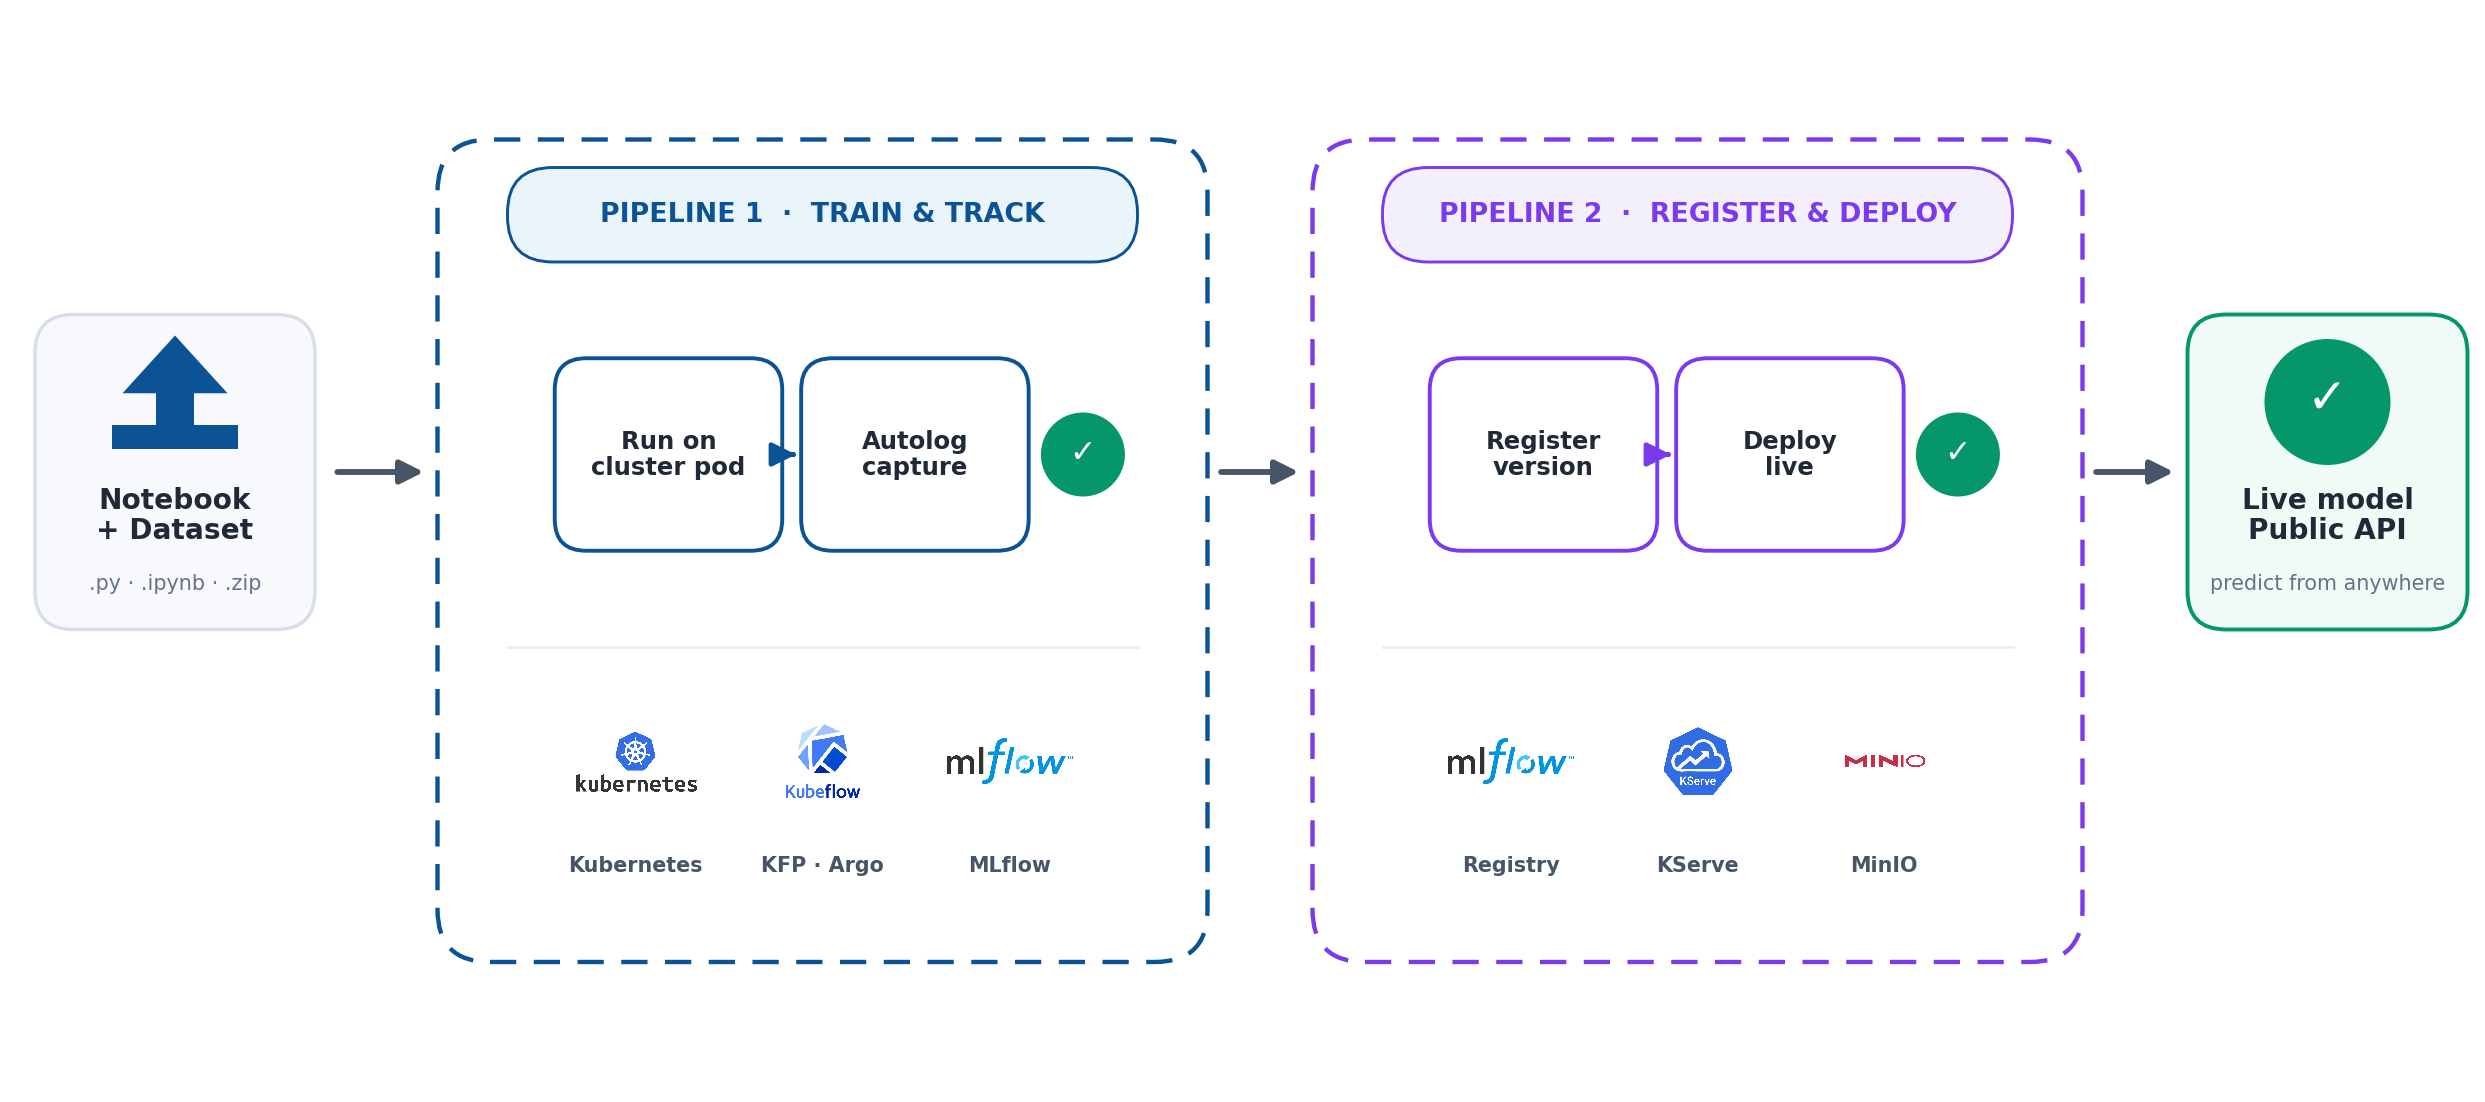
\includegraphics[width=\textwidth,keepaspectratio]{solution_pipeline}
  \caption{Proposed solution: from upload to a live model with a public API}
  \label{fig:solution-pipeline}
\end{figure}

The platform runs on a real Kubernetes cluster and ships every change to a
public URL through an automated \gls{cicd} pipeline. It is assembled entirely
from open-source components; the study of existing platforms that motivates
this choice is the subject of Chapter~\ref{chap:study}.

% ---------------------------------------------------------------------------
\section{Methodology and Planning}
\label{sec:scrum}

\subsection{Scrum Methodology}
The platform is built incrementally from independent but connected
capabilities, so an \textbf{Agile} approach was preferred over a sequential
process, and \textbf{Scrum}~\cite{scrum_guide} was adopted. Scrum organizes
work into fixed-length \emph{sprints}, each producing a potentially shippable
increment, around three artifacts (product backlog, sprint backlog, increment)
and a set of events (planning, sprint, review, retrospective).
Figure~\ref{fig:scrum} illustrates the process.

\begin{figure}[H]
  \centering
  
\includegraphics[width=0.9\textwidth,keepaspectratio]{scrum}
  \caption{The Scrum process: from product backlog to shippable increment}
  \label{fig:scrum}
\end{figure}

The Scrum roles were held as follows:
\begin{itemize}[leftmargin=1.4em]
  \item \textbf{\gls{po}}: Mr.\ Amine Gonji (company supervisor, INSOMEA),
        prioritizing the backlog and validating each increment;
  \item \textbf{\gls{sm}}: Mr.\ Ben Mardes Achref (academic supervisor),
        facilitating the process and removing impediments;
  \item \textbf{Development Team}: the author, responsible for analysis,
        design, implementation, and testing, with technical guidance from
        Mr.\ Benarous Abderrahmen.
\end{itemize}

\subsection{Sprint Organization}
The work was delivered over \textbf{four sprints in six months}, each ending
with a demonstrable, deployed increment reviewed with the supervisors
(Figure~\ref{fig:methodology-timeline}).

\begin{figure}[H]\centering
  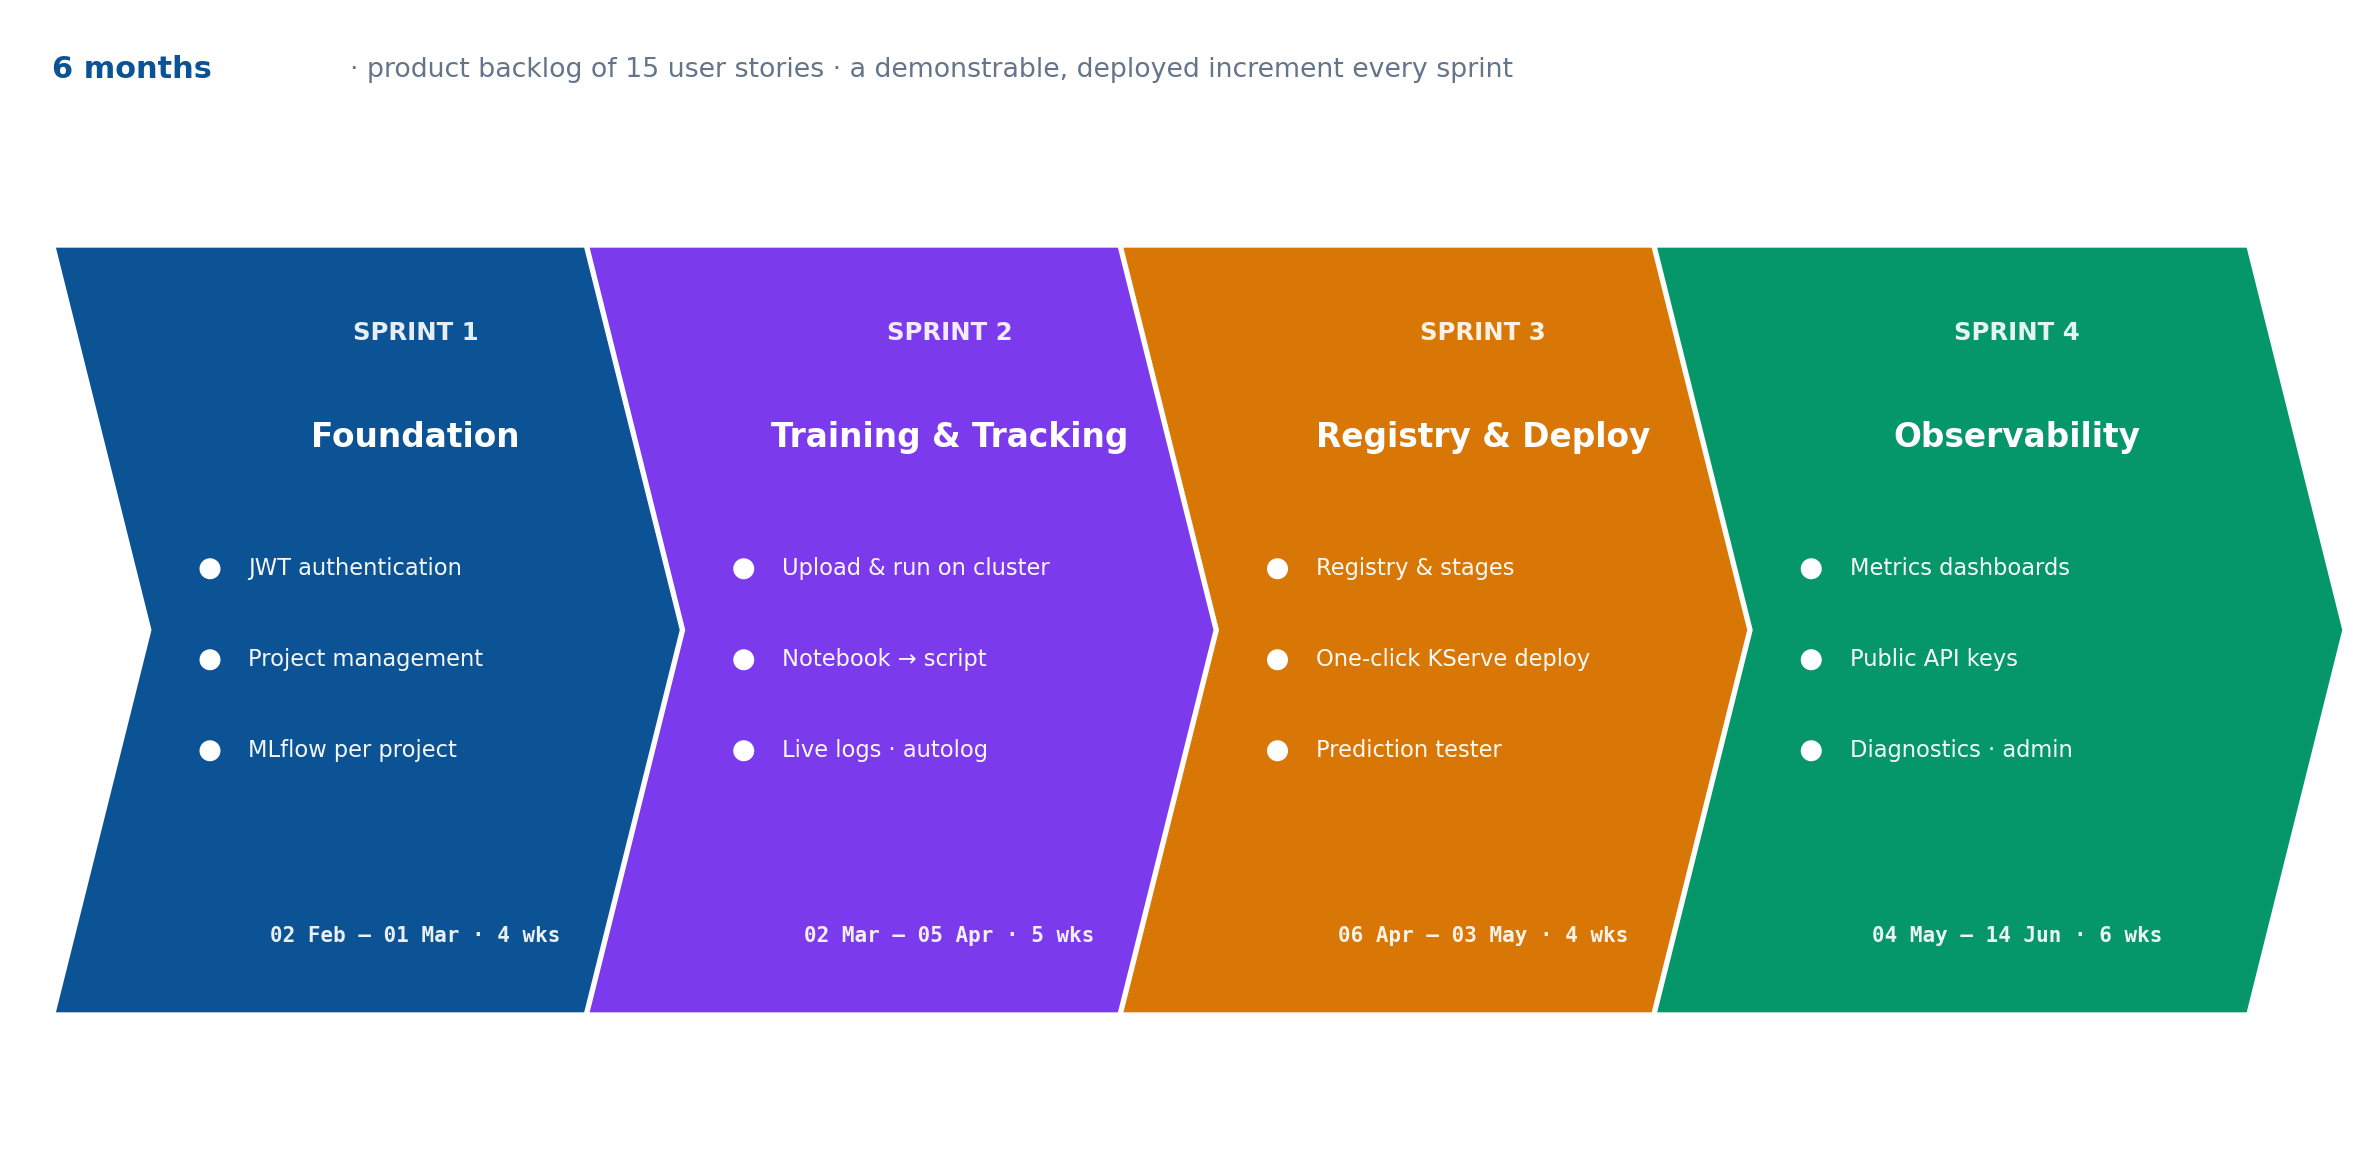
\includegraphics[width=\textwidth,keepaspectratio]{sprints}
  \caption{The four sprints and their themes}
  \label{fig:methodology-timeline}
\end{figure}

\subsection{Product Backlog}
\label{sec:backlog}
The product backlog (Table~\ref{tab:backlog}) gathers all desired capabilities
as user stories, ordered by priority; story points estimate the relative
effort.

\begin{table}[H]\centering
\caption{Product backlog}\label{tab:backlog}
\renewcommand{\arraystretch}{1.15}
\small
\begin{tabularx}{\textwidth}{|c|X|c|c|}
\hline
\rowcolor{primary!15}
\textbf{\#} & \textbf{User story} & \textbf{Prio.} & \textbf{Pts}\\
\hline
1  & As a user, I want to sign up and sign in so that my work is private.        & High & 5\\ \hline
2  & As a user, I want to create and manage projects to organize my work.        & High & 5\\ \hline
3  & As a user, I want to upload code and a dataset through the browser.         & High & 5\\ \hline
4  & As a user, I want to trigger a training run on the cluster.                 & High & 8\\ \hline
5  & As a user, I want metrics and artifacts captured automatically.             & High & 5\\ \hline
6  & As a user, I want to watch the live logs of a running pipeline.             & Med  & 3\\ \hline
7  & As a user, I want to browse and compare my experiment runs.                 & Med  & 3\\ \hline
8  & As a user, I want to register and version trained models.                   & High & 5\\ \hline
9  & As a user, I want to promote a model between Staging/Production/Archived.   & High & 3\\ \hline
10 & As a user, I want to deploy a registered model as a live service.           & High & 8\\ \hline
11 & As a user, I want to send inputs and get predictions from the UI.           & High & 5\\ \hline
12 & As a user, I want a dashboard of cluster and per-pod metrics.               & Med  & 5\\ \hline
13 & As a user, I want public API keys so external apps can call my model.       & Med  & 5\\ \hline
14 & As a user, I want clear diagnostics when an uploaded script fails.          & Med  & 5\\ \hline
15 & As an administrator, I want to manage users and oversee the platform.       & Med  & 5\\ \hline
\end{tabularx}
\end{table}

The split into sprints is deliberate: each sprint delivers a complete vertical
slice that the previous one makes possible. Sprint~1 establishes identity and
ownership; Sprint~2 produces tracked training runs; Sprint~3 turns them into
registered, deployed models; Sprint~4 makes the whole lifecycle observable,
externally consumable, and administrable.

\subsection{Project Schedule}
The project ran over six months, from 12 January 2026, opening with a framing
and state-of-the-art phase, followed by the four sprints, with the report
written in parallel (Table~\ref{tab:schedule}).

\begin{table}[H]\centering
\renewcommand{\arraystretch}{1.2}
\caption{Project schedule}\label{tab:schedule}
\small
\begin{tabularx}{\textwidth}{|>{\bfseries}l|c|c|X|}
\hline
\rowcolor{primary!15}
\textbf{Phase} & \textbf{Period} & \textbf{Duration} & \textbf{Main objective}\\
\hline
Framing \& SOTA & 12 Jan -- 01 Feb & 3 weeks & Framing, state of the art, environment setup\\ \hline
Sprint 1 & 02 Feb -- 01 Mar & 4 weeks & Authentication and project management\\ \hline
Sprint 2 & 02 Mar -- 05 Apr & 5 weeks & Training pipeline and experiment tracking\\ \hline
Sprint 3 & 06 Apr -- 03 May & 4 weeks & Model registry, deployment, and prediction\\ \hline
Sprint 4 & 04 May -- 14 Jun & 6 weeks & Observability, public API, and administration\\ \hline
Report writing & 12 Jan -- 11 Jul & Continuous & Drafting and revising in parallel\\ \hline
\end{tabularx}
\end{table}

\subsection{Management and Communication Tools}
The project was managed with lightweight, traceable tools:
\begin{itemize}[leftmargin=1.4em]
  \item \textbf{Git and GitHub} for version control; every increment is a
        series of commits on the main branch, continuously deployed;
  \item \textbf{Visual Studio Code} as the development environment;
  \item \textbf{a work journal and weekly reports} (journal de bord, bilans)
        documenting progress, decisions, and blockers throughout the six
        months;
  \item \textbf{regular reviews} with the company and academic supervisors at
        the end of each sprint.
\end{itemize}

% ---------------------------------------------------------------------------
\section{Conclusion}
This chapter presented the host organization, framed the problem, one
question: from a notebook to a live prediction service with no infrastructure
code, introduced the proposed platform, and set the Scrum methodology, the
backlog, and the schedule that structure the rest of this report. The next
chapter analyzes the business objectives and studies the technical landscape.

%==============================================================================
%  CHAPTER 2 — BUSINESS UNDERSTANDING AND TECHNICAL STUDY
%==============================================================================
\chapter{Business Understanding and Technical Study}
\label{chap:study}

\section{Introduction}
Before designing the platform, this chapter clarifies \emph{what} it must
achieve and \emph{on what} it should be built. It states the business
objectives and the system objectives that answer them, analyzes the existing
manual workflow against the \gls{mlops} maturity scale, studies the platforms
that already address this space, and closes with the benchmark of technologies
selected to build the solution.

% ---------------------------------------------------------------------------
\section{Business Objectives}
\label{sec:bo}
Six business objectives were fixed with the host company:
\begin{enumerate}[leftmargin=1.6em]
  \item \textbf{Train without owning infrastructure}: a data scientist should
        use cluster compute without any cloud or Kubernetes knowledge;
  \item \textbf{Never lose an experiment}: every run must be recorded and
        comparable;
  \item \textbf{Choose the best model objectively}: model selection must rest
        on evaluation metrics, not memory or habit;
  \item \textbf{Ship a model like software}: versioned, promoted, deployed in
        a repeatable way;
  \item \textbf{Let external applications consume models}: a deployed model
        must be usable by any website or service;
  \item \textbf{Operate and trust the system}: usage, health, and failures
        must be visible and explainable.
\end{enumerate}

% ---------------------------------------------------------------------------
\section{System Objectives}
\label{sec:so}
Each business objective maps to a delivered system capability, summarized in
Figure~\ref{fig:bodso}.

\begin{figure}[H]\centering
  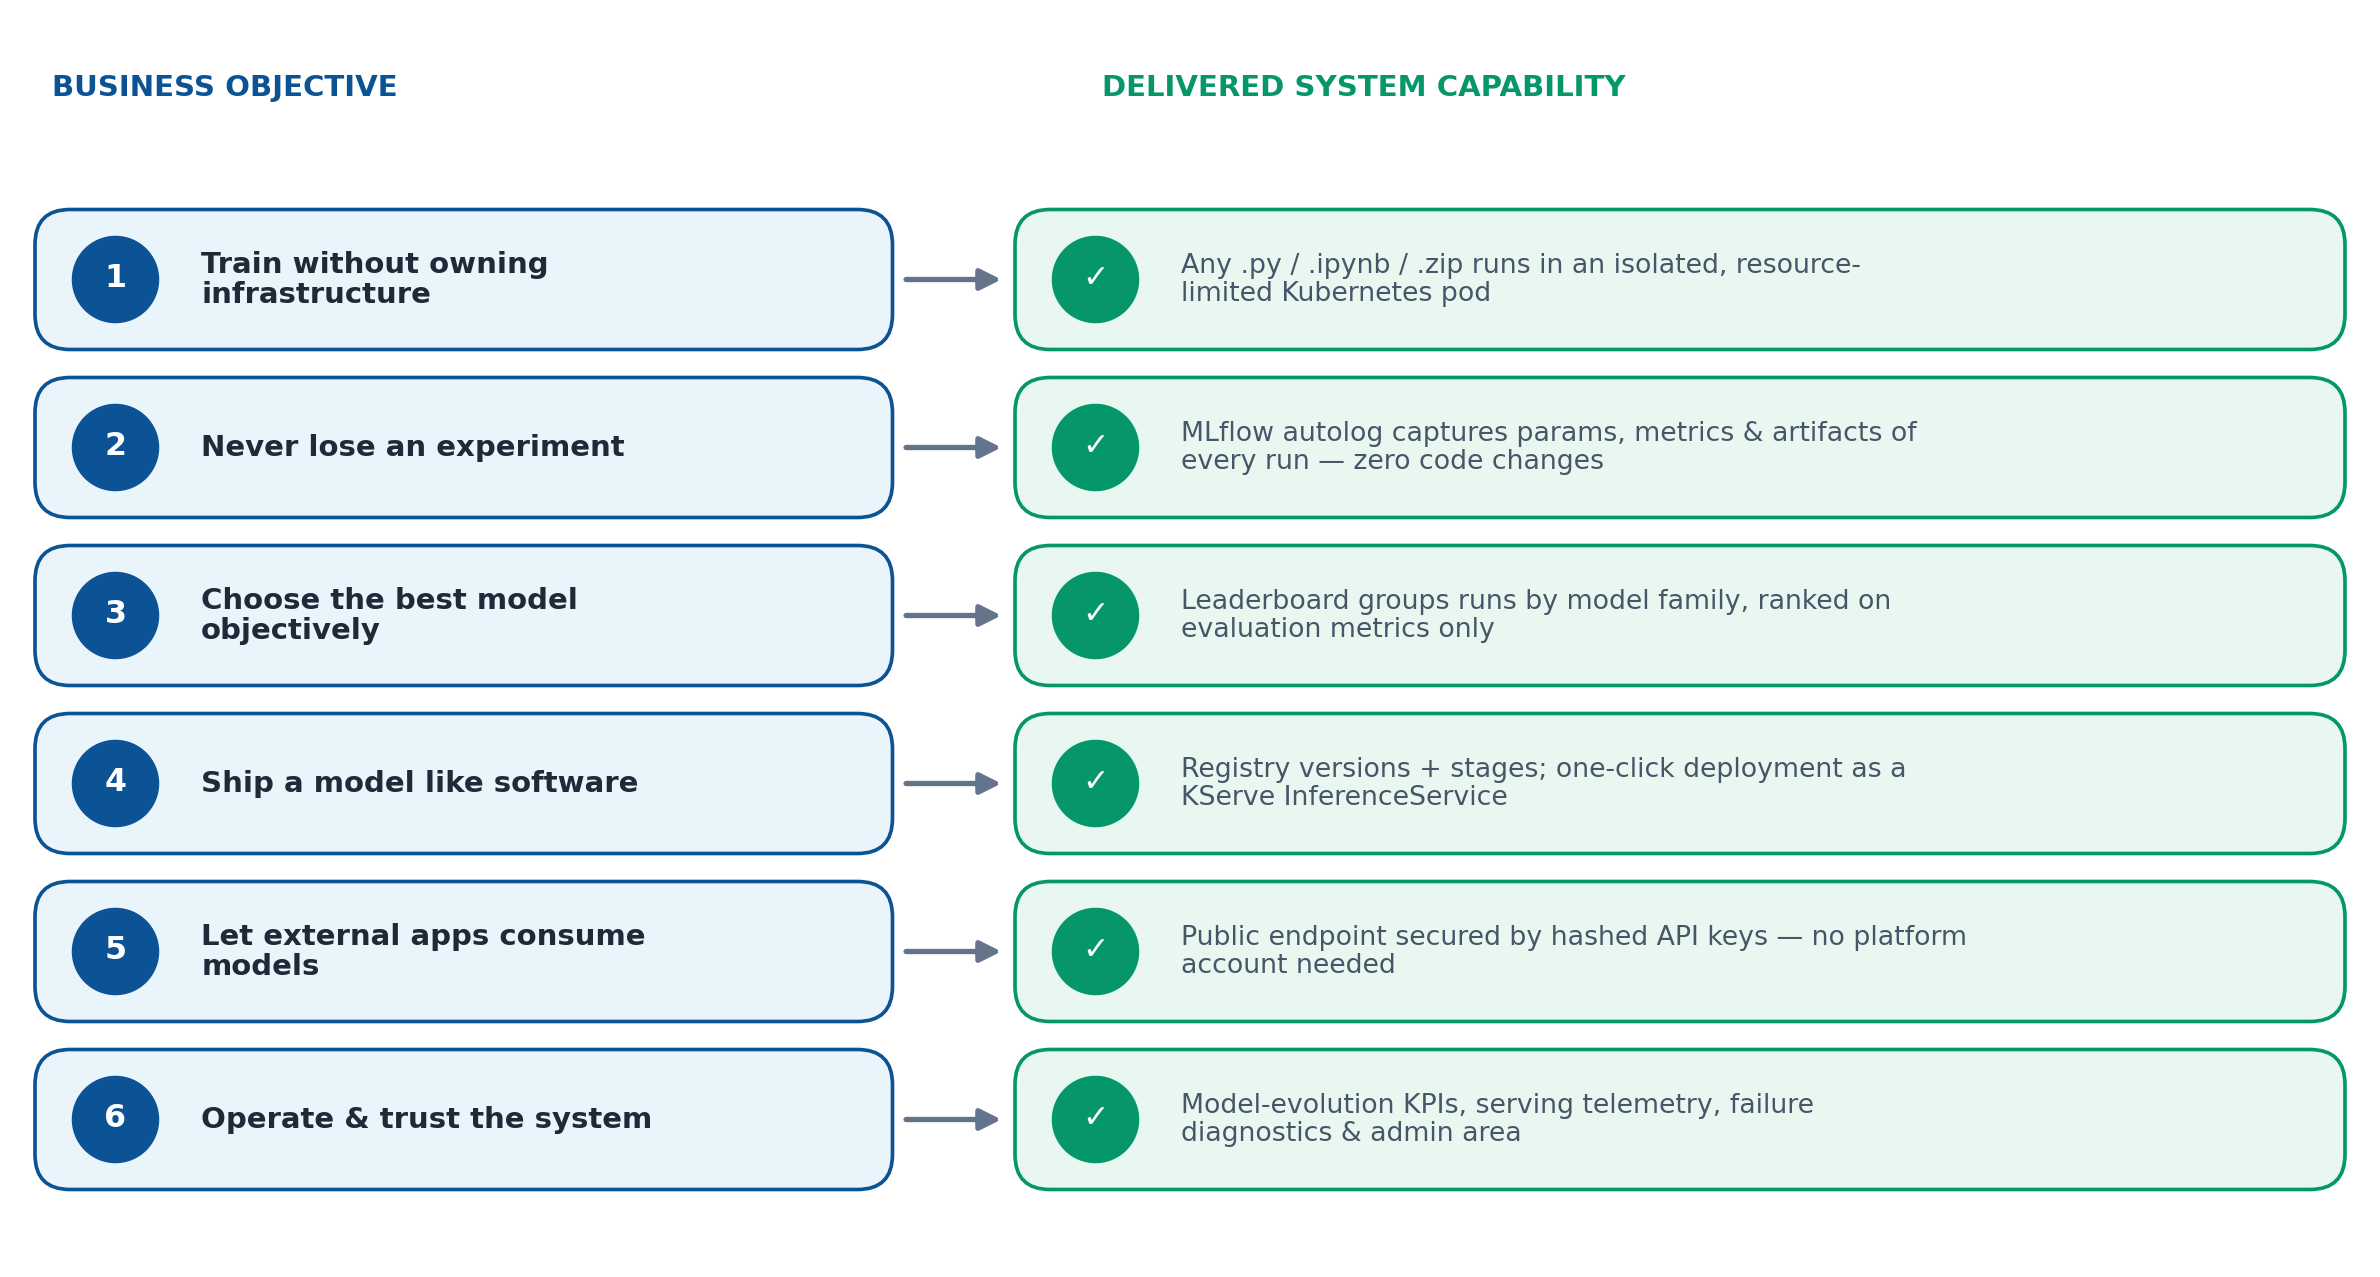
\includegraphics[width=\textwidth,keepaspectratio]{bodso}
  \caption{From business objectives to delivered system capabilities}
  \label{fig:bodso}
\end{figure}

Concretely: any \texttt{.py} / \texttt{.ipynb} / \texttt{.zip} runs in an
isolated, resource-limited Kubernetes pod (1); MLflow autolog captures
parameters, metrics, and artifacts of every run with zero code changes (2); a
leaderboard groups runs by model family and ranks them on evaluation metrics
only (3); the registry versions and stages models, and one click deploys a
version as a KServe \texttt{InferenceService} (4); a public endpoint secured
by hashed \gls{api} keys serves external applications without a platform
account (5); and serving telemetry, model-evolution \glspl{kpi}, failure
diagnostics, and an administration area make the system operable (6).

% ---------------------------------------------------------------------------
\section{Analysis of the Existing Workflow}
\label{sec:existing}
Google's reference architecture for \gls{mlops}~\cite{google_mlops} classifies
organizations into three maturity levels, a useful yardstick for evaluating
both the current situation and the target:
\begin{itemize}[leftmargin=1.4em]
  \item \textbf{Level 0, manual process}: every step is manual and
        script-driven, with a complete disconnection between the data
        scientists who produce models and the engineers who serve them. The
        notebook-on-a-laptop workflow of Chapter~\ref{chap:context} sits
        squarely at this level.
  \item \textbf{Level 1, ML pipeline automation}: training is automated as a
        re-executable pipeline; experiments are tracked; models are versioned
        in a registry and deployed through a repeatable process.
  \item \textbf{Level 2, CI/CD pipeline automation}: the pipeline itself is
        built, tested, and deployed automatically; retraining can be triggered
        by new data or detected drift.
\end{itemize}
The platform built in this project takes a team from level~0 to level~1, and
part of the way to level~2: the application itself is continuously built and
deployed through \gls{cicd}, while retraining remains user-triggered
(Figure~\ref{fig:maturity-ladder}).

\begin{figure}[H]\centering
\begin{tikzpicture}[
  lvl/.style={rounded corners=6pt, align=center, text width=3.5cm,
    minimum height=2.4cm, inner sep=6pt, font=\small, softshadow}]
  % three maturity levels, left to right, same height
  \node[lvl, draw=diagslate!40, fill=diagslate!6, text=diagslate] (l0) at (0,0)
    {{\scriptsize\bfseries LEVEL 0}\\[3pt]{\bfseries Manual process}\\[4pt]
     {\footnotesize Notebooks, scripts,\\ hand-made deploys}};
  \node[lvl, draw=diaggreen!65, line width=1.2pt, fill=diaggreen!12, text=diagslate] (l1) at (5,0)
    {{\scriptsize\bfseries\textcolor{diaggreen!45!black}{LEVEL 1}}\\[3pt]{\bfseries ML pipeline automation}\\[4pt]
     {\footnotesize Tracked runs, registry,\\ repeatable deploys}};
  \node[lvl, draw=diagblue!40, dashed, fill=diagblue!4, text=diagslate] (l2) at (10,0)
    {{\scriptsize\bfseries\textcolor{diagblue}{LEVEL 2}}\\[3pt]{\bfseries CI/CD\\ automation}\\[4pt]
     {\footnotesize Automated retraining\\ on new data}};
  \draw[-{Latex[length=2.6mm]}, line width=1pt, draw=diagslate!55] (l0.east) -- (l1.west);
  \draw[-{Latex[length=2.6mm]}, line width=1pt, draw=diagslate!55] (l1.east) -- (l2.west);
  % what the platform delivers, annotated below, no rotated text
  \draw[-{Latex[length=3mm]}, line width=2pt, draw=diaggreen!70] (0,-1.85) -- (5,-1.85);
  \node[font=\scriptsize\bfseries, text=diaggreen!45!black, anchor=north] at (2.5,-2.05)
    {This platform: Level 0 $\rightarrow$ Level 1};
  \draw[-{Latex[length=3mm]}, line width=1.4pt, draw=diagblue!55, dashed] (5,-1.85) -- (10,-1.85);
  \node[font=\scriptsize, text=diagslate, anchor=north] at (7.5,-2.05)
    {partially (application via CI/CD)};
\end{tikzpicture}
\caption{MLOps maturity ladder and the step delivered by the platform}
\label{fig:maturity-ladder}
\end{figure}

% ---------------------------------------------------------------------------
\section{State of the Art}
\label{sec:platforms}
Several commercial and open-source systems already address this space, from
fully managed cloud services (Amazon SageMaker~\cite{sagemaker}, Google Vertex
AI~\cite{vertexai}, Azure Machine Learning~\cite{azure_ml}, Databricks) to a
commercial training platform (AIchor~\cite{aichor}) and an open-source toolkit
(Kubeflow).

The managed clouds look complete but demand a cloud expert and significant
setup (accounts, permissions, storage, SDKs) before training a single model;
they are also closed and locked to one provider. The closest system to this
project's positioning is \textbf{AIchor}, developed by InstaDeep (a company
founded in Tunisia): it distributes training workloads on a cluster through a
GitOps workflow, but its lifecycle \emph{stops at training}, it is a
proprietary product, and it still requires ``a data scientist with Docker
skills''.

The platform built here removes these barriers: it covers the \emph{full}
lifecycle through serving and public consumption by \gls{api} key, is
assembled entirely from open-source components, and needs nothing more than a
browser. Table~\ref{tab:capability-matrix} compares the platforms feature by
feature.

\begin{table}[H]\centering
\caption{Feature-by-feature capability comparison}
\label{tab:capability-matrix}
\renewcommand{\arraystretch}{1.45}
\footnotesize
\begin{tabularx}{\textwidth}{|>{\raggedright\arraybackslash}p{3.15cm}|*{4}{>{\centering\arraybackslash}X|}>{\columncolor{primary!12}\centering\arraybackslash}X|}
\hline
\rowcolor{primary!15}
\textbf{Capability} & \textbf{SageMaker $\cdot$ Vertex $\cdot$ Azure~ML} & \textbf{Data\-bricks} & \textbf{AIchor} & \textbf{Kube\-flow} & \textcolor{primary}{\textbf{This plat\-form}}\\
\hline
Full ML lifecycle (train $\to$ deploy $\to$ consume) & \capyes & \cappart & \capno & \cappart & \capyes\\ \hline
Automatic experiment tracking & \capyes & \capyes & \cappart & \cappart & \capyes\\ \hline
Model registry \& versioning & \capyes & \capyes & \capno & \cappart & \capyes\\ \hline
One-click deployment (serving) & \capyes & \cappart & \capno & \cappart & \capyes\\ \hline
Public \gls{api} for external apps & \cappart & \cappart & \capno & \capno & \capyes\\ \hline
100\% open-source $\cdot$ no lock-in & \capno & \capno & \capno & \capyes & \capyes\\ \hline
Browser-only $\cdot$ no Git/Docker & \capno & \cappart & \capno & \capno & \capyes\\ \hline
\end{tabularx}

\vspace{0.35em}
{\small \capyes~Full support \quad \cappart~Partial \quad \capno~Not available
\hfill \textbf{\textcolor{primary}{Only this platform covers every capability.}}}
\end{table}

% ---------------------------------------------------------------------------
\section{Technology Benchmark and Selection}
\label{sec:tech-study}
For each concern of the platform, an open-source technology was selected; each
choice, its justification, and its logo follow.

% one centered logo with a numbered "Figure x.y: Name" caption below it
\newcommand{\techpic}[2]{\par\vspace{2pt}{\centering #1\par\vspace{1pt}%
  \captionof{figure}{#2}\par}\vspace{6pt}}
% two logos side by side, each with its own numbered caption
\newcommand{\techpair}[4]{\par\vspace{2pt}\noindent
  \begin{minipage}[t]{0.48\linewidth}\centering #1\par\vspace{1pt}\captionof{figure}{#2}\end{minipage}\hfill
  \begin{minipage}[t]{0.48\linewidth}\centering #3\par\vspace{1pt}\captionof{figure}{#4}\end{minipage}\par\vspace{6pt}}

\paragraph{Containerization and orchestration: Docker and Kubernetes.}
Containers~\cite{docker_docs} package an application with its exact
dependencies, and \gls{k8s}~\cite{kubernetes_docs} orchestrates them at scale.
Kubernetes is not only the deployment target but a core \emph{feature} of the
product: every training job and every deployed model runs in its own
resource-limited pod, which gives the platform isolation and elasticity. The
platform runs on \gls{aks} in production and on KinD locally, with no code
changes.
\techpic{
\includegraphics[height=18mm,keepaspectratio]{kubernetes}}{Kubernetes}

\paragraph{Pipeline orchestration: Kubeflow Pipelines and Argo Workflows.}
\gls{kfp}~\cite{kubeflow_pipelines} expresses a training workflow as a small
Python graph compiled into Argo Workflows~\cite{argo_workflows}, which runs
each step as an isolated pod with scheduling, retries, and log capture handled
by Argo. The backend submits one pipeline per run and follows its progress
through the \gls{kfp} \gls{api}, which is also how live logs reach the
browser. Apache Airflow was considered but targets scheduled data workflows
rather than on-demand, per-user \gls{ml} jobs on Kubernetes.
\techpair{
\includegraphics[height=17mm,keepaspectratio]{kubeflow}}{Kubeflow Pipelines}%
  {
\includegraphics[height=17mm,keepaspectratio]{argo}}{Argo Workflows}

\paragraph{Experiment tracking and registry: MLflow.}
\textbf{MLflow}~\cite{mlflow_docs} records parameters, metrics, and artifacts
of a run through a single \texttt{mlflow.autolog()} call, and provides a
built-in \textbf{Model Registry} with Staging / Production / Archived stages.
The platform provisions one MLflow experiment per project and mirrors registry
state in its own database so the interface stays responsive.
\techpic{
\includegraphics[height=17mm,keepaspectratio]{mlflow}}{MLflow}

\paragraph{Model serving: KServe.}
\textbf{KServe}~\cite{kserve_docs} turns a declarative
\texttt{InferenceService} resource into a running Deployment, Service, and
Ingress backed by a framework-specific model server, used here in
\textbf{RawDeployment} mode. Deploying a model thus reduces to creating a
single Kubernetes resource pointing at the model artifact in object storage.
Seldon Core offers similar capabilities but with a heavier operational
footprint for a single-team platform.
\techpic{
\includegraphics[height=19mm,keepaspectratio]{kserve}}{KServe}

\paragraph{Object storage: MinIO.}
\textbf{MinIO}~\cite{minio_docs} is an \gls{s3}-compatible object store
deployed inside the cluster. It holds uploaded code, datasets, and all MLflow
artifacts, and is a drop-in for the \gls{s3} \gls{api} that MLflow, KServe,
and the AWS SDK expect.
\techpic{
\includegraphics[height=14mm,keepaspectratio]{minio}}{MinIO}

\paragraph{Database: PostgreSQL.}
A single \textbf{PostgreSQL}~\cite{postgresql_docs} instance stores both the
platform's own tables and MLflow's tracking tables, keeping operations simple.
The backend accesses it asynchronously through SQLAlchemy~2, so database I/O
never blocks the event loop.
\techpic{
\includegraphics[height=16mm,keepaspectratio]{postgresql}}{PostgreSQL}

\paragraph{Backend: FastAPI.}
\textbf{FastAPI}~\cite{fastapi_docs} is an asynchronous Python web framework
that derives request validation and an OpenAPI schema from type hints. Python
is the natural choice because the whole machine-learning ecosystem (MLflow,
the Kubeflow SDK, the Kubernetes client) is Python. Compared with Flask or
Django, FastAPI brings native async support and generated documentation with
no extra code.
\techpic{
\includegraphics[height=16mm,keepaspectratio]{fastapi}}{FastAPI}

\paragraph{Frontend: Angular.}
\textbf{Angular}~\cite{angular_docs} is a batteries-included \gls{spa}
framework; the project uses Angular~19 with standalone components and signals,
served by NGINX. Route guards enforce authentication and the administrator
role on the client side, mirroring the backend's checks.
\techpic{
\includegraphics[height=16mm,keepaspectratio]{angular}}{Angular}

\paragraph{Secure public exposure: Cloudflare Tunnel.}
The platform is published through a \textbf{Cloudflare
Tunnel}~\cite{cloudflare_tunnel}: an in-cluster agent opens an outbound-only
connection, so no public IP address or inbound port is exposed. Public traffic
is terminated at Cloudflare's edge over \gls{https} and passes through its
protections, including \gls{ddos} mitigation.
\techpic{
\includegraphics[height=15mm,keepaspectratio]{cloudflare}}{Cloudflare Tunnel}

\paragraph{CI/CD: GitHub Actions and Azure Container Registry.}
Every push to the main branch triggers a \textbf{GitHub Actions} workflow that
builds the backend and frontend images, pushes them to \textbf{\gls{acr}},
and upgrades the cluster deployment.
\techpair{
\includegraphics[height=17mm,keepaspectratio]{github_actions}}{GitHub Actions}%
  {
\includegraphics[height=17mm,keepaspectratio]{acr}}{Azure Container Registry}

\medskip
Table~\ref{tab:software} summarizes the final technical choices, together with
the working environment.

\begin{table}[H]\centering
\renewcommand{\arraystretch}{1.2}
\caption{Final technical choices}\label{tab:software}
\small
\begin{tabularx}{\textwidth}{|>{\raggedright\arraybackslash}p{4.2cm}|X|}
\hline
\rowcolor{primary!15}
\textbf{Concern} & \textbf{Selected technology}\\
\hline
Backend             & FastAPI (Python~3.11), SQLAlchemy~2 (async), Pydantic~v2\\
\hline
Frontend            & Angular~19 (standalone components, signals), Tailwind\\
\hline
Database            & PostgreSQL~16 (platform + MLflow)\\
\hline
Object storage      & MinIO (\gls{s3}-compatible)\\
\hline
Experiment tracking & MLflow (tracking + registry)\\
\hline
Orchestration       & Kubernetes (\gls{aks} / KinD), \gls{kfp}, Argo Workflows\\
\hline
Model serving       & KServe (RawDeployment)\\
\hline
Networking          & Cloudflare Tunnel (\gls{tls} at the edge)\\
\hline
CI/CD               & GitHub Actions, \gls{acr}\\
\hline
Development         & Visual Studio Code, Git/GitHub, Docker\\
\hline
Modeling \& report  & \gls{uml} (PlantUML, draw.io), \LaTeX\\
\hline
Hardware            & Intel Core i7 / 16\,GB workstation; \gls{aks} cluster\\
\hline
\end{tabularx}
\end{table}

% ---------------------------------------------------------------------------
\section{Conclusion}
This chapter fixed the business and system objectives, situated the existing
manual workflow at maturity level~0, showed that no existing platform covers
every needed capability, and selected an open-source technology for each
concern. The next chapter designs the system built on these choices.

%==============================================================================
%  CHAPTER 3 — SYSTEM DESIGN
%==============================================================================
\chapter{System Design}
\label{chap:requirements}
\label{chap:design}

\section{Introduction}
This chapter designs the system as a whole, before the next chapter details
its realization sprint by sprint. It presents the functional view (actors,
requirements, and use cases), the global architecture in its logical and
physical forms, the organization of the two pipelines, the detailed dynamic
design through sequence diagrams, and the data model.

% ---------------------------------------------------------------------------
\section{Functional View}
\label{sec:functional-view}

\subsection{Actors}
Four actors interact with the system:
\begin{itemize}[leftmargin=1.4em]
  \item \textbf{Platform user (data scientist)} --- the primary actor: manages
        projects, uploads code and data, triggers and follows training runs,
        compares experiments, registers, promotes, deploys, and tests models,
        and manages the \gls{api} keys that expose a deployment publicly. No
        infrastructure knowledge is assumed: every cluster interaction happens
        behind a button.
  \item \textbf{External API client} --- a third-party website, mobile
        application, or backend that calls a deployed model's public endpoint
        with an \gls{api} key. It has no platform account; its whole contract
        is one authenticated \gls{http} call.
  \item \textbf{Administrator} --- inherits all user capabilities and, in
        addition, manages accounts and roles and oversees every user's
        projects, pipelines, and deployments.
  \item \textbf{System (automated actors)} --- the training pipeline and the
        model server act on the user's behalf once triggered; they appear as
        participants in the sequence diagrams.
\end{itemize}

\subsection{Functional Requirements}
The platform must provide the following functional capabilities, grouped by
module:
\begin{itemize}[leftmargin=1.4em]
  \item \textbf{Authentication and sessions}: sign up, sign in, refresh the
        access token, and retrieve the current user's profile and role.
  \item \textbf{Project management}: create, list, update, and delete projects;
        bind each project to its own tracking experiment; enforce strict
        per-owner isolation (foreign resources return \texttt{404}).
  \item \textbf{Upload and code handling}: upload code
        (\texttt{.py}, \texttt{.ipynb}, \texttt{.zip}) and datasets;
        auto-detect the entry script; convert notebooks to runnable scripts;
        run a pre-flight static analysis that warns about common pitfalls.
  \item \textbf{Training execution}: trigger a training run in an isolated
        cluster pod, stream its logs live to the browser, and install missing
        dependencies automatically.
  \item \textbf{Experiment tracking}: capture parameters, metrics, and
        artifacts of every run automatically; browse and compare runs; open a
        run-details view with an artifact browser (list, preview, download).
  \item \textbf{Model registry}: register a run as a versioned model, list its
        versions, and promote them across Staging / Production / Archived.
  \item \textbf{Deployment}: deploy a registered version as a live service in
        one click, detect the model framework automatically
        (scikit-learn / XGBoost), track the deployment status and endpoint, and
        delete a deployment.
  \item \textbf{Prediction}: test predictions from the interface, with readable
        error reporting when an input or the model server fails.
  \item \textbf{Public API and keys}: create, list, and revoke per-deployment
        \gls{api} keys (stored hashed); serve a public, key-authenticated
        prediction endpoint; generate ready-to-paste code snippets.
  \item \textbf{Monitoring}: display live cluster and per-pod resource metrics,
        and a per-project serving view with request volume, error rate, latency,
        and timeline, traffic split by origin (tester versus public \gls{api}),
        and a per-deployment breakdown including each model's live \gls{cpu} and
        memory usage.
  \item \textbf{Insights}: track each model's evolution across versions with
        evaluation \glspl{kpi}, a health verdict, and version/stage progression.
  \item \textbf{Diagnostics}: capture and surface the failure reason of a
        failed run so the user understands \emph{why} it failed.
  \item \textbf{Administration}: manage user accounts (activate, deactivate,
        promote, demote, purge, delete), consult platform-wide statistics, and
        oversee every user's projects, pipelines, and deployments
        (administrator only).
\end{itemize}

\subsection{Non-Functional Requirements}
\begin{itemize}[leftmargin=1.4em]
  \item \textbf{Security}: stateless \gls{jwt} authentication~\cite{rfc7519};
        passwords stored as bcrypt hashes and \gls{api} keys as \gls{sha}-256
        hashes~\cite{owasp_api}; strict ownership checks; administrator-only
        endpoints.
  \item \textbf{Performance}: a fully asynchronous backend, so slow external
        calls never block other requests.
  \item \textbf{Scalability and isolation}: every training job and model
        server runs in its own resource-limited pod.
  \item \textbf{Portability}: identical behavior on a local KinD cluster and
        on \gls{aks}, everything expressed as Kubernetes resources.
  \item \textbf{Reproducibility}: code, parameters, metrics, and artifacts of
        every run captured automatically.
  \item \textbf{Usability}: the whole lifecycle from one web interface; no
        kubectl, no \gls{yaml}, no cloud console.
\end{itemize}

\subsection{Global Use-Case Diagram}
\label{sec:usecases}
Figure~\ref{fig:usecase-global} summarizes the interactions of the three human
actors with the system.
\begin{figure}[H]\centering
  
\includegraphics[width=0.95\textwidth,height=0.48\textheight,keepaspectratio]{usecase_global}
  \caption{Global use-case diagram of the platform}
  \label{fig:usecase-global}
\end{figure}

\subsection{Use-Case Refinements}
Tables~\ref{tab:uc-signin} to~\ref{tab:uc-public} refine one central use case
per lifecycle area; the remaining flows are detailed by the sequence diagrams
of Section~\ref{sec:seq-diagrams}.

\begin{table}[H]\centering
\renewcommand{\arraystretch}{1.2}
\caption{Textual description of the ``Sign in'' use case}\label{tab:uc-signin}
\begin{tabularx}{\textwidth}{|>{\bfseries}p{3.2cm}|X|}
\hline
Use case & Sign in\\ \hline
Actor & Platform user\\ \hline
Precondition & The user already has a registered account.\\ \hline
Post-condition & The user is authenticated; an access/refresh token pair is issued.\\ \hline
Nominal scenario & 1.~The user submits email and password.\newline 2.~The system verifies the password against its stored hash.\newline 3.~The system issues a \gls{jwt} access token and a refresh token.\newline 4.~The user is redirected to the dashboard.\\ \hline
Exceptions & Invalid credentials: the request is rejected with a clear error.\\ \hline
\end{tabularx}
\end{table}

\begin{table}[H]\centering
\renewcommand{\arraystretch}{1.2}
\caption{Textual description of the ``Trigger a training run'' use case}\label{tab:uc-train}
\begin{tabularx}{\textwidth}{|>{\bfseries}p{3.2cm}|X|}
\hline
Use case & Trigger a training run\\ \hline
Actor & Platform user\\ \hline
Precondition & The user is authenticated and has uploaded code (and optionally a dataset) to a project.\\ \hline
Post-condition & A pipeline run executes on the cluster; its metrics, parameters, and artifacts are recorded.\\ \hline
Nominal scenario & 1.~The user clicks ``Run code''.\newline 2.~The backend submits a pipeline to the orchestrator.\newline 3.~An isolated pod downloads the code, installs dependencies, and runs the entry script.\newline 4.~The autolog wrapper records results to the tracking server.\newline 5.~The user follows the live logs and the captured metrics.\\ \hline
Exceptions & The script fails: the error is captured and surfaced to the user; no model is registered.\\ \hline
\end{tabularx}
\end{table}

\begin{table}[H]\centering
\renewcommand{\arraystretch}{1.2}
\caption{Textual description of the ``Deploy a model'' use case}\label{tab:uc-deploy}
\begin{tabularx}{\textwidth}{|>{\bfseries}p{3.2cm}|X|}
\hline
Use case & Deploy a model\\ \hline
Actor & Platform user\\ \hline
Precondition & A model version is registered in the registry.\\ \hline
Post-condition & A live prediction service is running and reachable on the cluster.\\ \hline
Nominal scenario & 1.~The user clicks ``Deploy'' on a registered model.\newline 2.~The backend detects the model's framework and creates an \texttt{InferenceService}.\newline 3.~The serving operator reconciles it into a Deployment, Service, and Ingress.\newline 4.~The model server loads the artifact from object storage.\newline 5.~The status and endpoint are reported back to the user.\\ \hline
Exceptions & The service fails to become ready: the deployment is marked failed and the user is notified.\\ \hline
\end{tabularx}
\end{table}

\begin{table}[H]\centering
\renewcommand{\arraystretch}{1.2}
\caption{Textual description of the ``Call the public prediction endpoint'' use case}\label{tab:uc-public}
\begin{tabularx}{\textwidth}{|>{\bfseries}p{3.2cm}|X|}
\hline
Use case & Call the public prediction endpoint\\ \hline
Actor & External \gls{api} client\\ \hline
Precondition & The model is deployed and the client holds a valid \gls{api} key.\\ \hline
Post-condition & The client receives a prediction from the deployed model.\\ \hline
Nominal scenario & 1.~The client sends a request with an \texttt{Authorization: Bearer} key.\newline 2.~The backend hashes the key and looks it up, scoped to the deployment.\newline 3.~The backend confirms the deployment is ready.\newline 4.~The request is forwarded to the model server.\newline 5.~The prediction is returned to the client.\\ \hline
Exceptions & Invalid or revoked key: the backend returns \texttt{401}.\\ \hline
\end{tabularx}
\end{table}

% ---------------------------------------------------------------------------
\section{Global Architecture}
\label{sec:architecture}

\subsection{Logical Architecture}
\label{sec:app-architecture}
The application adopts a \textbf{four-tier layered architecture}
(Figure~\ref{fig:layered-arch}):
\begin{itemize}[leftmargin=1.4em]
  \item \textbf{Presentation}: an Angular single-page application consuming
        the backend's \gls{rest} \gls{api};
  \item \textbf{API}: FastAPI routers that validate requests and enforce
        authentication and ownership;
  \item \textbf{Service}: the business logic orchestrating the cluster systems
        (pipelines, MLflow, KServe, object storage);
  \item \textbf{Data}: SQLAlchemy models mapped onto PostgreSQL.
\end{itemize}

\begin{figure}[H]\centering
  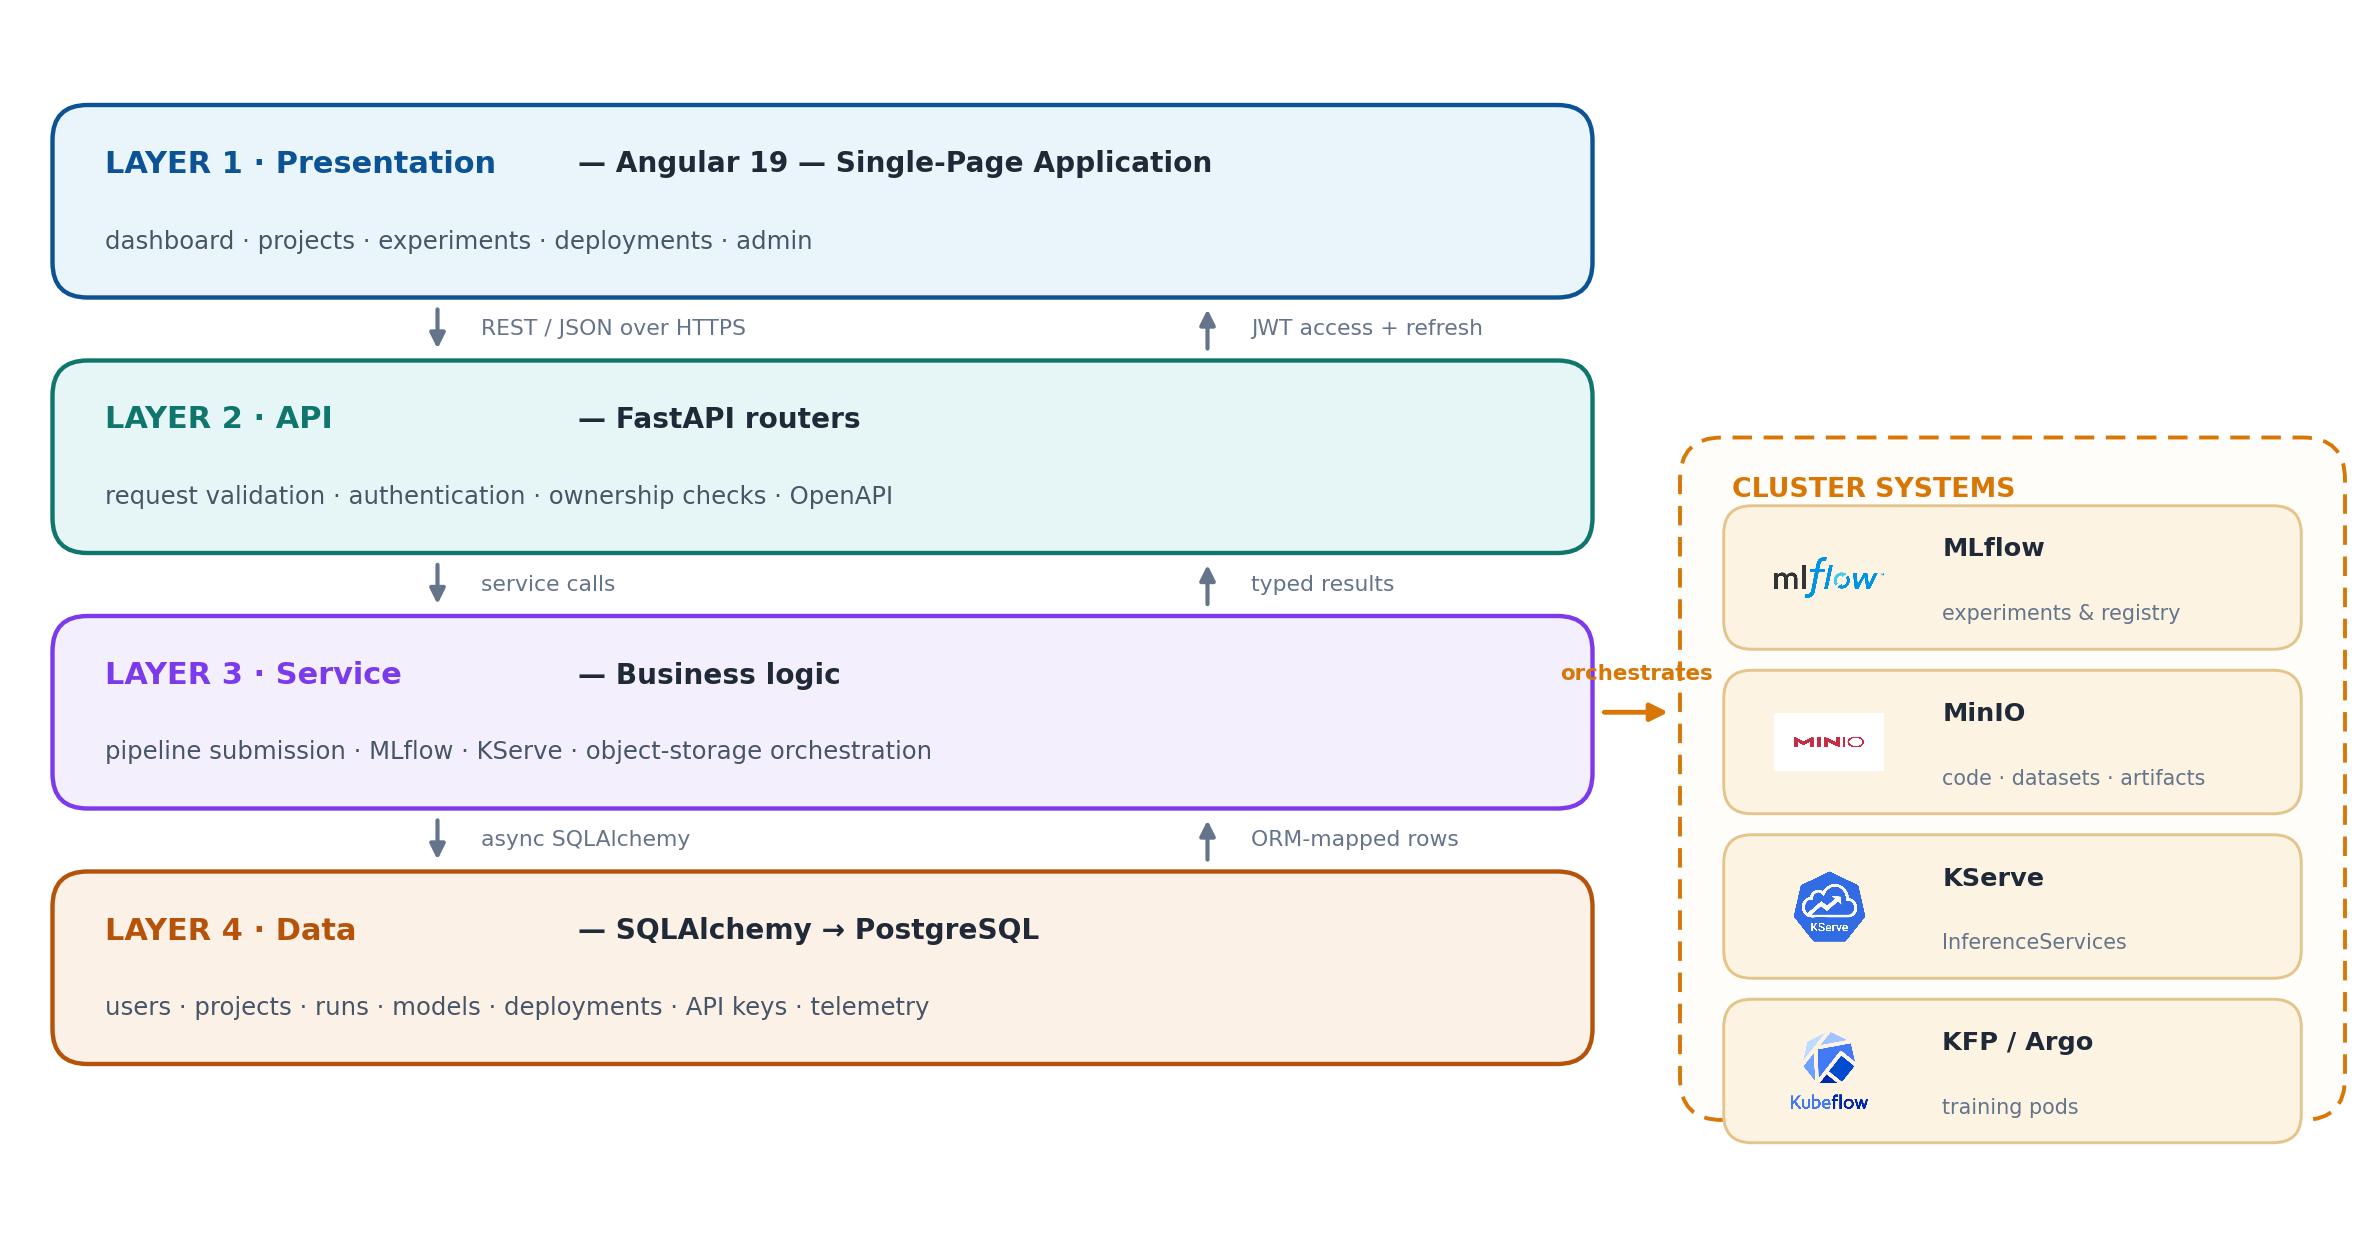
\includegraphics[width=\textwidth,keepaspectratio]{logical_arch}
  \caption{Four-tier layered architecture and the cluster systems it orchestrates}
  \label{fig:layered-arch}
\end{figure}

The layered style was preferred over microservices for proportionality: the
platform already delegates its heavyweight concerns (pipeline execution, model
serving, artifact storage) to dedicated cluster components. The result is one
backend image and one frontend image, each independently deployable.

\subsection{Physical Architecture}
\label{sec:physical}
Everything runs on one Kubernetes cluster --- \gls{aks} in production, KinD
locally, same code. Public traffic follows the path \emph{browser
$\rightarrow$ Cloudflare edge (\gls{tls}) $\rightarrow$ tunnel agent
$\rightarrow$ frontend $\rightarrow$ backend $\rightarrow$ cluster systems}.
Figure~\ref{fig:physical-arch} shows the topology: the platform's own
workloads run as long-lived deployments, while training jobs and model servers
are created and destroyed on demand, each in its own resource-limited pod.

\begin{figure}[H]\centering
  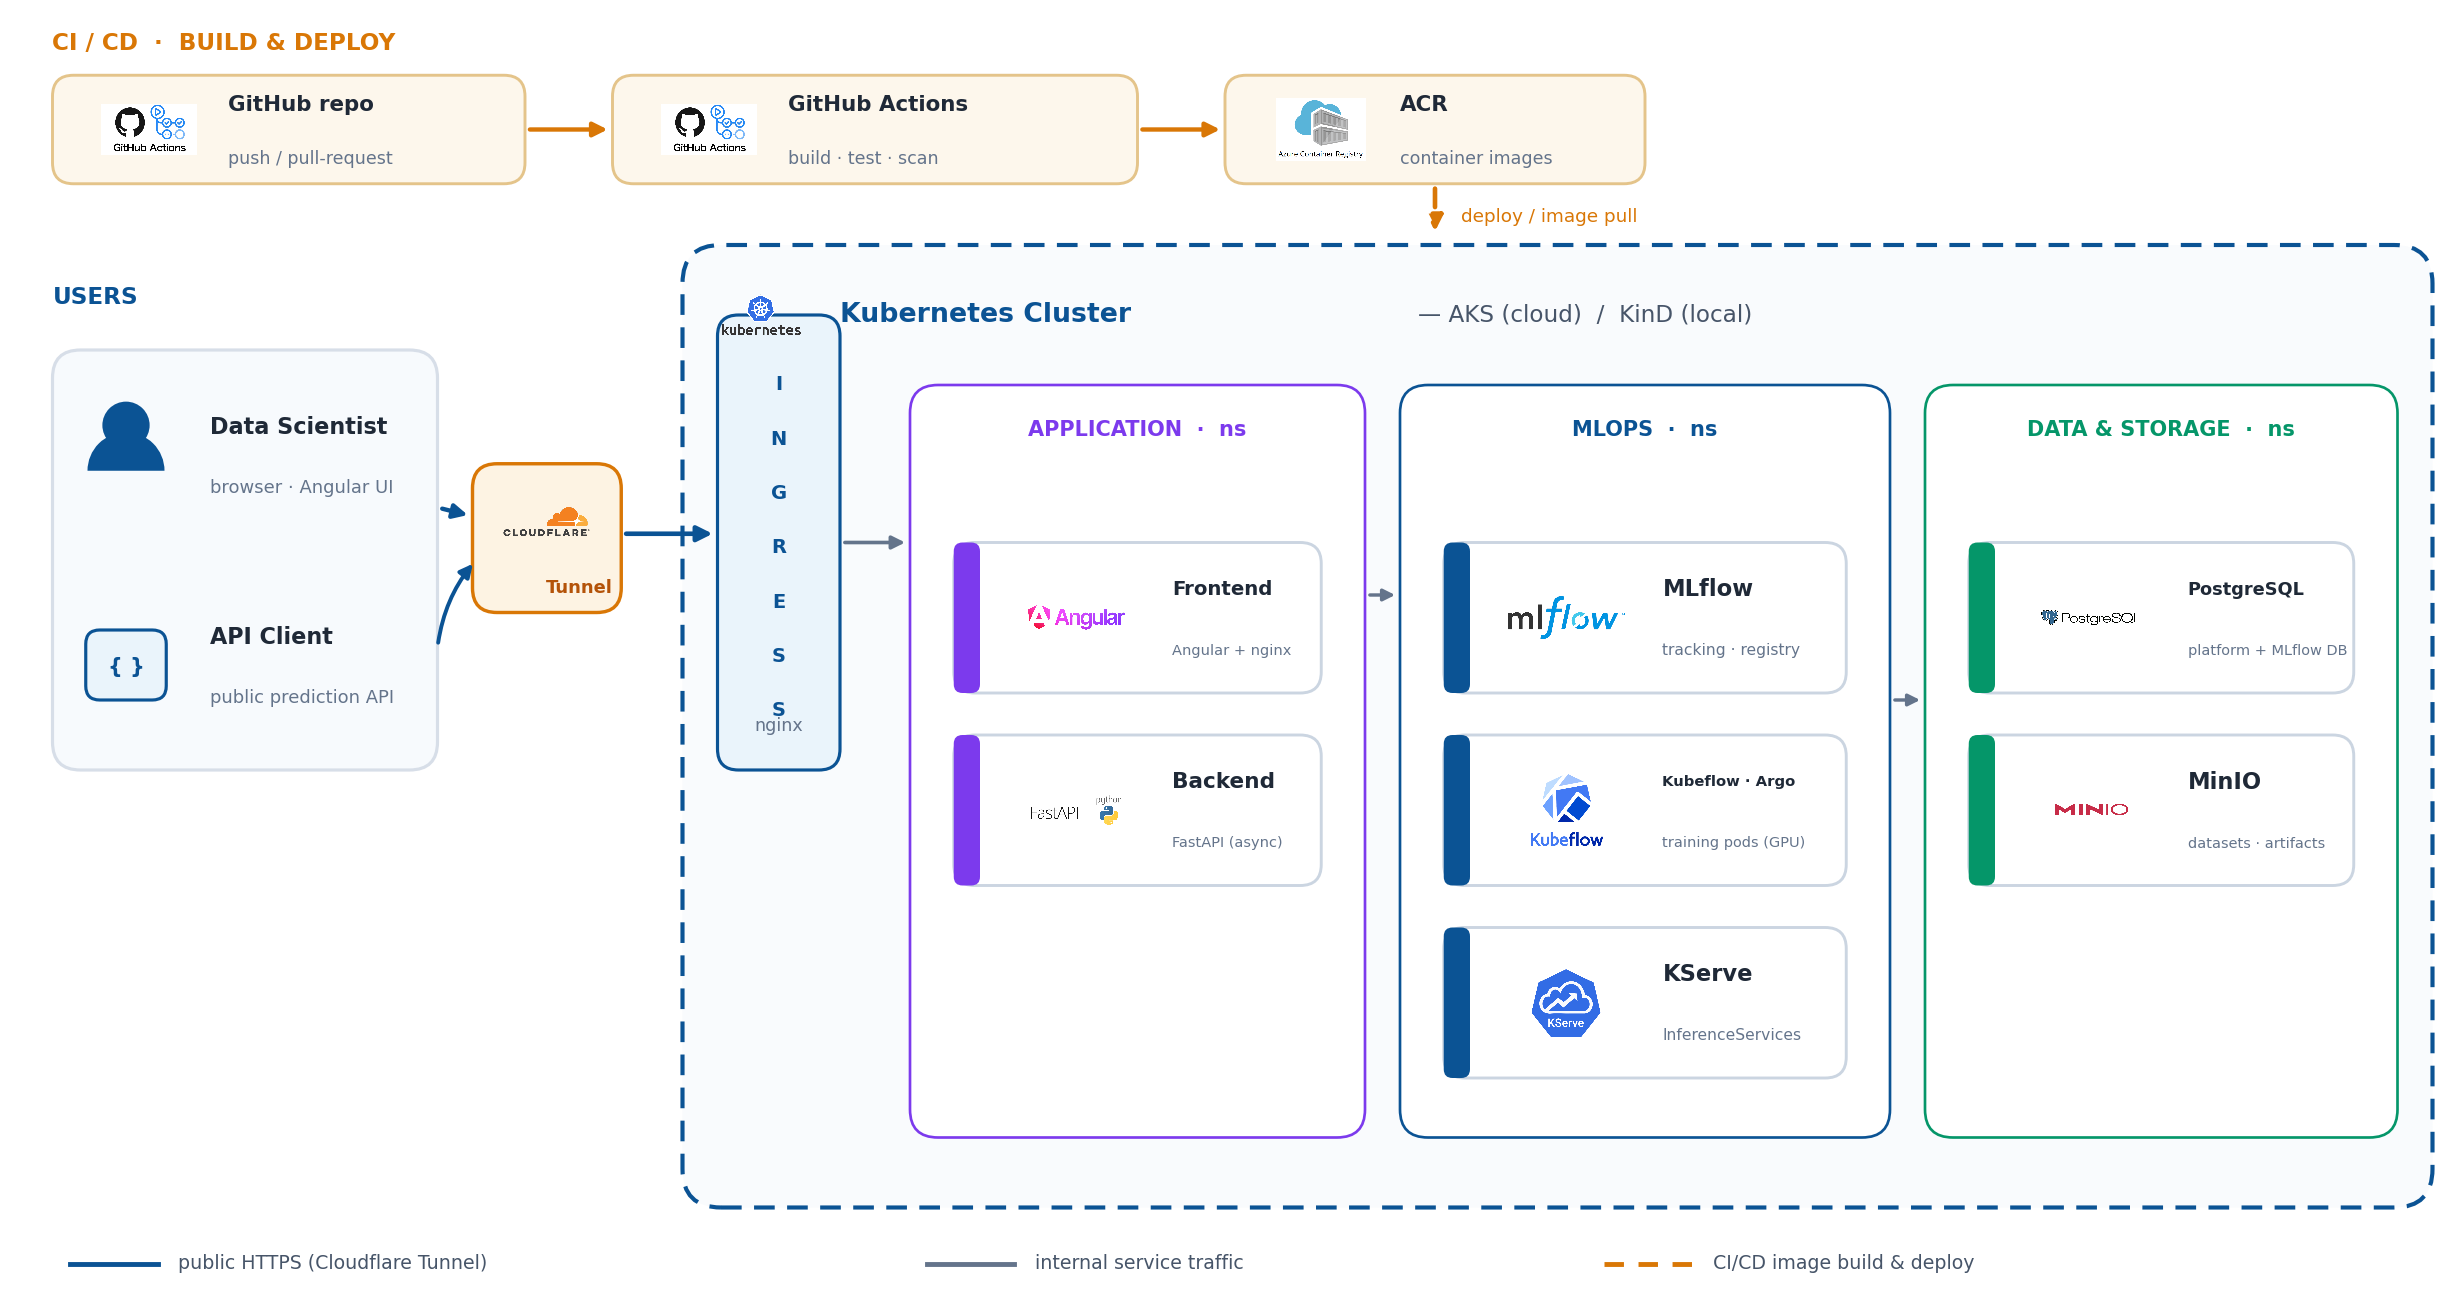
\includegraphics[width=\textwidth,height=0.55\textheight,keepaspectratio]{physical_arch}
  \caption{Physical architecture of the platform on the Kubernetes cluster}
  \label{fig:physical-arch}
\end{figure}

% ---------------------------------------------------------------------------
\section{Pipeline Organization}
\label{sec:pipeline-org}
Two flows structure the whole system: a training path and a serving path. They
meet only in the object store and the registry --- training produces artifacts
and versions, serving consumes them --- so each half can evolve, scale, and
fail independently.

The \textbf{training path} starts from an upload: the backend stores code and
dataset in the object store, then submits a \gls{kfp} pipeline whose single
step runs in an isolated pod and executes the user's code under an autolog
wrapper (Figure~\ref{fig:pipeline-flow}).

\begin{figure}[H]\centering
\resizebox{\textwidth}{!}{%
\begin{tikzpicture}
  \node[stagenode,fill=diagblue!12] (trig) {Trigger\\run};
  \node[stepnode,right=1.5cm of trig] (dl) {Download\\code + data};
  \node[stepnode,right=0.5cm of dl] (dep) {Install\\dependencies};
  \node[stepnode,right=0.5cm of dep] (conv) {Convert\\notebook};
  \node[stepnode,right=0.5cm of conv] (run) {Autolog\\runner + run};
  \node[storenode,right=1.5cm of run] (ml) {
\includegraphics[height=0.5cm]{mlflow}\\metrics \textperiodcentered{} params\\artifacts};
  \node[stagenode,below=1.1cm of conv,fill=diaggreen!10,draw=diaggreen!60] (logs) {Live logs\\$\rightarrow$ UI};
  \begin{scope}[on background layer]
    \node[clusterbox,fit=(dl)(dep)(conv)(run),
          label={[font=\scriptsize\bfseries,text=diagblue]above:{Isolated pod (Kubernetes)}}] (pod) {};
  \end{scope}
  \draw[flowarrow] (trig) -- (dl);
  \draw[flowarrow] (dl) -- (dep);
  \draw[flowarrow] (dep) -- (conv);
  \draw[flowarrow] (conv) -- (run);
  \draw[flowarrow] (run) -- (ml);
  \draw[flowarrow,draw=diaggreen!70] (pod.south) -- (logs);
\end{tikzpicture}}
\caption{Training path: from trigger to captured experiment}
\label{fig:pipeline-flow}
\end{figure}

The \textbf{serving path} starts from the registry: a registered model version
is deployed by creating one declarative \texttt{InferenceService} resource,
which the serving operator reconciles into a running model server loading its
artifact from the object store (Figure~\ref{fig:deploy-flow}).

\begin{figure}[H]\centering
\resizebox{\textwidth}{!}{%
\begin{tikzpicture}
  \node[stagenode,fill=diagblue!12] (reg) {Register\\model version};
  \node[stepnode,right=0.7cm of reg] (isvc) {Backend creates\\InferenceService};
  \node[stepnode,right=0.7cm of isvc] (op) {
\includegraphics[height=0.45cm]{kserve}\\KServe operator\\reconciles};
  \node[stepnode,right=0.7cm of op,minimum height=2.4cm] (res) {Deployment\\Service\\Ingress};
  \node[storenode,right=0.7cm of res] (srv) {Model server\\loads artifact\\
\includegraphics[height=0.4cm]{minio}};
  \node[stagenode,right=0.7cm of srv,fill=diaggreen!12,draw=diaggreen!60] (ready) {READY\\$\rightarrow$ Predict};
  \draw[flowarrow] (reg) -- (isvc);
  \draw[flowarrow] (isvc) -- (op);
  \draw[flowarrow] (op) -- (res);
  \draw[flowarrow] (res) -- (srv);
  \draw[flowarrow] (srv) -- (ready);
\end{tikzpicture}}
\caption{Serving path: from a registered model to a live prediction service}
\label{fig:deploy-flow}
\end{figure}

% ---------------------------------------------------------------------------
\section{Sequence Diagrams}
\label{sec:seq-diagrams}
The dynamic behavior of the main flows is detailed by sequence diagrams,
grouped by lifecycle area.

\subsection{Authentication}
Figures~\ref{fig:seq-signup} and~\ref{fig:seq-login} detail the sign-up and
login flows on which every later interaction depends.
\begin{figure}[H]\centering
  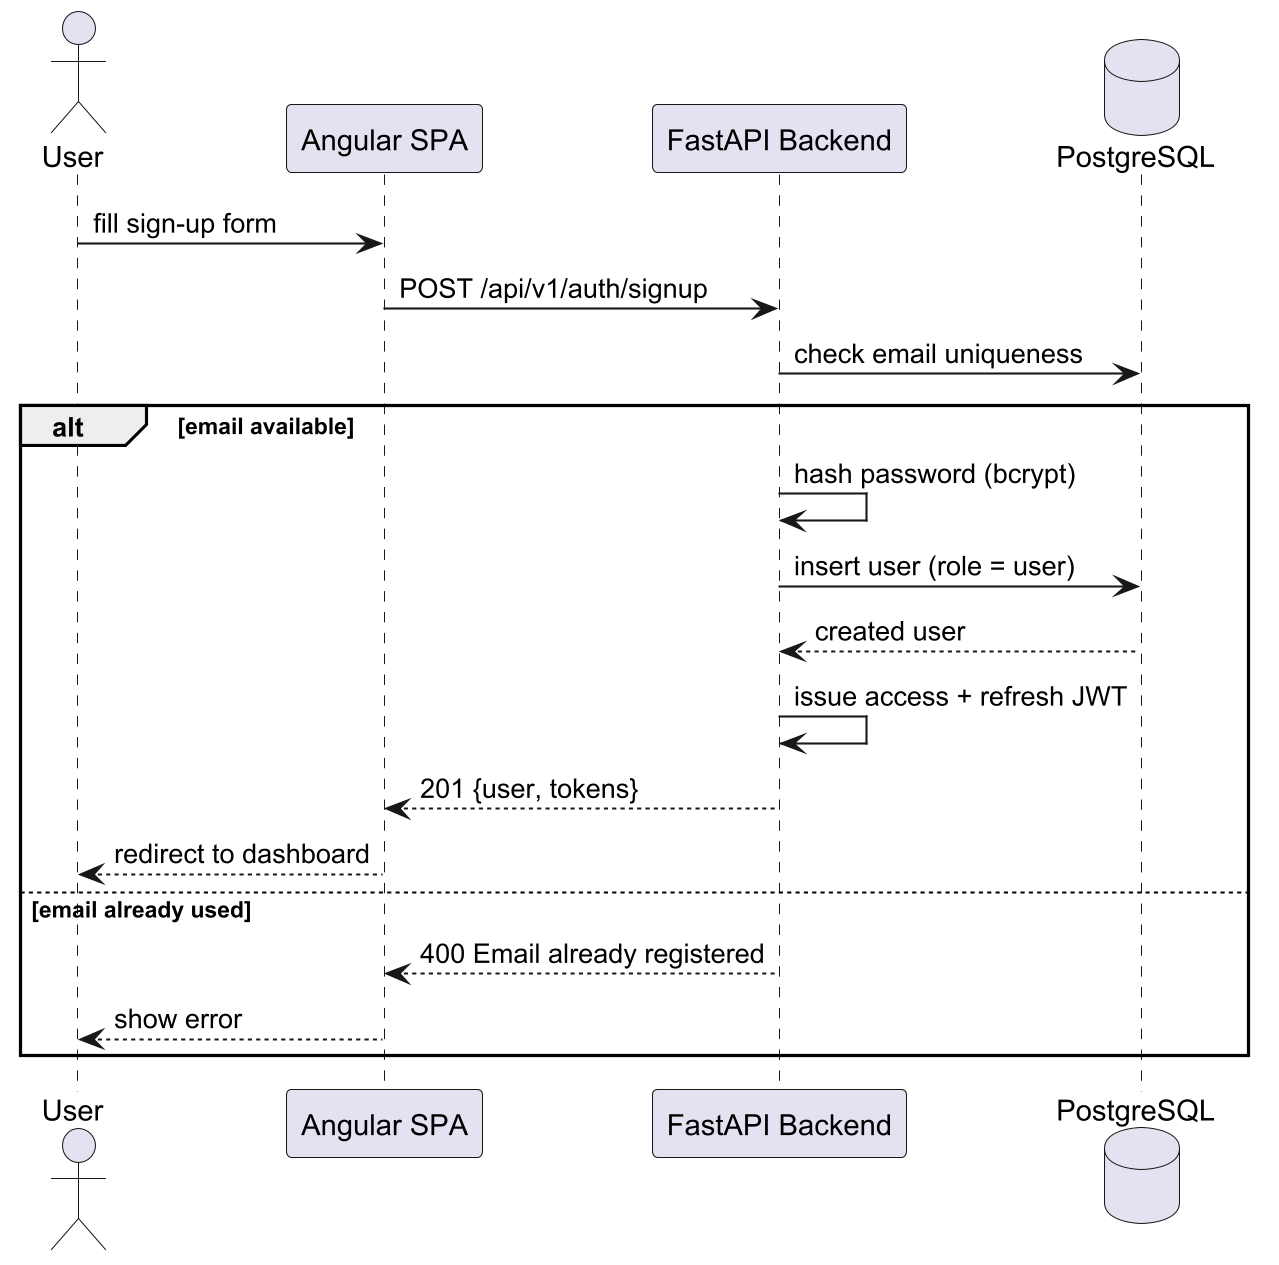
\includegraphics[width=0.92\textwidth,height=0.42\textheight,keepaspectratio]{seq_signup}
  \caption{Sequence diagram of the sign-up flow}
  \label{fig:seq-signup}
\end{figure}
\begin{figure}[H]\centering
  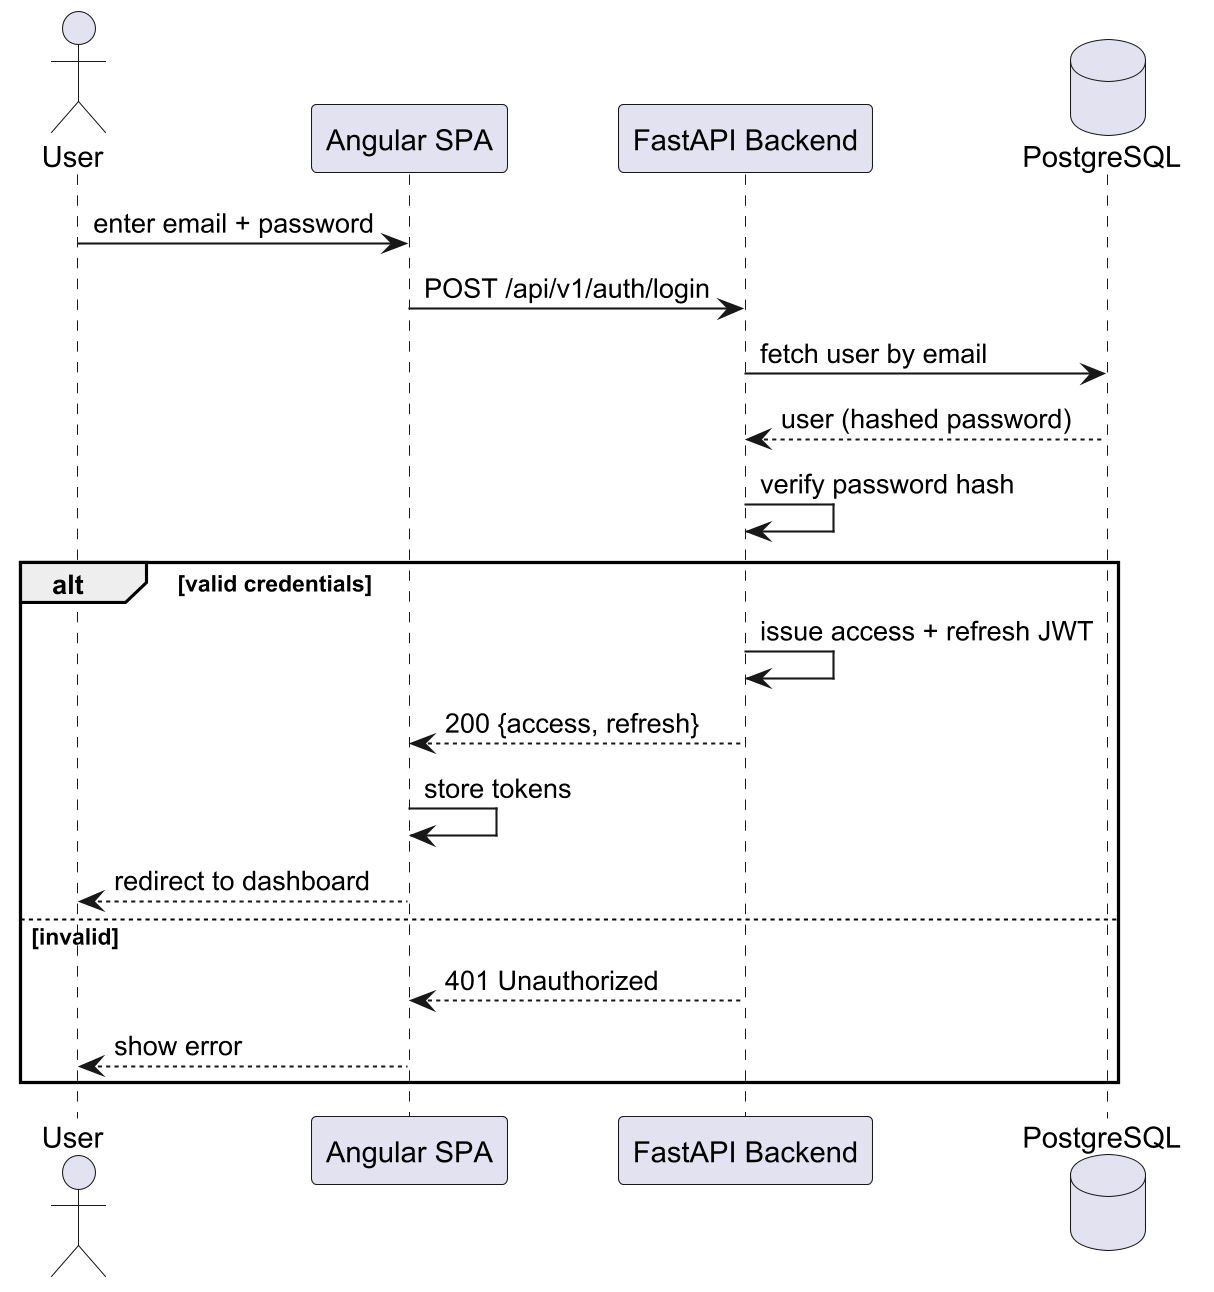
\includegraphics[width=0.92\textwidth,height=0.42\textheight,keepaspectratio]{seq_login}
  \caption{Sequence diagram of the login flow}
  \label{fig:seq-login}
\end{figure}

\subsection{Upload and Training}
Figure~\ref{fig:seq-upload} details the upload flow that feeds the pipeline,
and Figure~\ref{fig:seq-training} the training-run flow itself.
\begin{figure}[H]\centering
  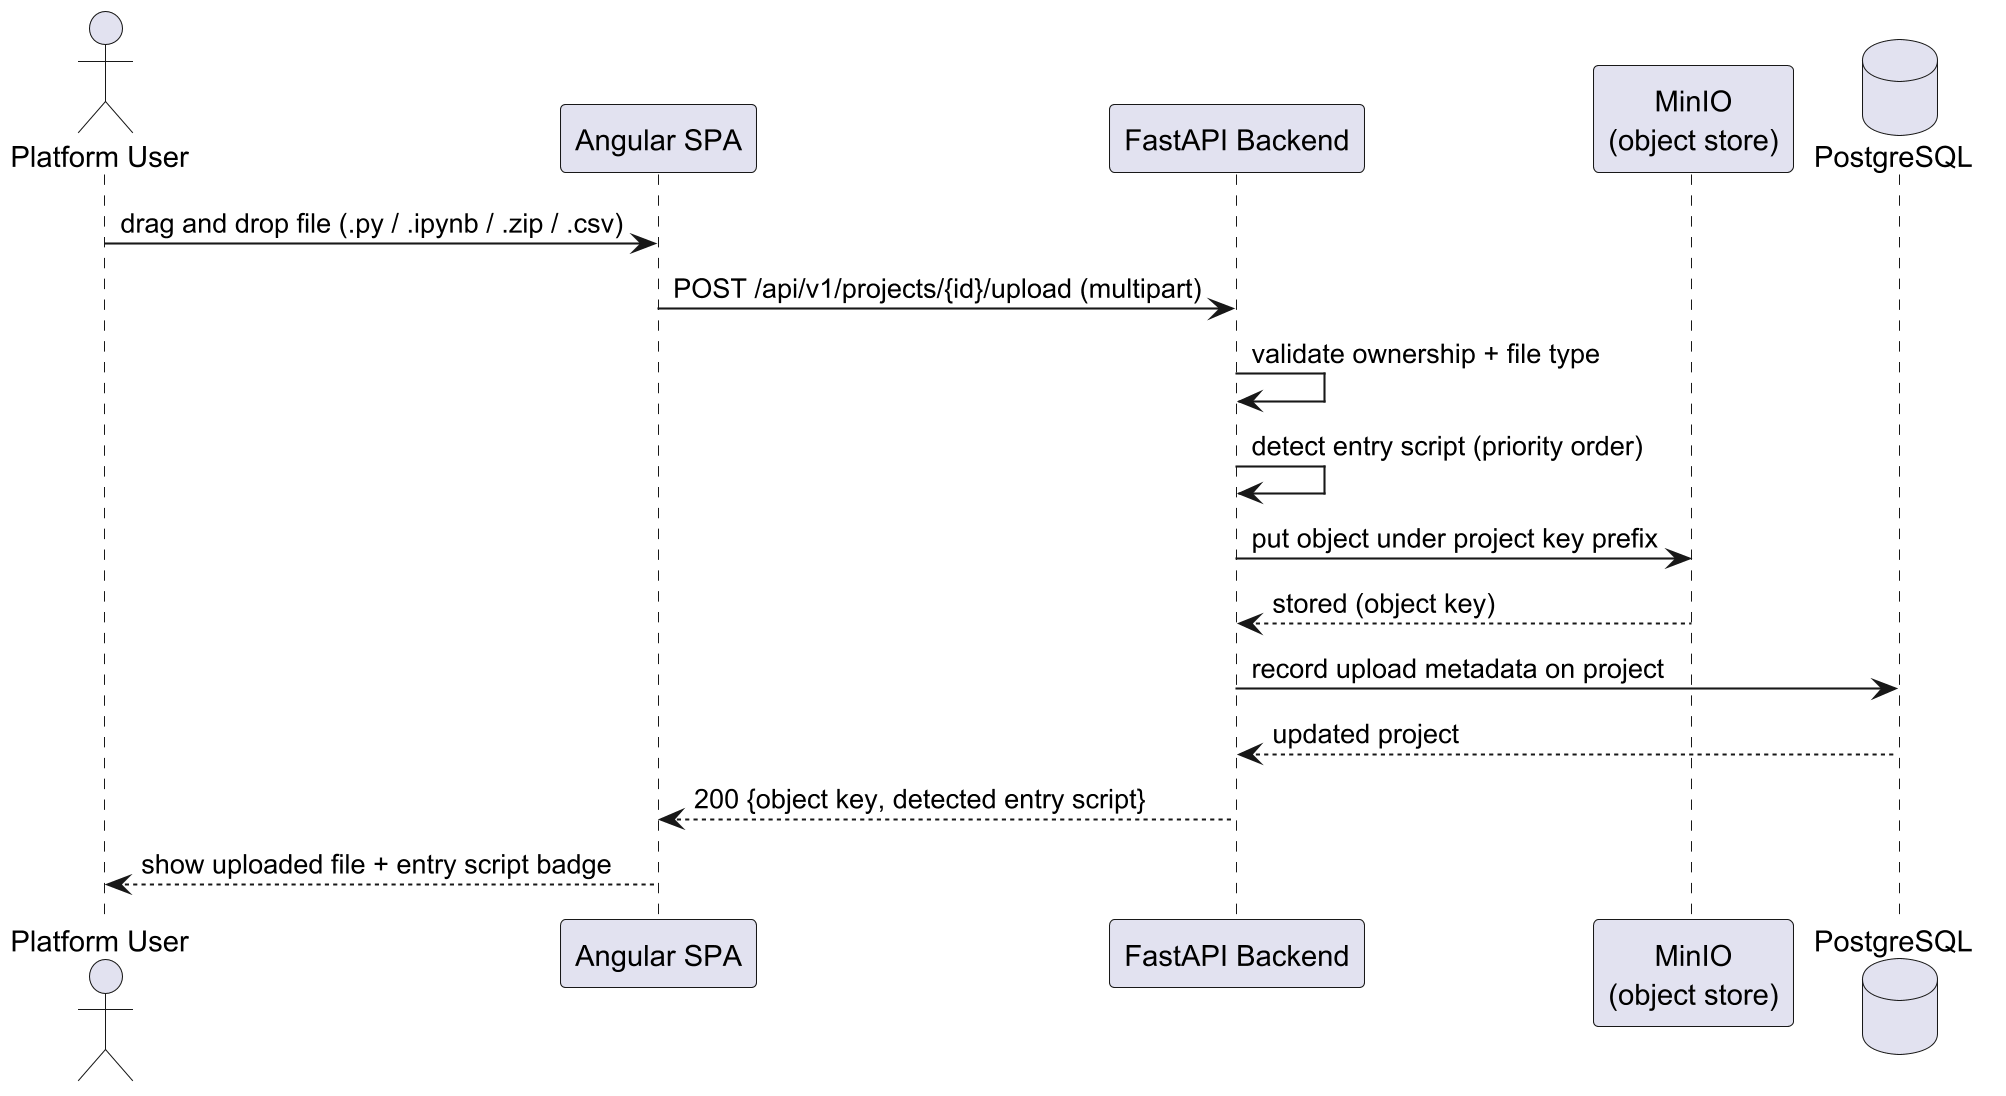
\includegraphics[width=0.92\textwidth,height=0.42\textheight,keepaspectratio]{seq_upload}
  \caption{Sequence diagram of uploading code and data to a project}
  \label{fig:seq-upload}
\end{figure}
\begin{figure}[H]\centering
  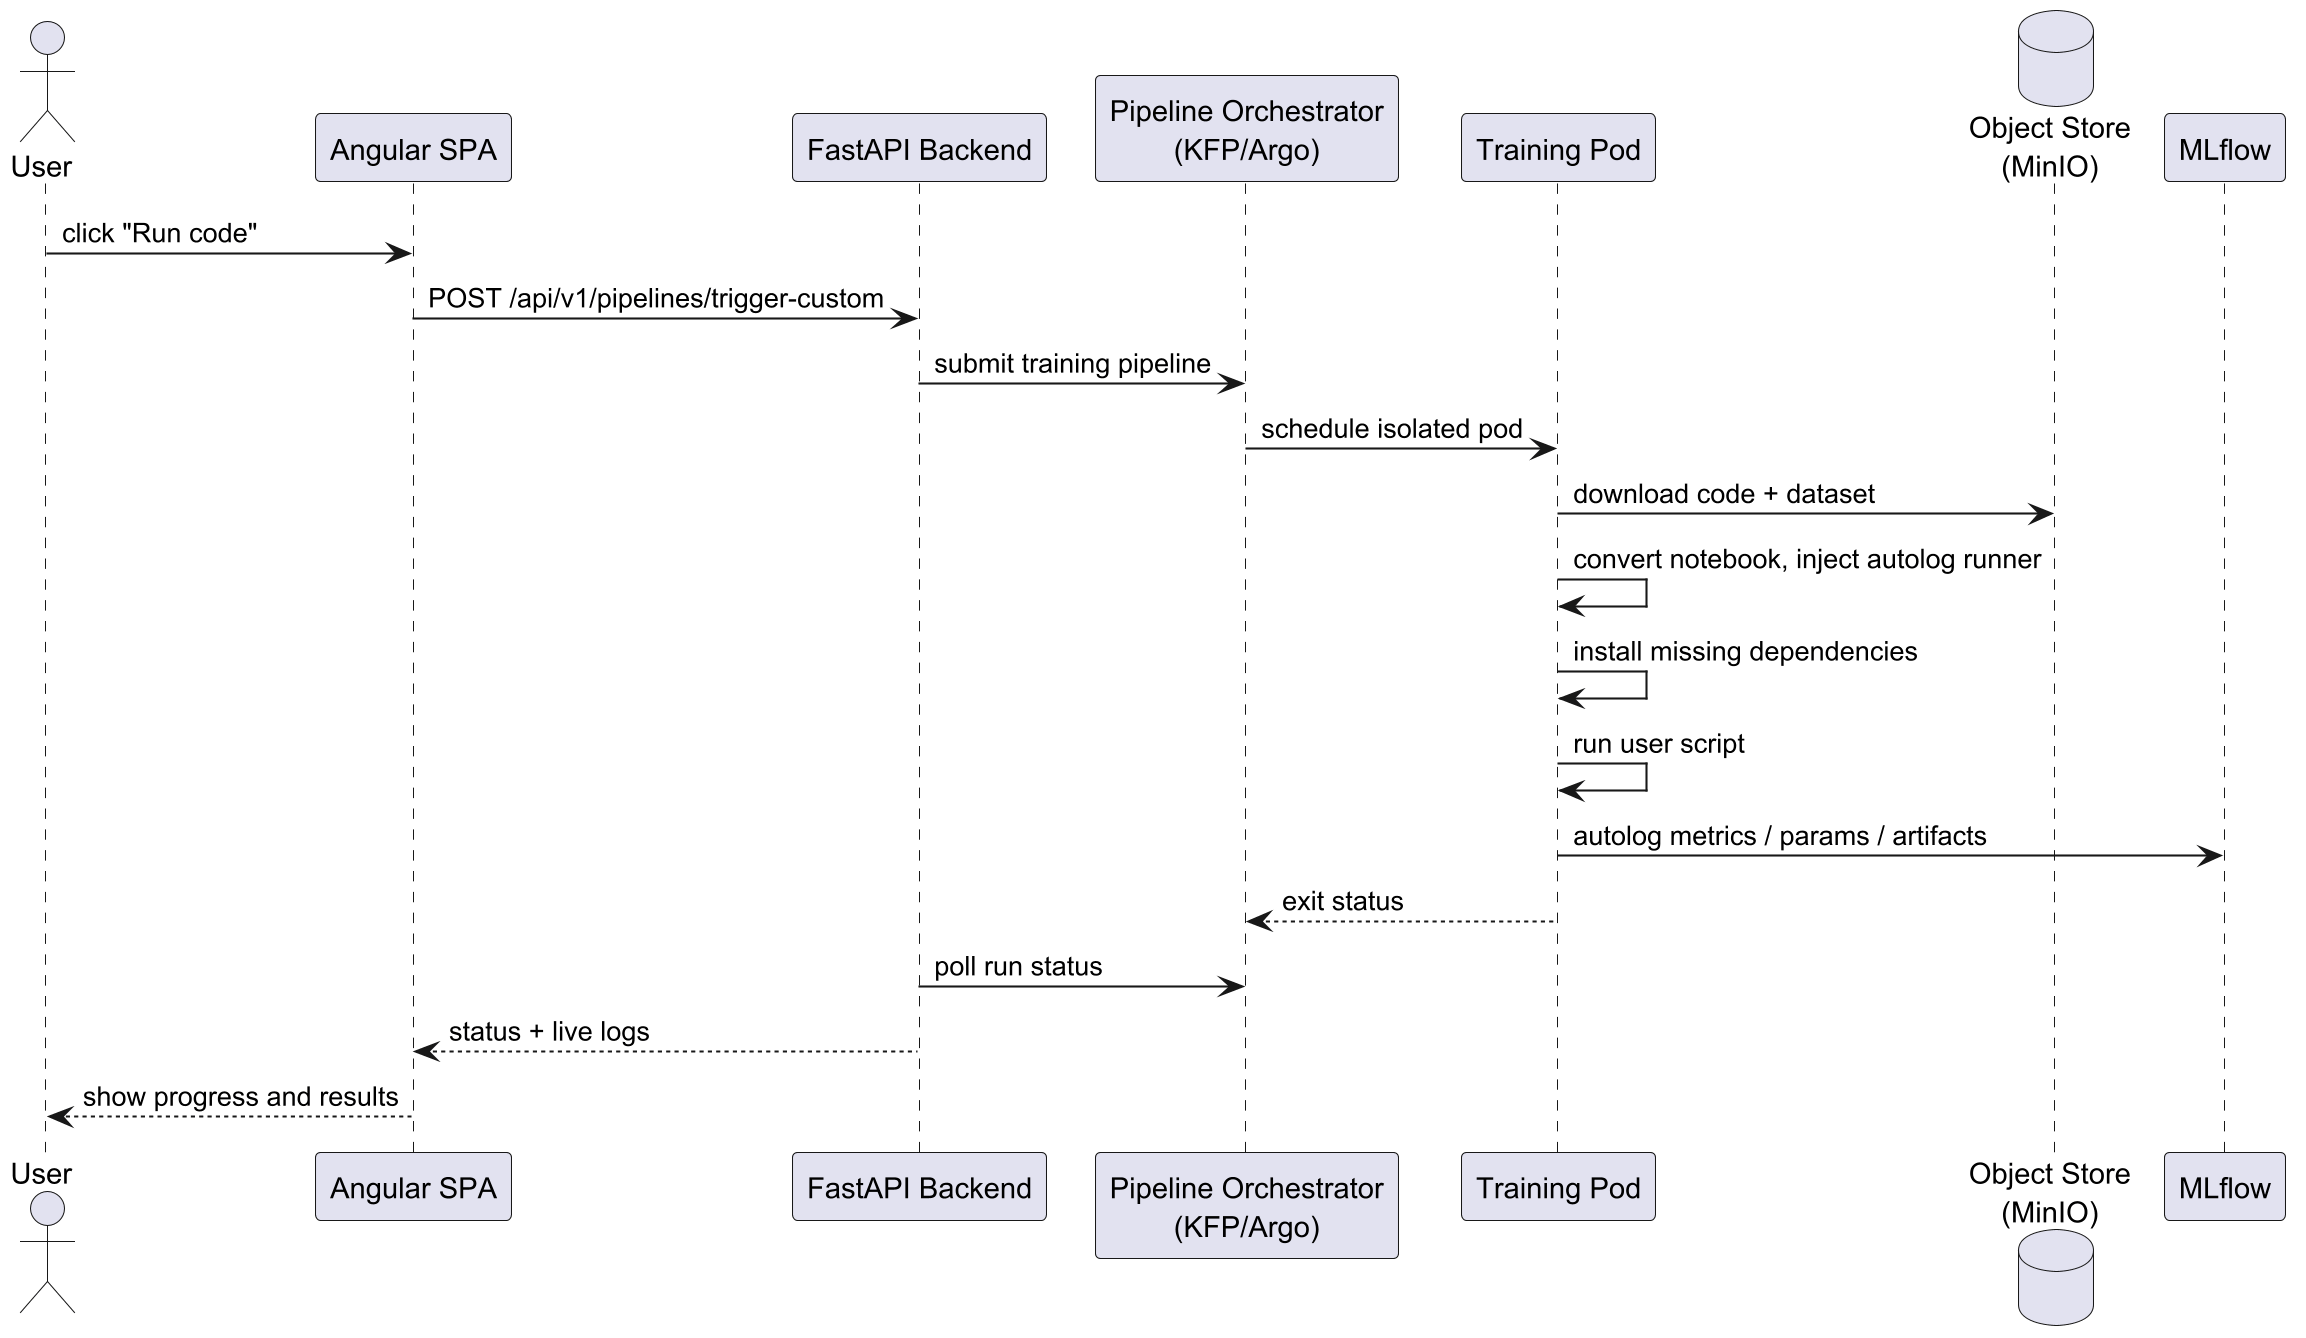
\includegraphics[width=0.92\textwidth,height=0.42\textheight,keepaspectratio]{seq_training}
  \caption{Sequence diagram of triggering a custom-code training run}
  \label{fig:seq-training}
\end{figure}

\subsection{Registry and Deployment}
Figure~\ref{fig:seq-promote} details the promotion flow, and
Figure~\ref{fig:seq-deploy} the deploy-and-predict flow.
\begin{figure}[H]\centering
  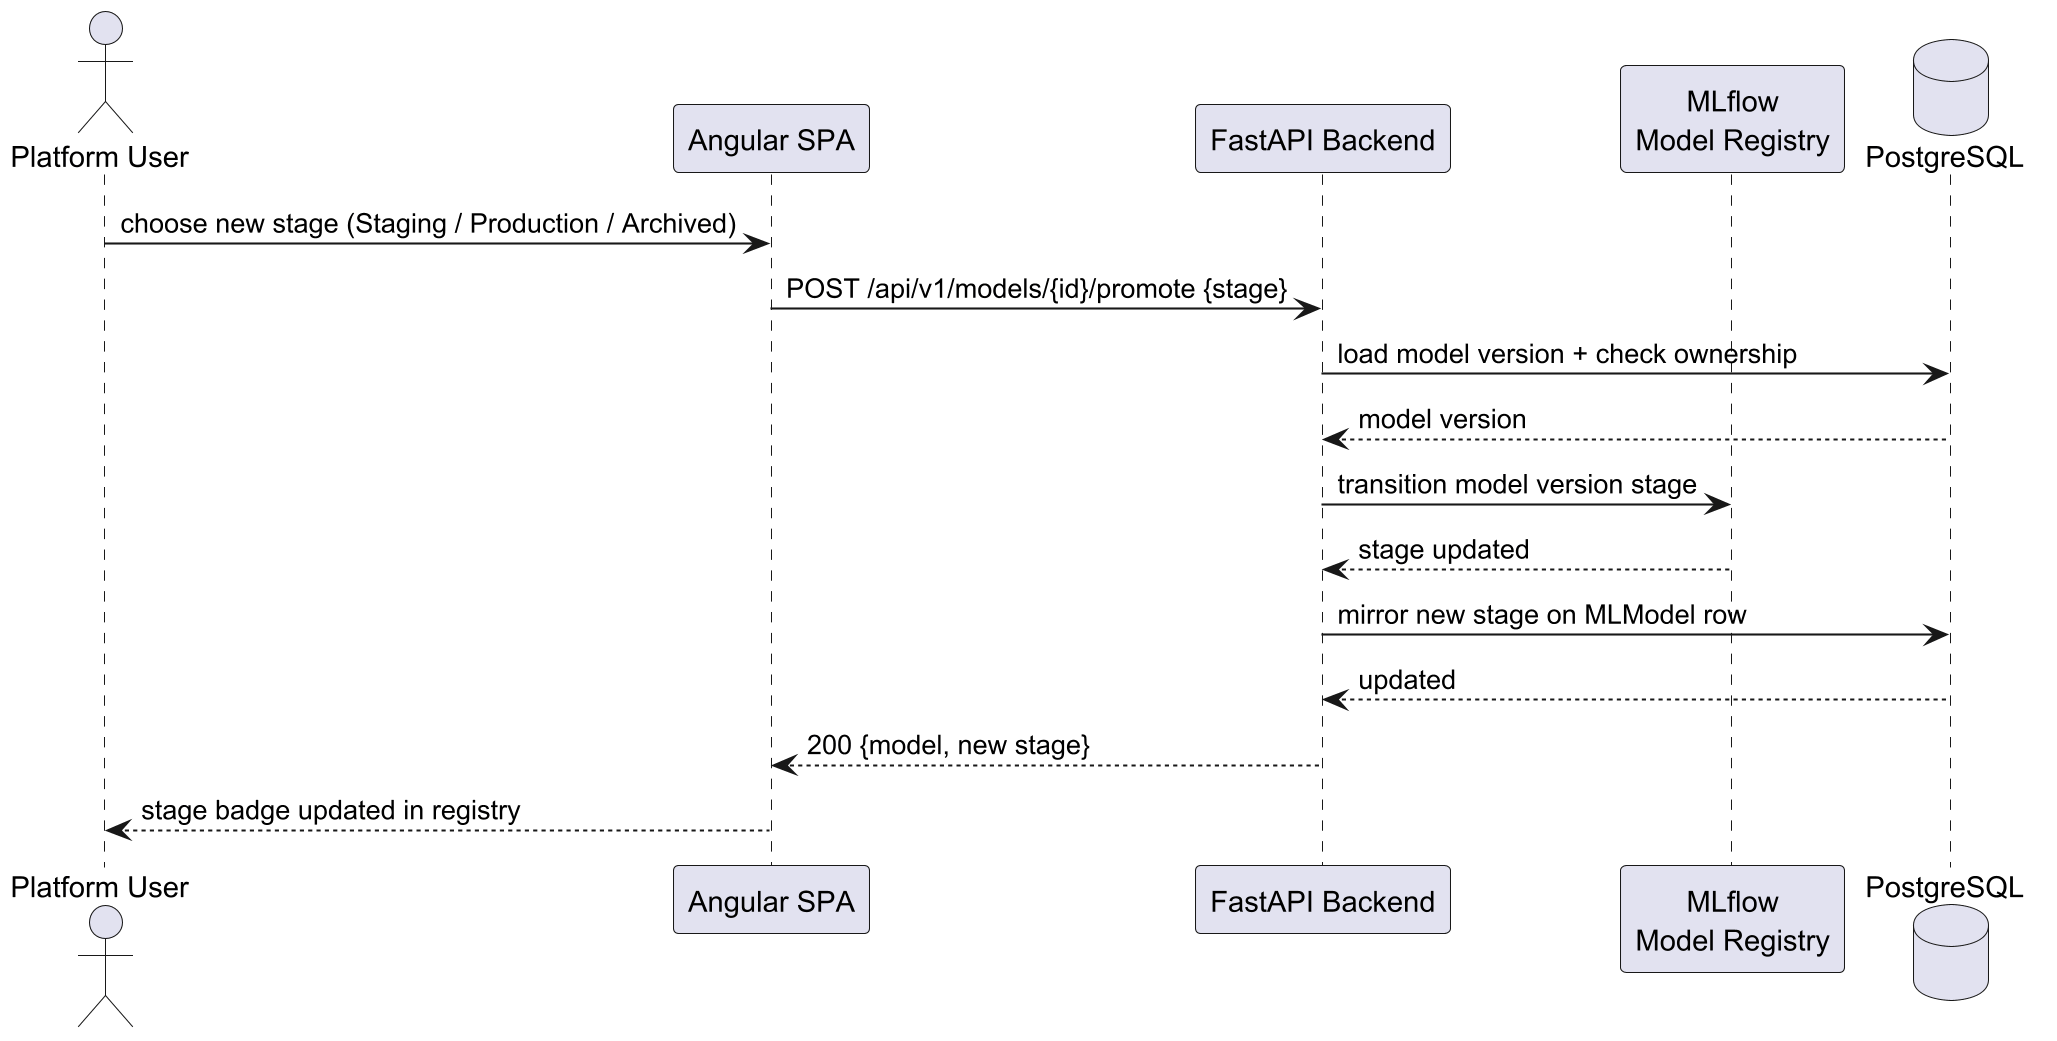
\includegraphics[width=0.92\textwidth,height=0.42\textheight,keepaspectratio]{seq_promote}
  \caption{Sequence diagram of promoting a model version}
  \label{fig:seq-promote}
\end{figure}
\begin{figure}[H]\centering
  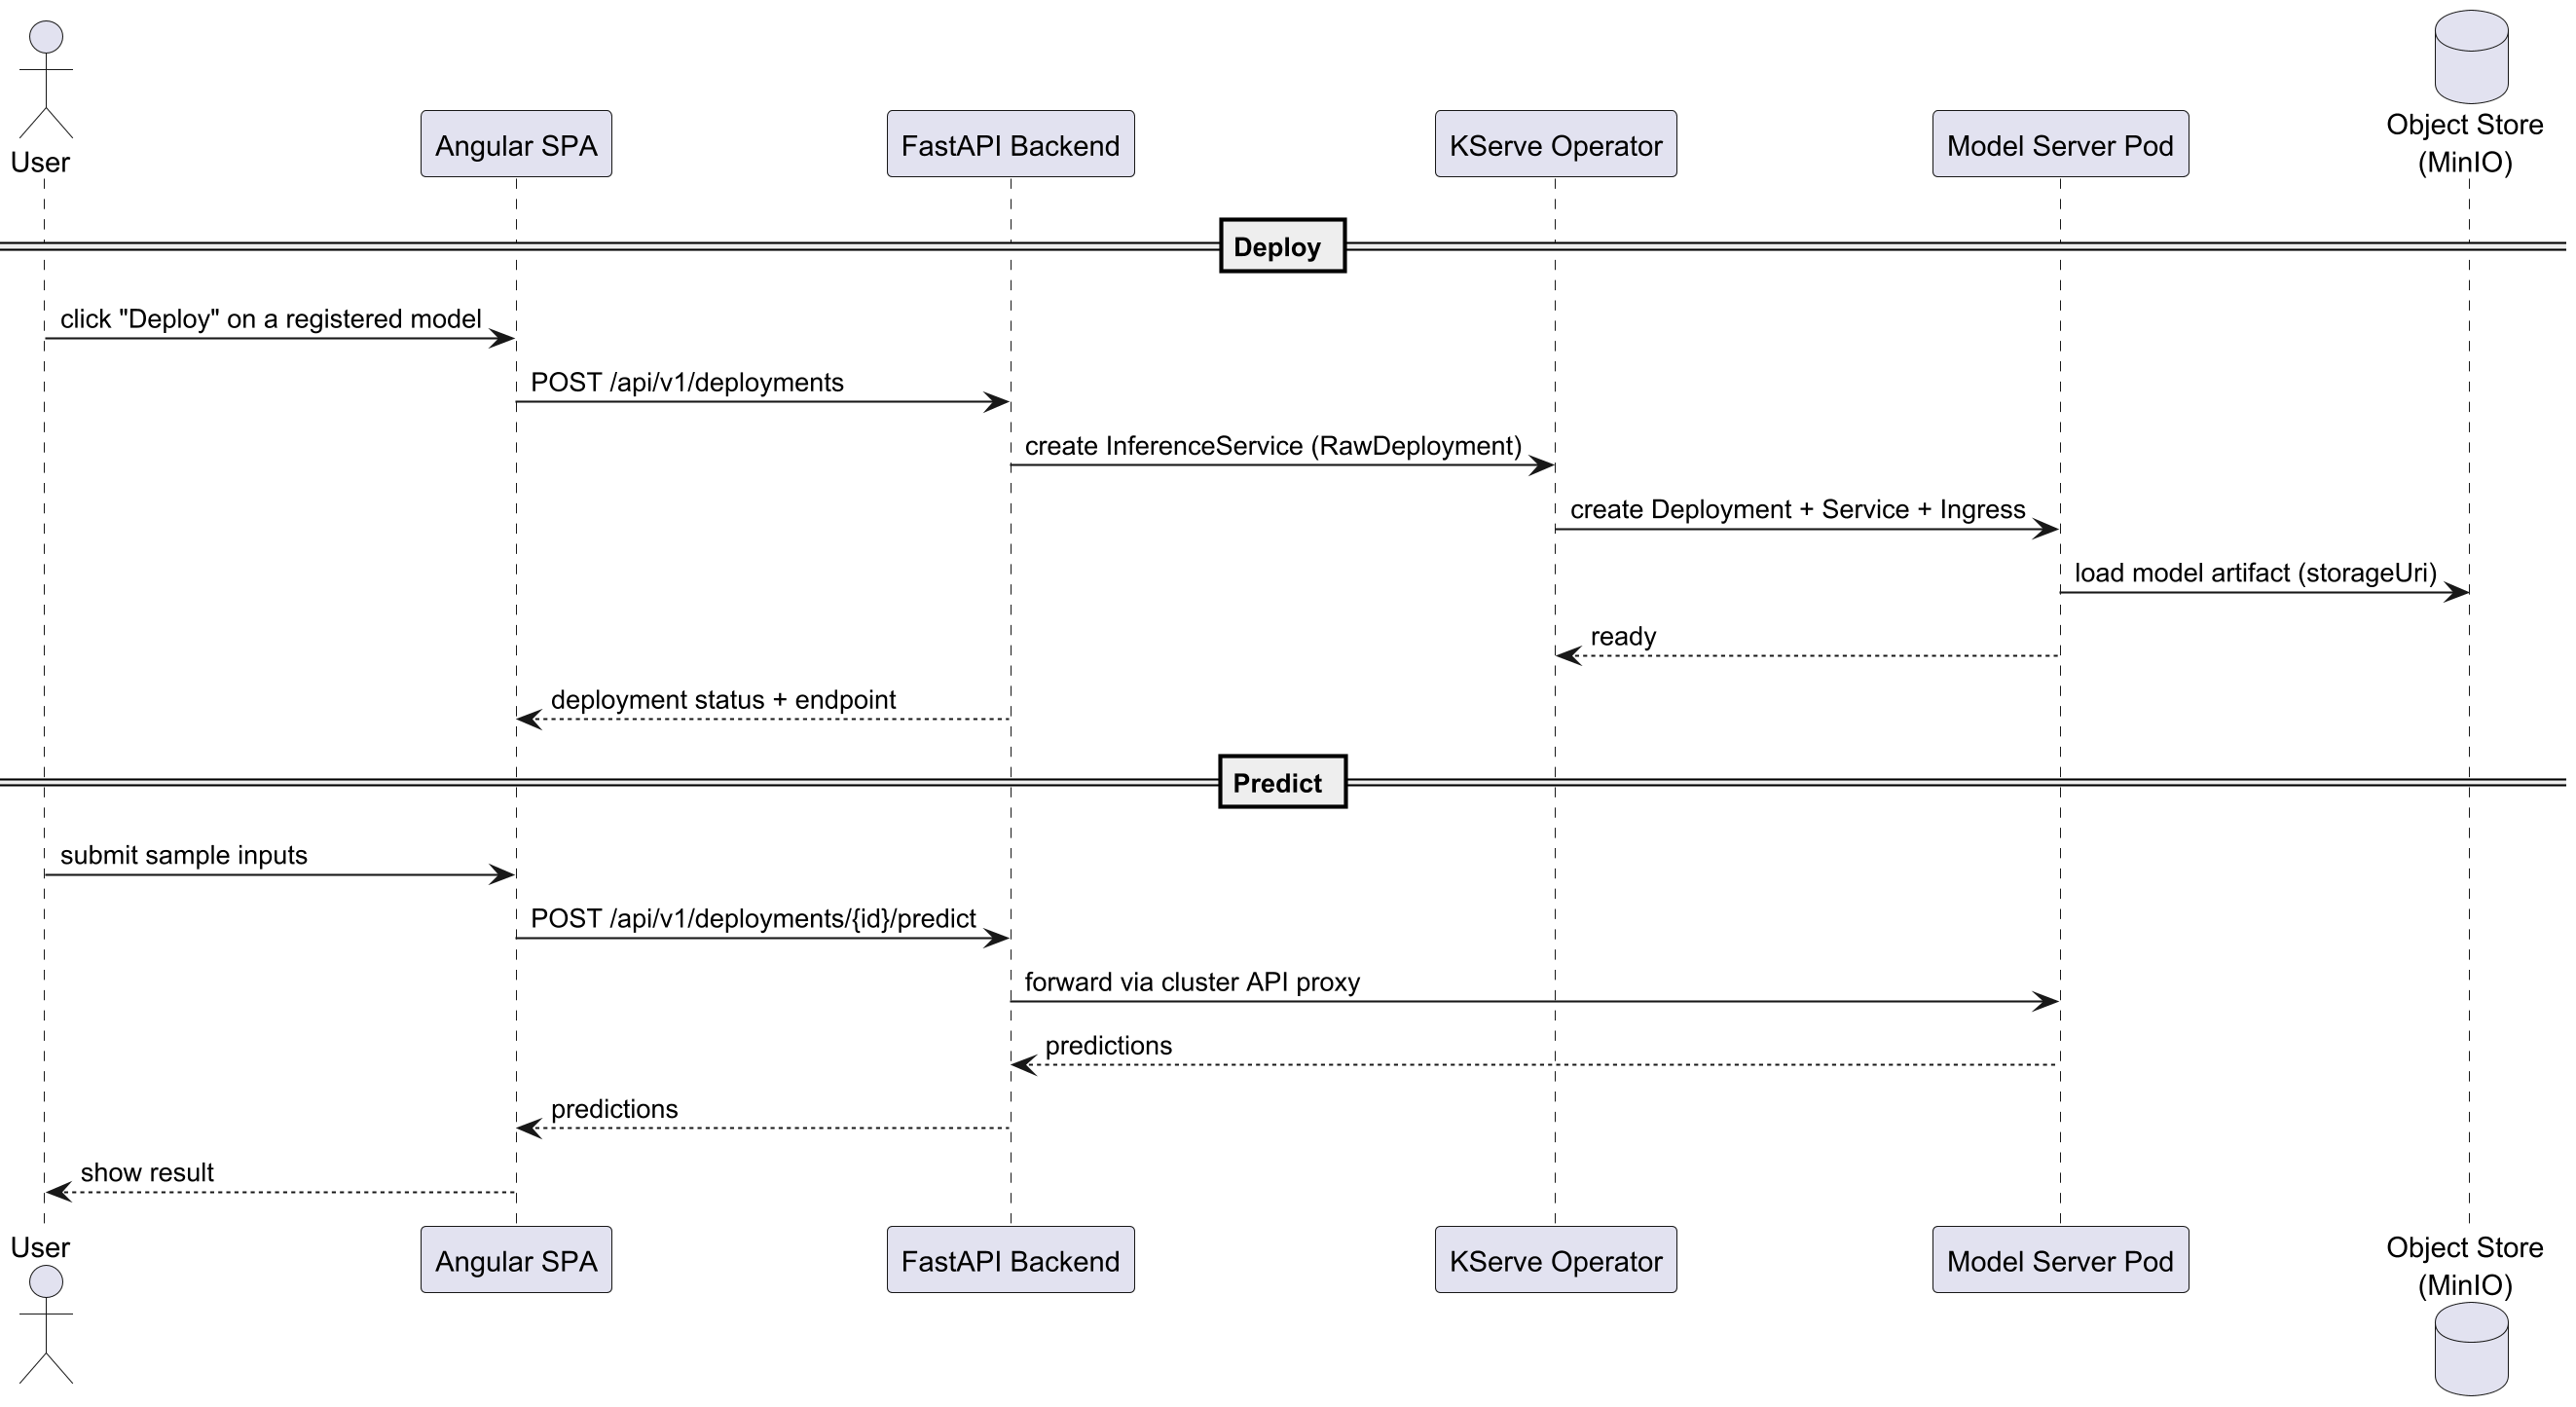
\includegraphics[width=0.92\textwidth,height=0.42\textheight,keepaspectratio]{seq_deploy}
  \caption{Sequence diagram of deploying a model and requesting a prediction}
  \label{fig:seq-deploy}
\end{figure}

\subsection{Public API and Administration}
Figure~\ref{fig:seq-public} details how an external client calls the public
endpoint, and Figure~\ref{fig:seq-admin} how an administrator manages user
accounts.
\begin{figure}[H]\centering
  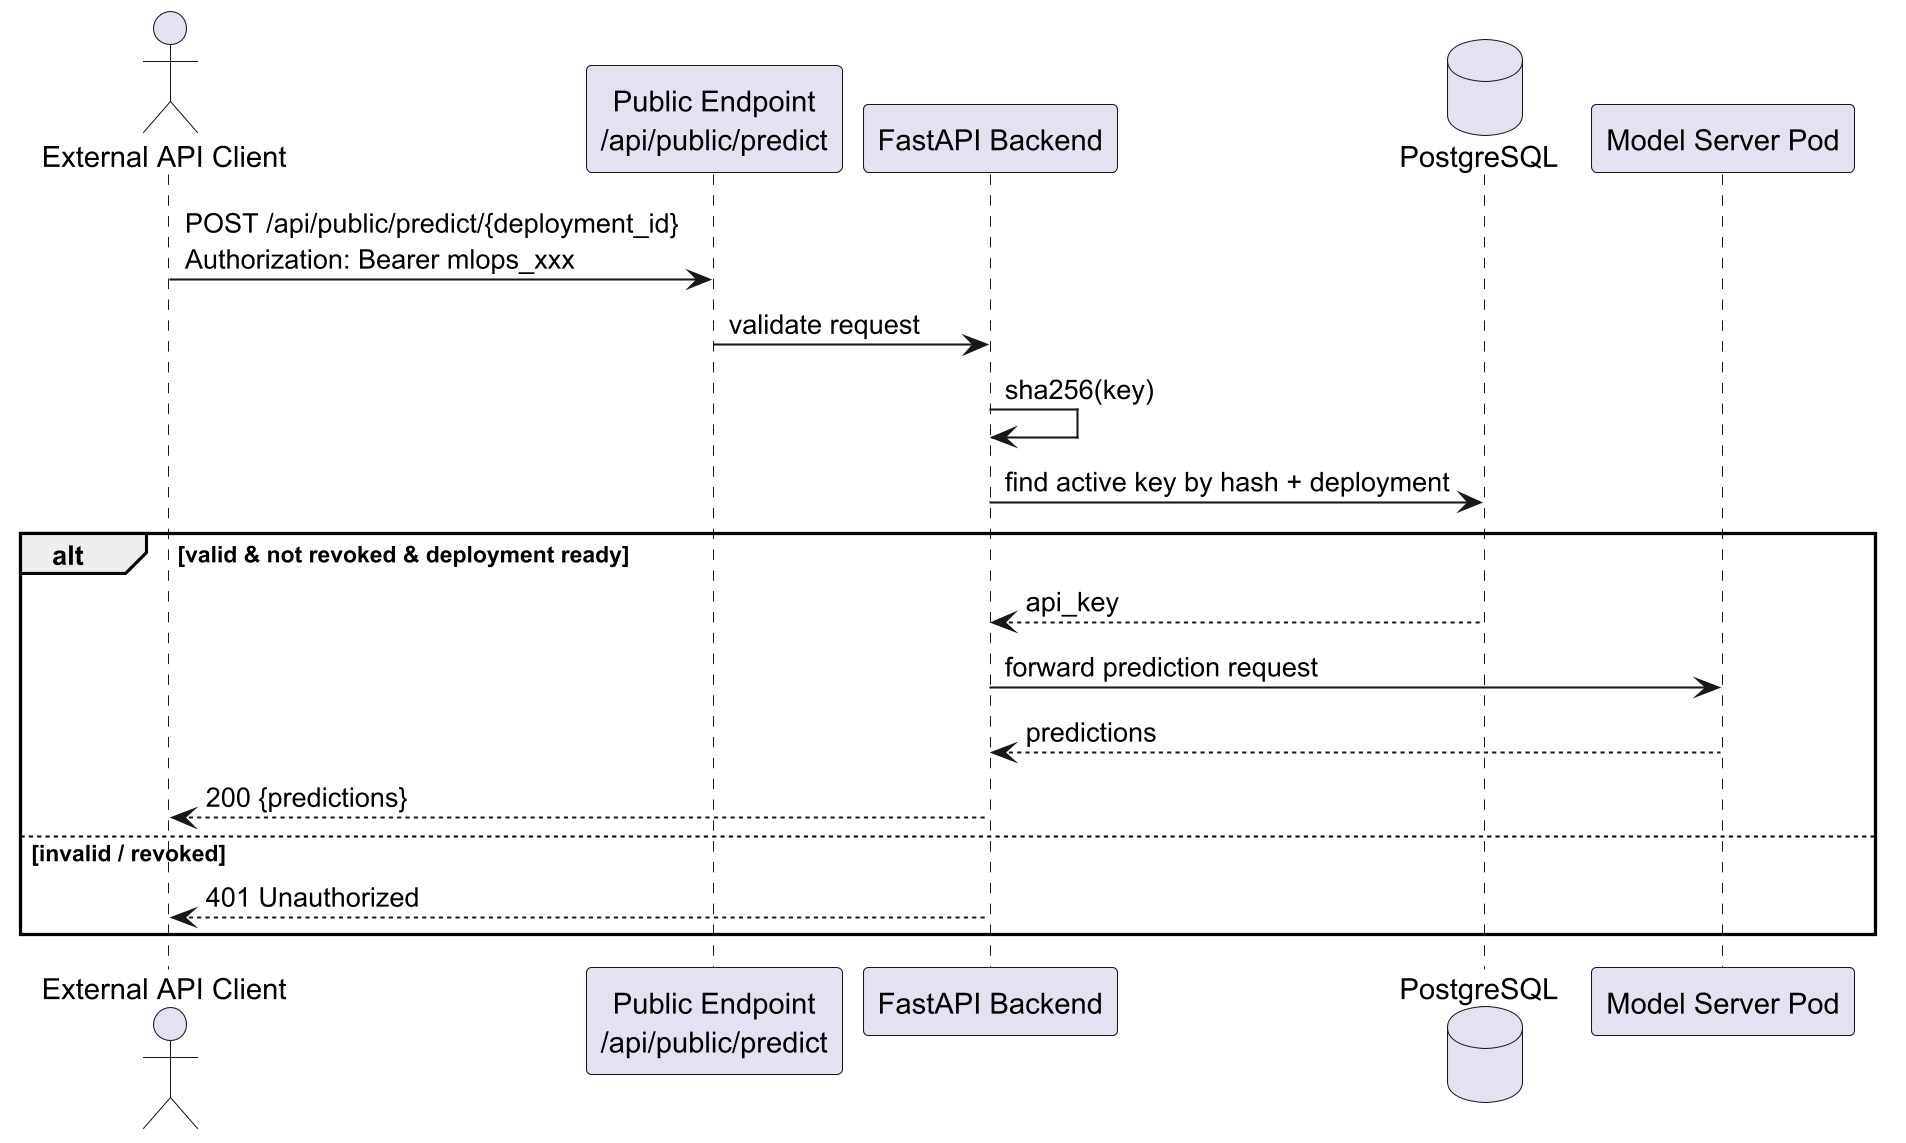
\includegraphics[width=0.92\textwidth,height=0.42\textheight,keepaspectratio]{seq_public_predict}
  \caption{Sequence diagram of an external client calling the public endpoint}
  \label{fig:seq-public}
\end{figure}
\begin{figure}[H]\centering
  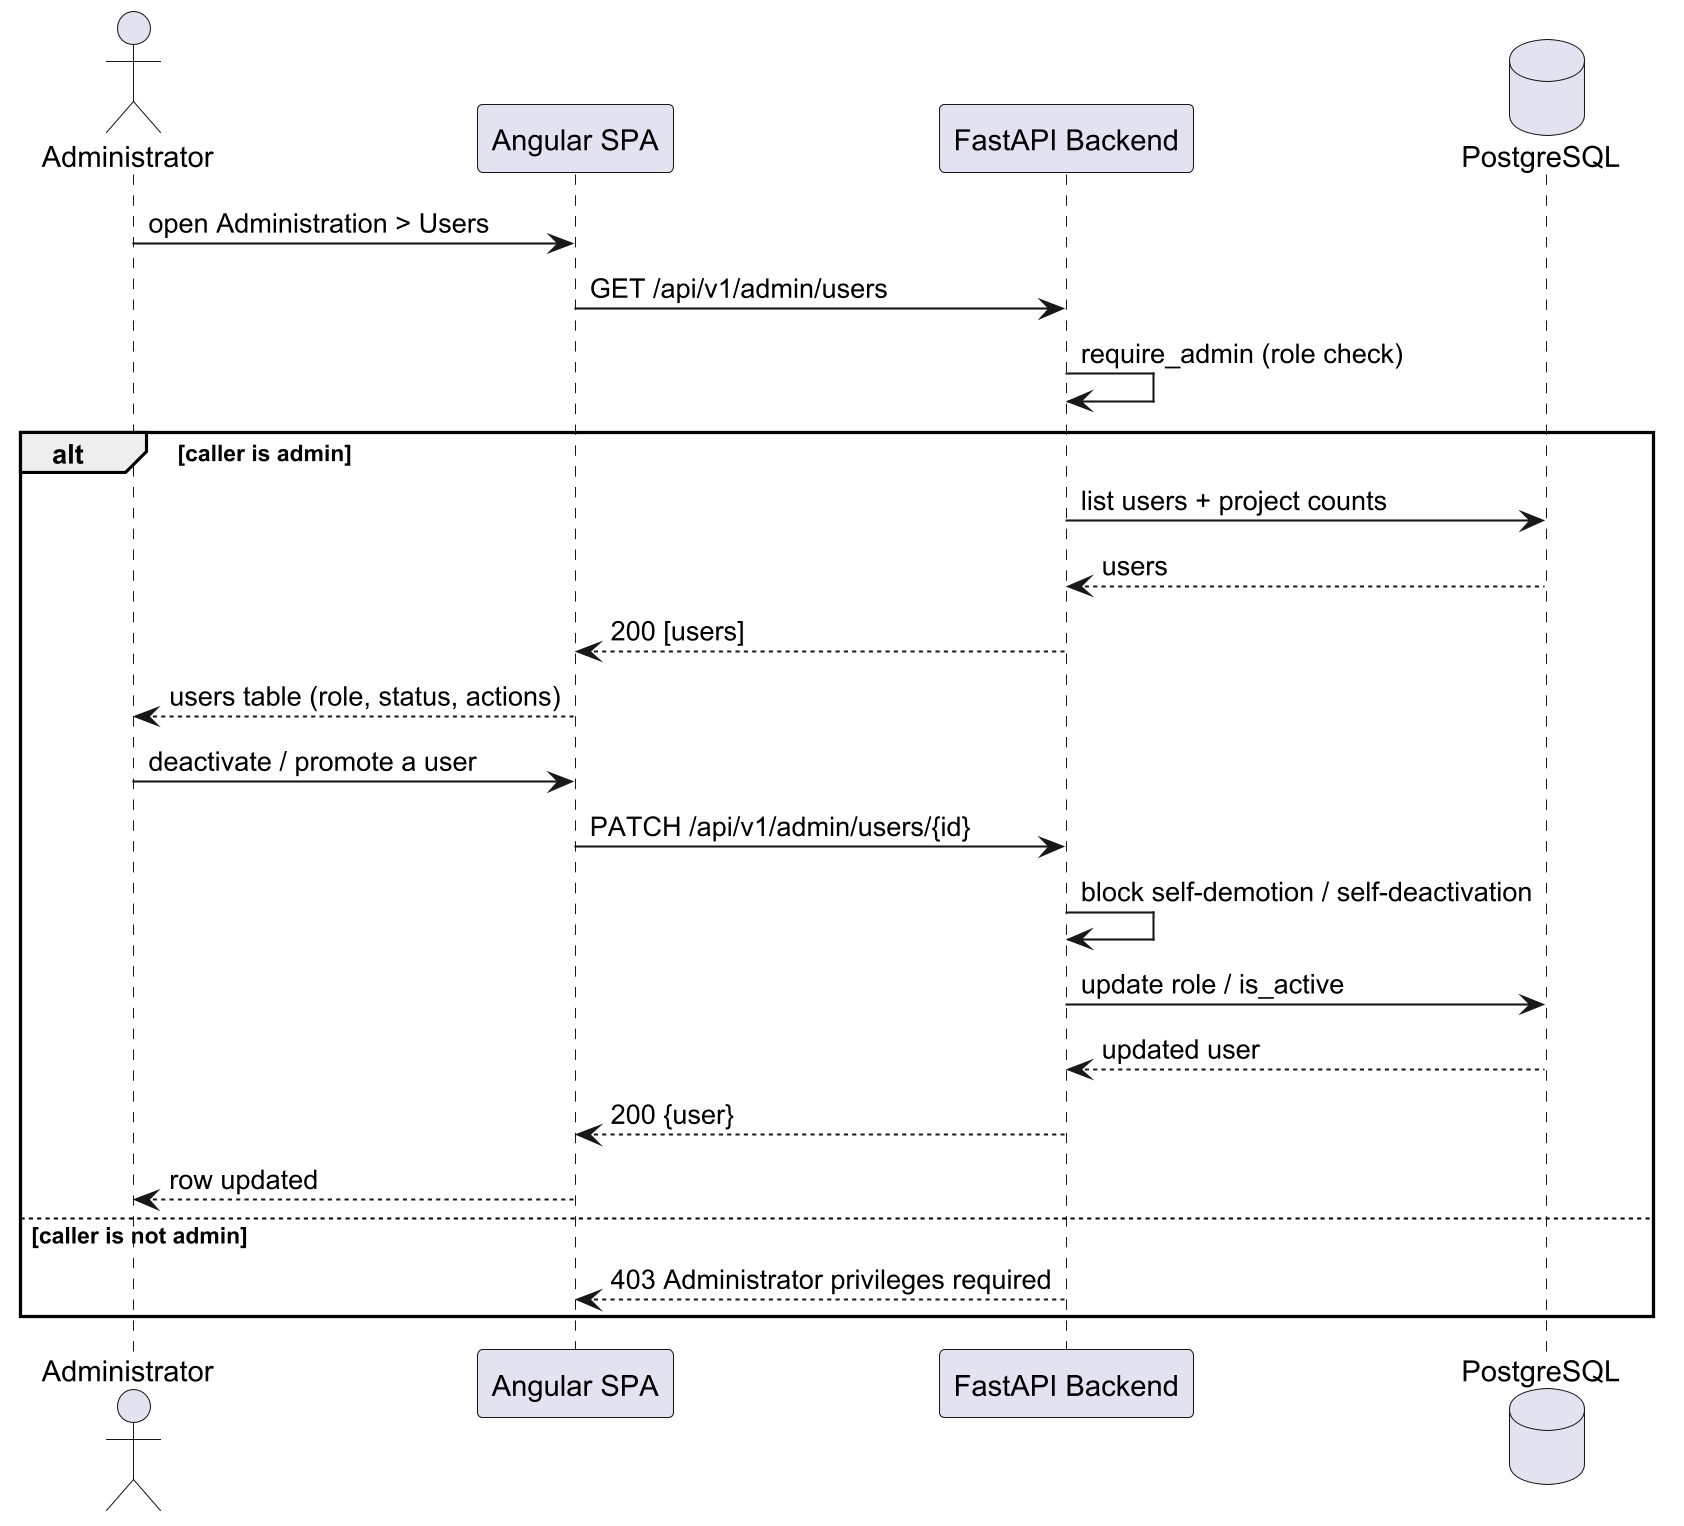
\includegraphics[width=0.92\textwidth,height=0.42\textheight,keepaspectratio]{seq_admin_users}
  \caption{Sequence diagram of administrator user management}
  \label{fig:seq-admin}
\end{figure}

% ---------------------------------------------------------------------------
\section{Data Model}
\label{sec:data-model}
The domain model is deliberately small. \texttt{User} owns \texttt{Project}; a
project accumulates \texttt{PipelineRun}s and \texttt{MLModel}s; a model can
become a \texttt{Deployment}, which owns its \texttt{DeploymentApiKey}s and
accumulates one \texttt{PredictionLog} row per served prediction. The
scientific content of a run (metrics, parameters, artifacts) deliberately
lives in the tracking server; the platform's database holds only identity,
ownership, lifecycle state, and telemetry. Figure~\ref{fig:class-global} shows
the global class diagram and Table~\ref{tab:entities} the entities with their
key attributes.

\begin{figure}[H]\centering
  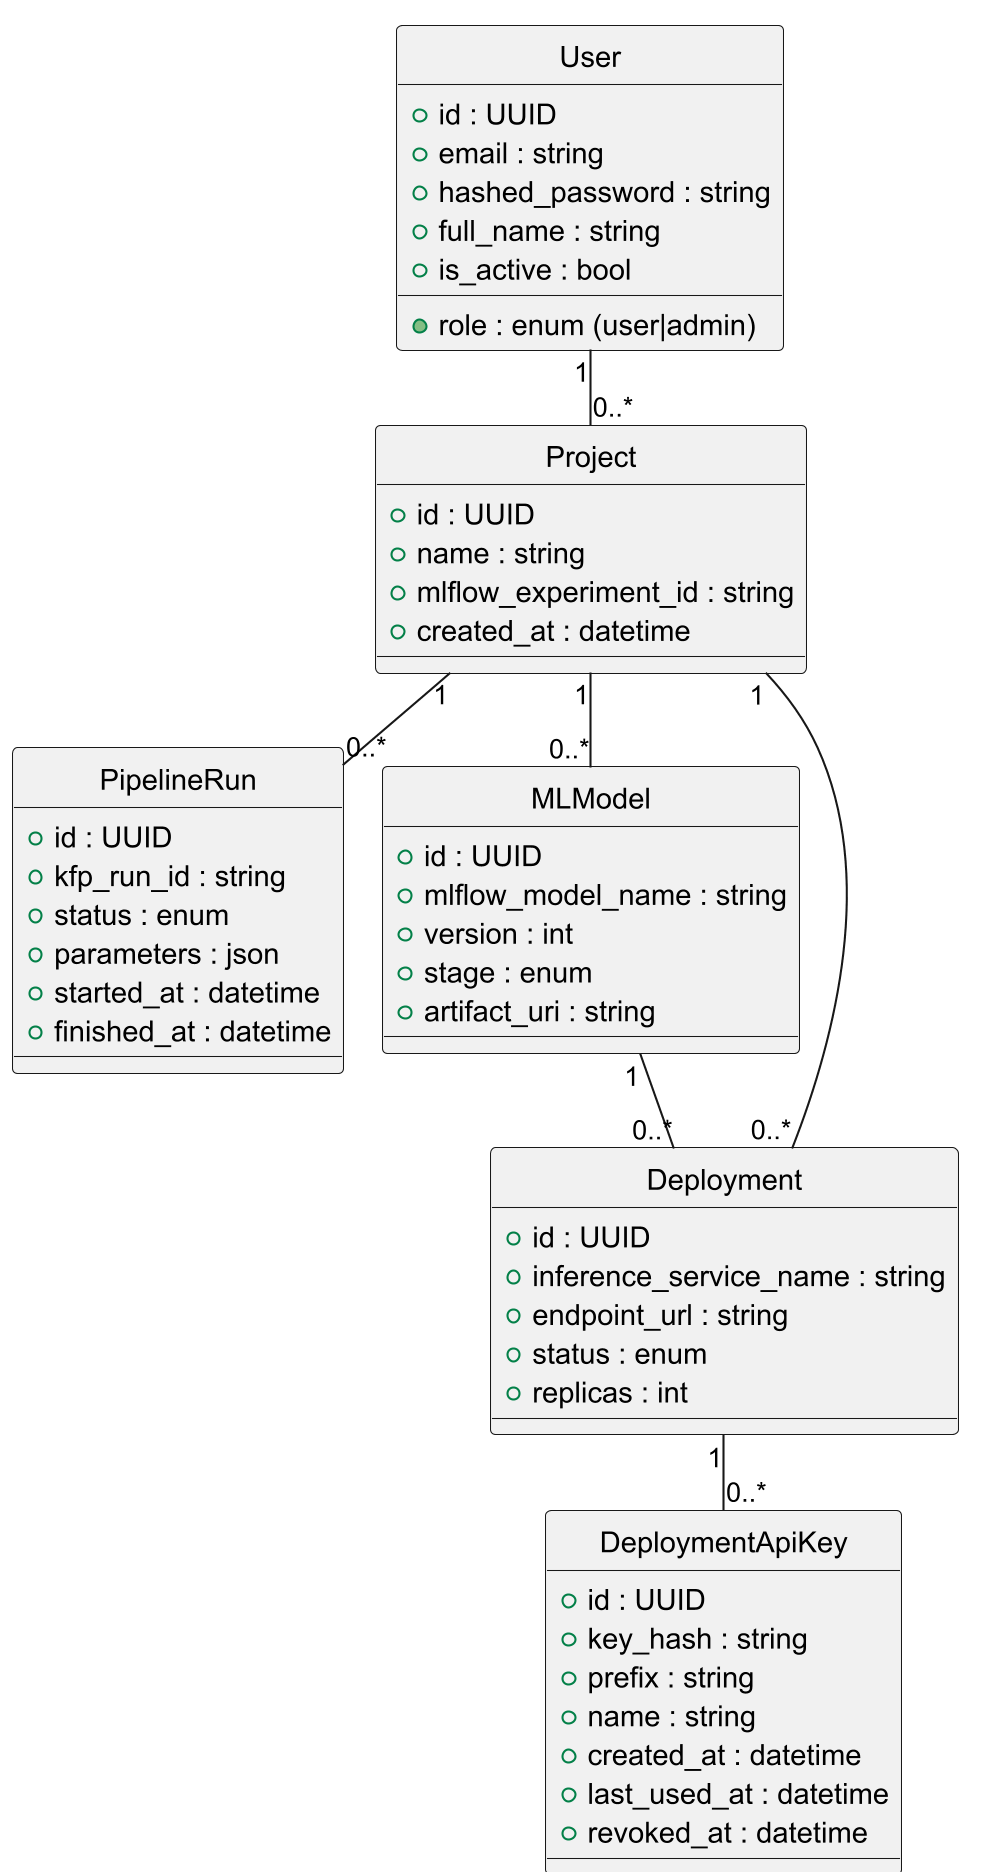
\includegraphics[width=0.95\textwidth,height=0.55\textheight,keepaspectratio]{class_domain}
  \caption{Global class diagram of the platform}
  \label{fig:class-global}
\end{figure}

\begin{table}[H]\centering
\renewcommand{\arraystretch}{1.15}
\caption{Domain entities and key attributes}\label{tab:entities}
\small
\begin{tabularx}{\textwidth}{|l|X|}
\hline
\rowcolor{primary!15}
\textbf{Entity} & \textbf{Key attributes}\\
\hline
\texttt{User} & id; unique email; bcrypt \texttt{hashed\_password}; \texttt{role} (\texttt{user}/\texttt{admin}); \texttt{is\_active}\\ \hline
\texttt{Project} & id; name, description; \texttt{owner\_id}; \texttt{experiment\_id} of its tracking experiment\\ \hline
\texttt{PipelineRun} & id; \texttt{project\_id}; \texttt{kfp\_run\_id}; status (pending/running/succeeded/failed); timestamps\\ \hline
\texttt{MLModel} & id; \texttt{project\_id}; registered name + version; stage (Staging/Production/Archived)\\ \hline
\texttt{Deployment} & id; \texttt{model\_id}; \texttt{inference\_service\_name}; status; prediction endpoint \gls{url}\\ \hline
\texttt{DeploymentApiKey} & id; \texttt{deployment\_id}; \gls{sha}-256 \texttt{key\_hash} (plaintext never stored); display prefix; \texttt{revoked\_at}\\ \hline
\texttt{PredictionLog} & id; \texttt{deployment\_id}, \texttt{project\_id}; \texttt{latency\_ms}; \texttt{status\_code}; batch size; source (app/public); indexed timestamp\\ \hline
\end{tabularx}
\end{table}

% ---------------------------------------------------------------------------
\section{Conclusion}
This chapter fixed the design of the system: four actors and their use cases,
a layered application in front of specialized cluster systems, one training
path and one serving path meeting in the object store and the registry, the
dynamic flows as sequence diagrams, and a compact domain model. The next
chapter details how this design was realized, sprint by sprint.

%==============================================================================
%  CHAPTER 4 — IMPLEMENTATION AND DEPLOYMENT
%==============================================================================
\chapter{Implementation and Deployment}
\label{chap:implementation}

\section{Introduction}
This chapter details the realization of the design of
Chapter~\ref{chap:design}, sprint by sprint, following the Scrum plan of
Chapter~\ref{chap:context}. Each sprint section presents its backlog, the key
implementation points, and the delivered interface illustrated with application
screenshots. The chapter closes with the continuous-deployment chain and the
execution environments. The validation of all delivered increments is consolidated in
Chapter~\ref{chap:validation}.

% ===========================================================================
\section{Sprint 1 --- Foundation: Identity and Projects}
\label{sec:sprint1}
The first sprint lays the groundwork: a secure authentication system and the
project entity around which all later work is organized
(Figure~\ref{fig:sprint1-strip}).

\begin{figure}[H]\centering
  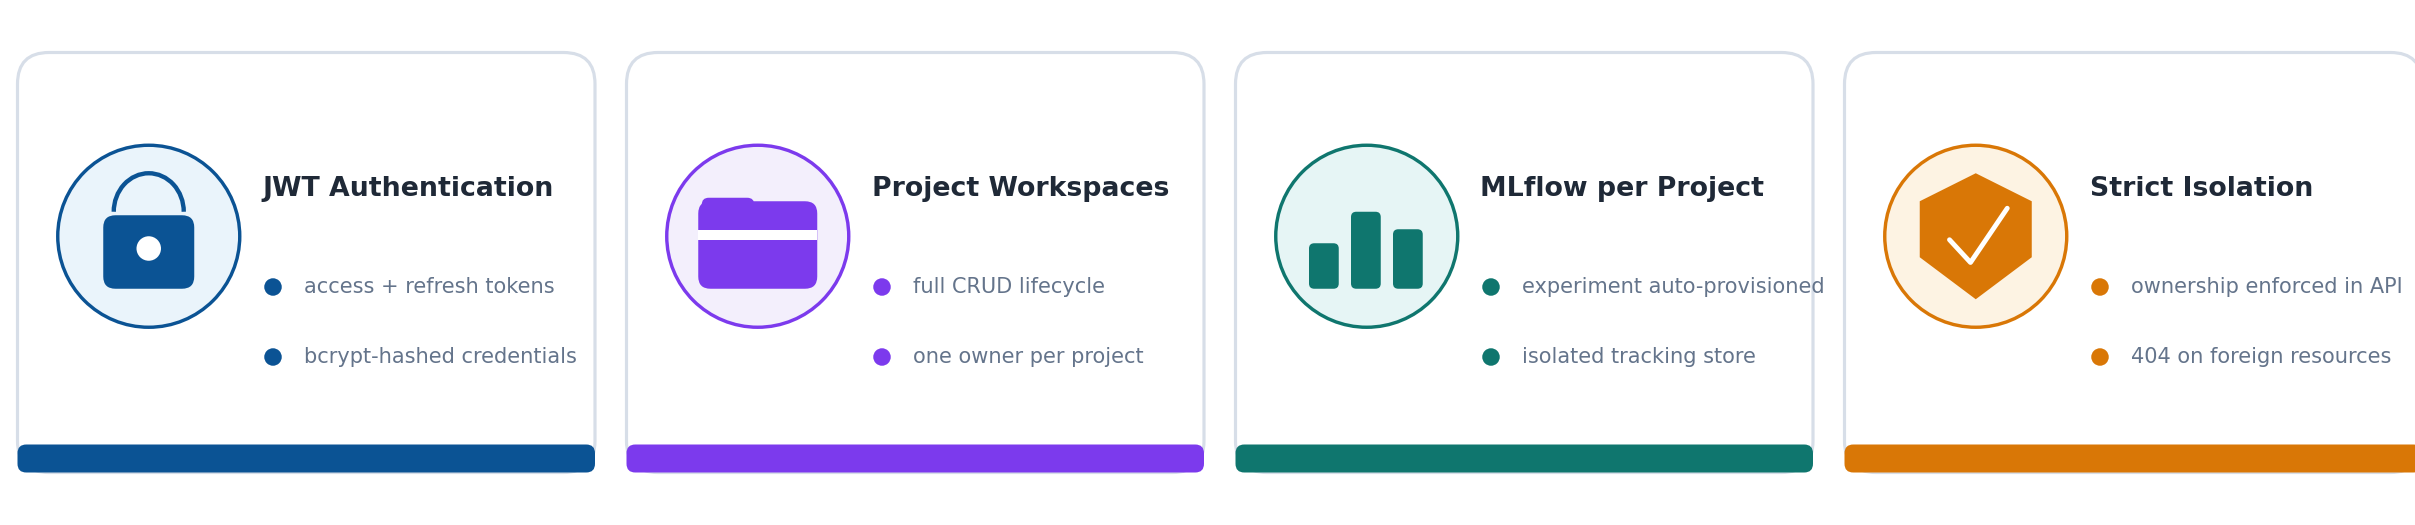
\includegraphics[width=\textwidth,keepaspectratio]{sprint1_features}
  \caption{Sprint 1 at a glance: authentication, projects, isolation}
  \label{fig:sprint1-strip}
\end{figure}

\begin{table}[H]\centering
\renewcommand{\arraystretch}{1.15}
\caption{Sprint~1 backlog}\label{tab:backlog-s1}
\small
\begin{tabularx}{\textwidth}{|c|X|c|}
\hline
\rowcolor{primary!15}
\textbf{\#} & \textbf{Task} & \textbf{Pts}\\
\hline
1 & Design the user and project data model & 2\\ \hline
1 & Implement signup / login / refresh with JWT & 3\\ \hline
1 & Build the login and signup user interface & 1\\ \hline
2 & Implement project CRUD with ownership checks & 2\\ \hline
2 & Bind each project to its own tracking experiment & 1\\ \hline
2 & Build the projects list and detail interface & 1\\ \hline
\end{tabularx}
\end{table}

\subsection{Authentication with JWT}
Authentication is stateless and based on \gls{jwt}. On login, the backend
verifies the password against its stored bcrypt hash and issues a short-lived
\emph{access} token and a longer-lived \emph{refresh} token. Protected
endpoints depend on a function that decodes the token and resolves the current
user; the refresh endpoint renews the session without re-entering credentials
(Figure~\ref{fig:screen_login}).

\bigshot{screen_login}{The authentication screen}{A returning user signs in
with email and password; new users switch to the sign-up form, and sessions
are kept alive transparently through the refresh token.}

\subsection{Project Management and Isolation}
A project is the organizing unit of the platform. Creating one also provisions
a dedicated experiment in the tracking server, so every run under the project
is grouped automatically. All project endpoints enforce an ownership check
that answers \texttt{404}, not \texttt{403}, for foreign resources: another
user's project simply does not exist for the caller. The frontend mirrors this
protection with an Angular route guard that redirects any unauthenticated
access to the login page (Figure~\ref{fig:screen_projects}).

\bigshot{screen_projects}{The projects workspace}{Each card is an isolated
project bound to its own tracking experiment, and the dialog creates a new
project; a user only ever sees the projects they own.}

\subsection{Sprint Review}
The increment was demonstrated to the supervisors and accepted: accounts,
sessions, and isolated project workspaces worked end to end on the cluster.
The retrospective confirmed the choice of stateless \gls{jwt} sessions and led
to one adjustment: answering \texttt{404} instead of \texttt{403} on foreign
resources, so that ownership is never leaked.

% ===========================================================================
\section{Sprint 2 --- Training and Tracking: the Engine}
\label{sec:sprint2}
The second sprint delivers the heart of the platform: uploading code and data,
running it as an isolated job on the cluster, and capturing the results
automatically (Figure~\ref{fig:sprint2-strip}).

\begin{figure}[H]\centering
  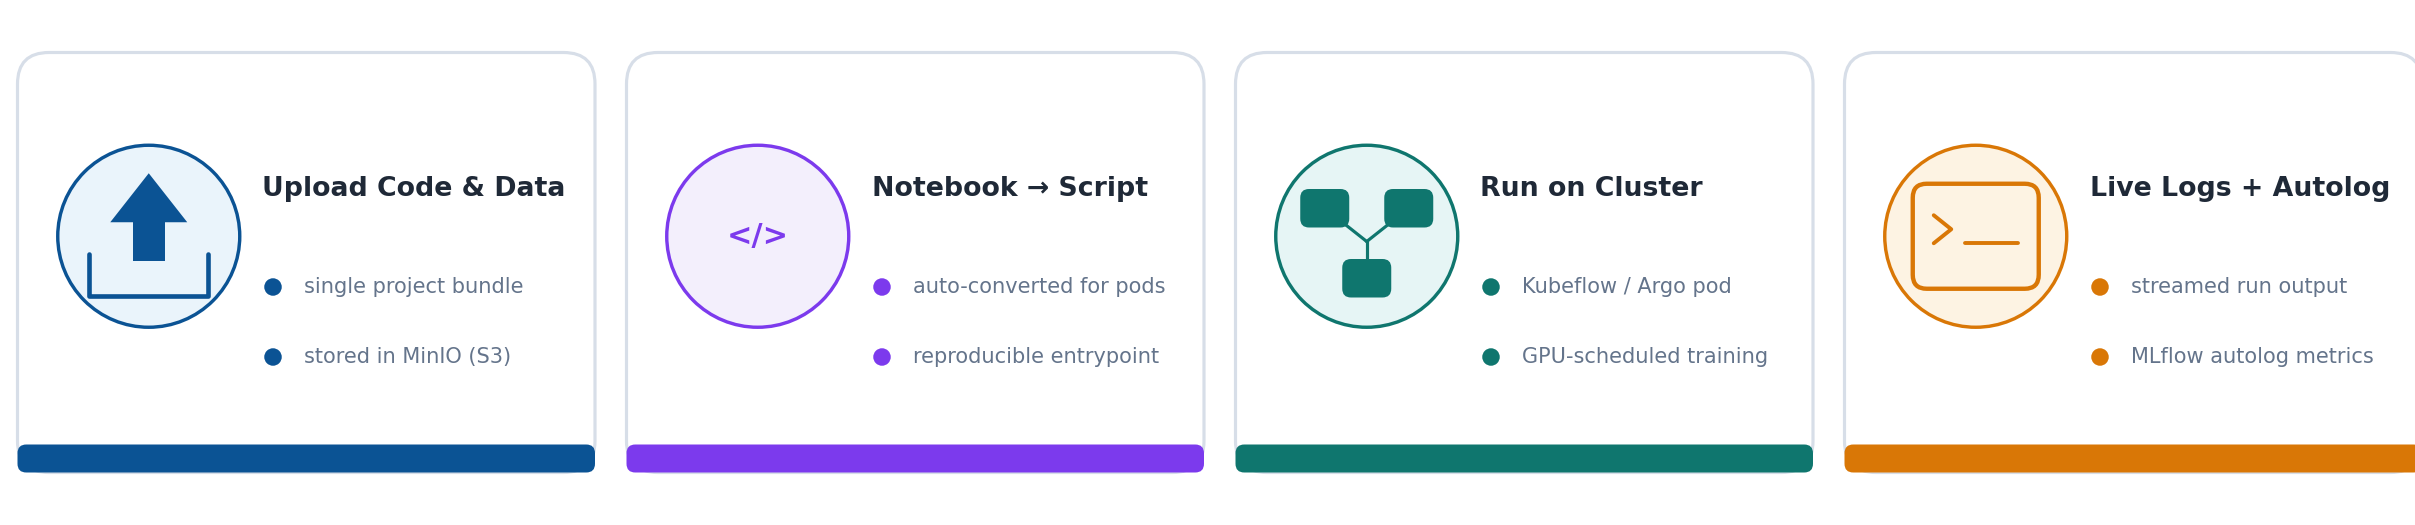
\includegraphics[width=\textwidth,keepaspectratio]{sprint2_features}
  \caption{Sprint 2 at a glance: upload, conversion, cluster runs, live logs}
  \label{fig:sprint2-strip}
\end{figure}

\begin{table}[H]\centering
\renewcommand{\arraystretch}{1.15}
\caption{Sprint~2 backlog}\label{tab:backlog-s2}
\small
\begin{tabularx}{\textwidth}{|c|X|c|}
\hline
\rowcolor{primary!15}
\textbf{\#} & \textbf{Task} & \textbf{Pts}\\
\hline
3 & Upload code/dataset to object storage & 3\\ \hline
3 & Auto-detect the entry script in an upload & 2\\ \hline
4 & Build the training pipeline (download $\to$ run $\to$ autolog) & 5\\ \hline
4 & Convert notebooks to scripts and inject the autolog wrapper & 3\\ \hline
5 & Enable automatic capture of metrics, parameters, artifacts & 5\\ \hline
6 & Stream live pipeline logs to the UI & 3\\ \hline
7 & Build the experiments browsing interface & 3\\ \hline
7 & Build the run-details view with metric cards and an artifact browser & 3\\ \hline
\end{tabularx}
\end{table}

\subsection{Upload and Entry-Script Detection}
Uploaded files are stored in the object store under a key derived from the
project and a short unique prefix. The backend supports scripts, notebooks,
and archives, and auto-detects the entry script by a fixed priority: an
explicit user choice, then conventional names (\texttt{main.py},
\texttt{train.py}), then the only script present, and finally the notebook
(Figure~\ref{fig:screen_upload}).

\bigshot{screen_upload}{The upload area}{Code (\texttt{.py} / \texttt{.ipynb} /
\texttt{.zip}) and datasets are dropped straight in the browser; the entry
script is detected automatically and the uploaded files are listed below.}

\subsection{Notebook-to-Script Conversion}
Real-world notebooks are full of Jupyter-only constructs (\texttt{!pip
install}, cell magics, shell commands) that crash outside Jupyter. At upload
time, the platform converts every notebook into a clean, runnable script
(Figure~\ref{fig:notebook-convert}): cells that already parse as pure Python
are kept byte-for-byte; the others are translated with IPython's own
transformer~\cite{nbconvert_docs}, then rewritten into portable Python ---
\texttt{!pip install x} becomes a real \texttt{subprocess} install (and the
packages are reported to the interface), \texttt{\%\%time} keeps its body,
display-only magics are commented out. The final script must compile, or the
system falls back safely to in-pod conversion.

\begin{figure}[H]\centering
  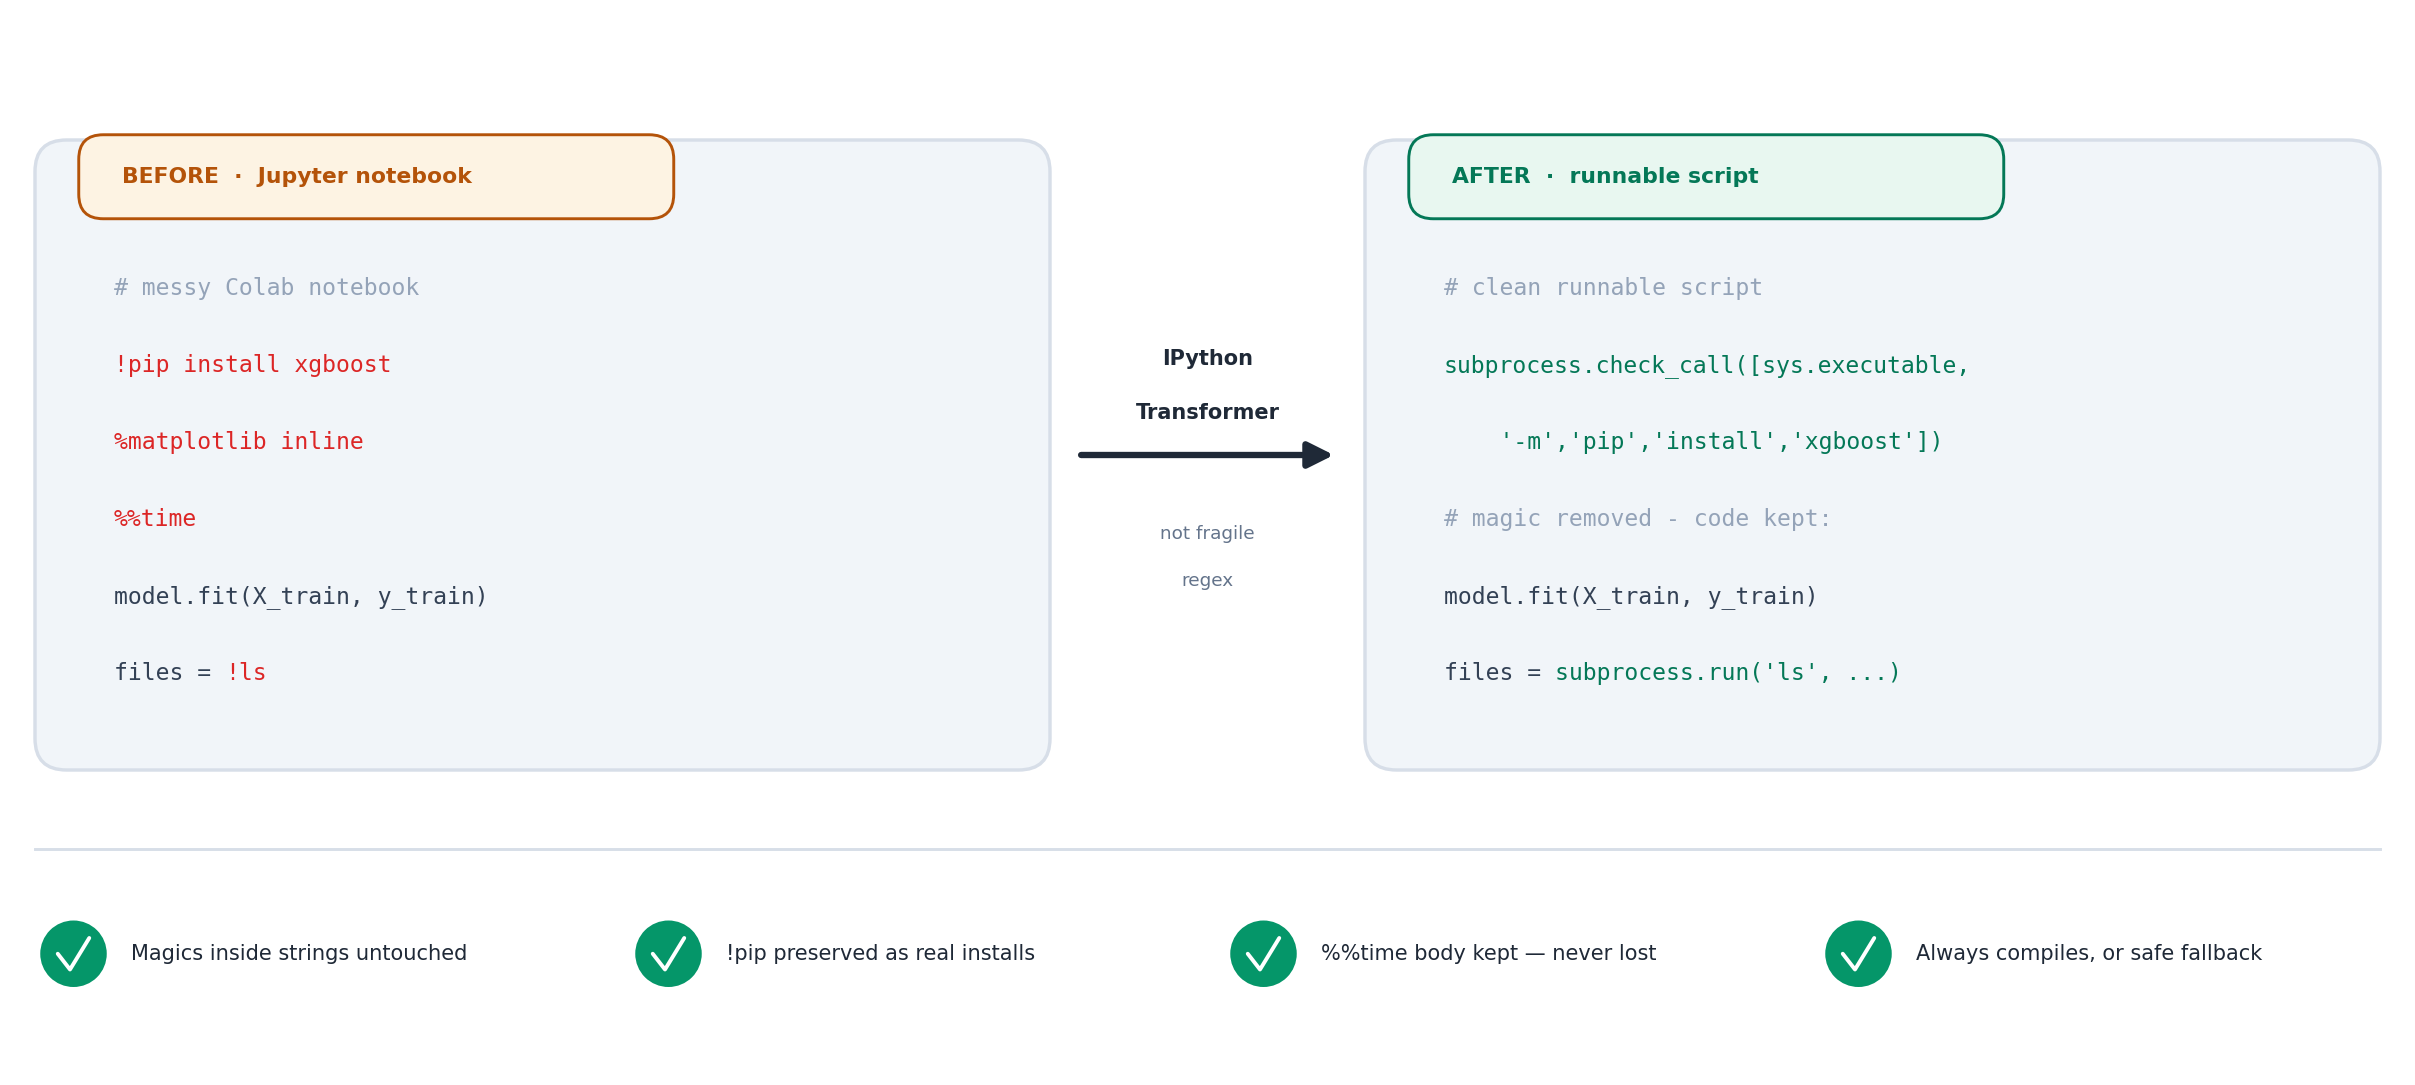
\includegraphics[width=\textwidth,keepaspectratio]{notebook_convert}
  \caption{Notebook-to-script conversion: before and after}
  \label{fig:notebook-convert}
\end{figure}

\subsection{The Training Run}
A training run executes inside an isolated pod, following the training path
designed in Section~\ref{sec:pipeline-org}: download code and dataset, install
missing dependencies (with version pins for known conflicts), and run the
entry script under a generated runner that enables automatic tracking first.
The runner also neutralizes blocking calls (\texttt{plt.show()},
\texttt{input()}) and shims runtime-only modules such as \texttt{google.colab},
so notebooks exported from cloud environments run unchanged. While the run
executes, the backend streams the pod's logs to the browser in real time
(Figure~\ref{fig:screen_logs}).

\bigshot{screen_logs}{The live log terminal}{The training pod's output streams
to the browser as the run executes, so the user follows dependency
installation, notebook conversion, and training in real time.}

\subsection{Experiments Intelligence}
Captured runs are made comparable: the experiments view groups runs by model
family, ranks them on \emph{evaluation} metrics only (never training scores),
flags the champion model, and registers any run as a model version in one
click (Figures~\ref{fig:expintel} and~\ref{fig:screen_experiments}).

\begin{figure}[H]\centering
  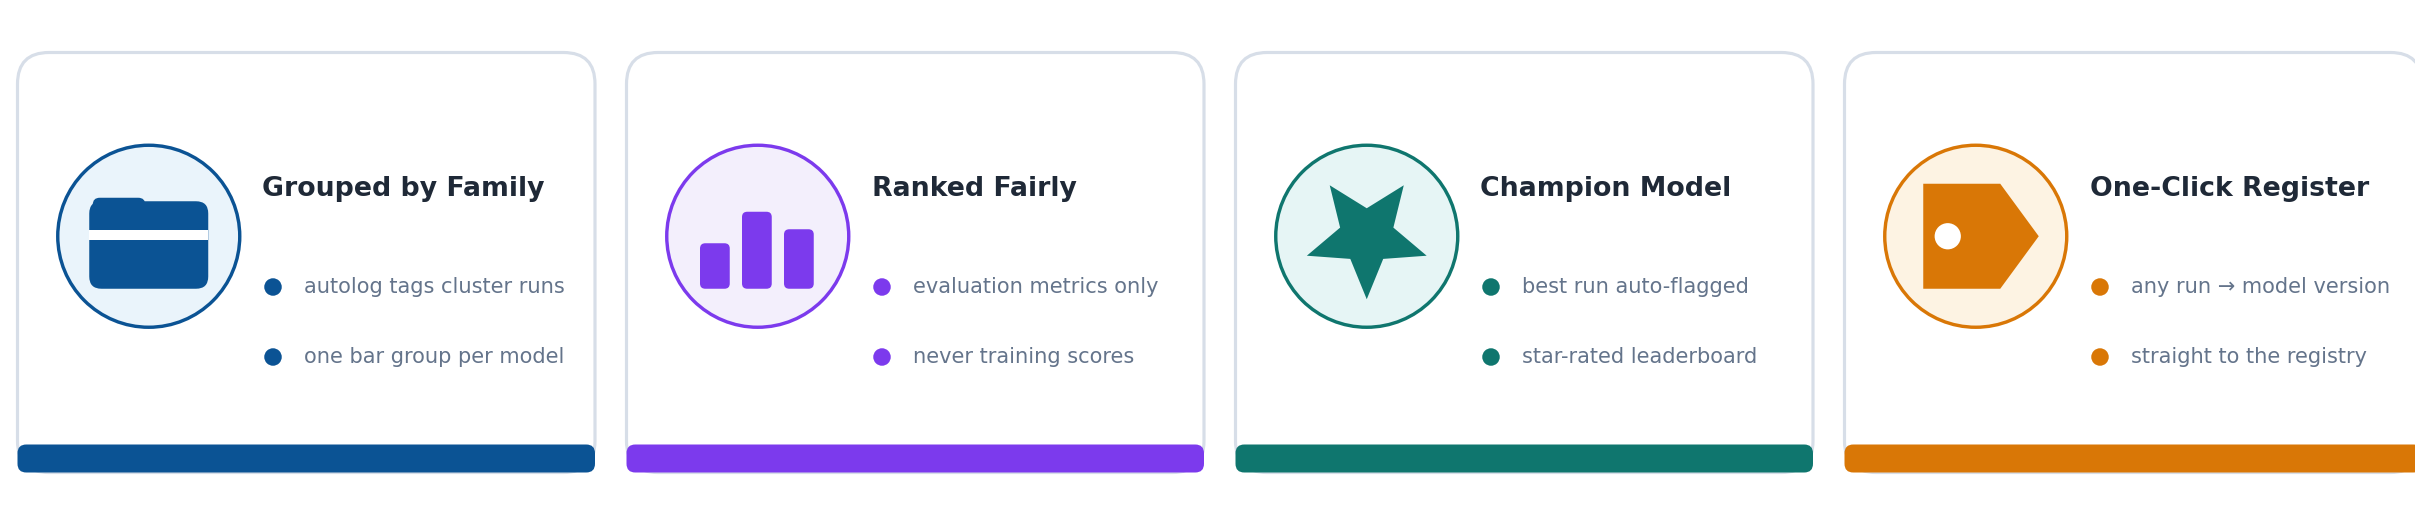
\includegraphics[width=\textwidth,keepaspectratio]{expintel_features}
  \caption{Experiments intelligence: grouping, fair ranking, champion, one-click register}
  \label{fig:expintel}
\end{figure}

\bigshot{screen_experiments}{The experiments view}{Runs are grouped by model
family with their captured metrics, the champion run is highlighted, and any
run can be registered as a model version in one click.}

\subsection{Run Details and Artifact Browser}
\label{sec:artifact-browser}
Each run opens into a detail view: a status header, headline \textbf{metric
cards}, and a searchable parameter list. Its second half is an
\textbf{artifact browser}: the backend lists the run's files directly through
the \gls{s3} \gls{api} and streams any file with its correct content type, so
evaluation plots render inline, folders are navigable, and every file is
downloadable. Both endpoints resolve the run back to a project owned by the
caller and answer \texttt{404} otherwise, so artifacts are never leaked across
users.

\subsection{Sprint Review}
The review demonstrated the full training loop on real notebooks taken from
Colab, not simplified examples. The retrospective identified dependency
conflicts inside training pods as the most frequent failure cause, which
motivated the automatic missing-dependency installation and, later, the
pre-flight code analyzer of Sprint~4.

% ===========================================================================
\section{Sprint 3 --- Registry and Deployment}
\label{sec:sprint3}
The third sprint turns tracked runs into deployable assets: a registry with
lifecycle stages, one-click deployment, and an in-interface prediction tester
(Figure~\ref{fig:sprint3-strip}).

\begin{figure}[H]\centering
  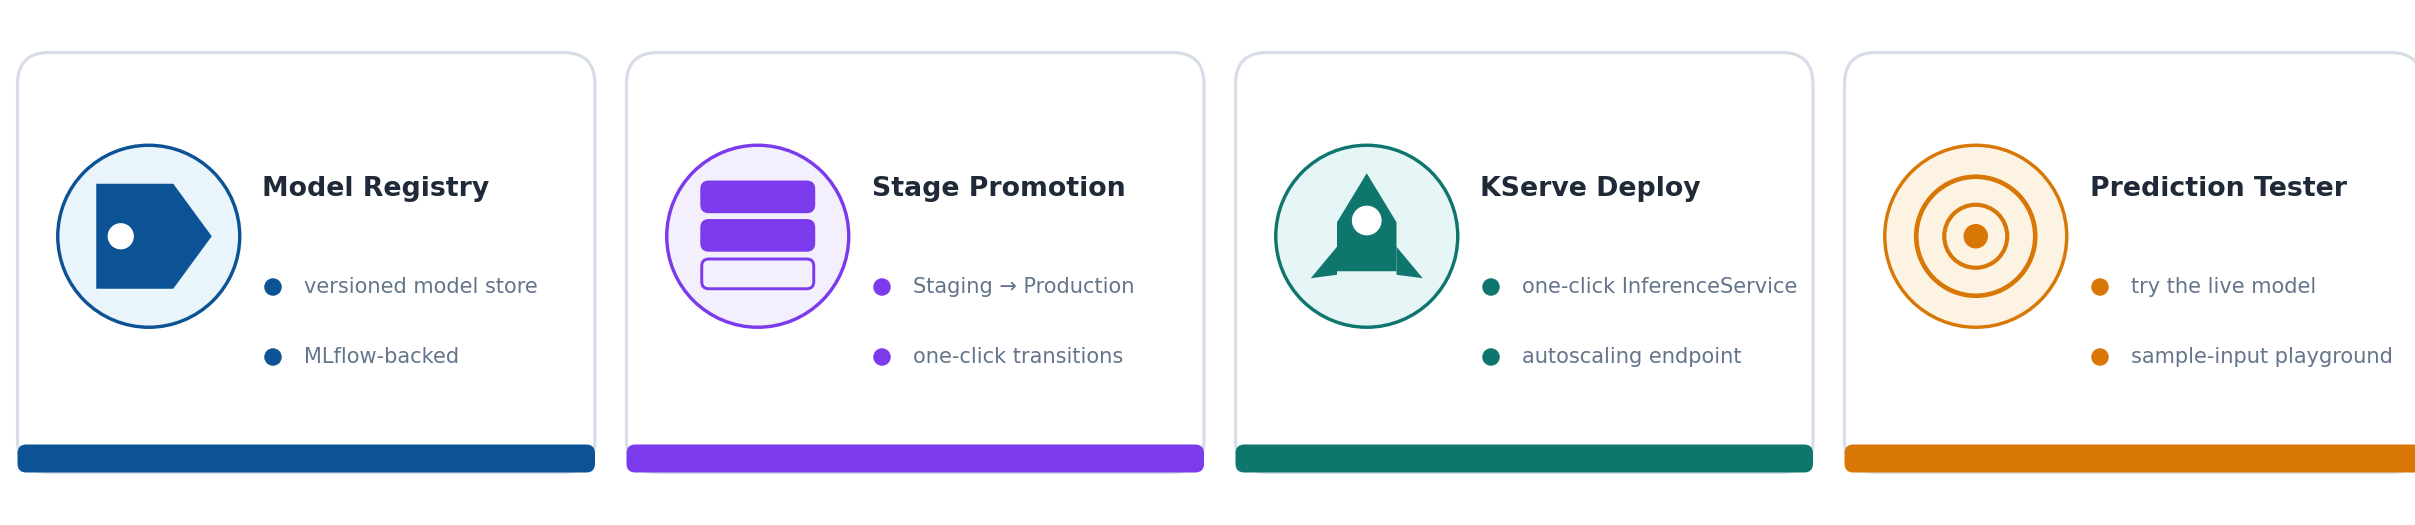
\includegraphics[width=\textwidth,keepaspectratio]{sprint3_features}
  \caption{Sprint 3 at a glance: registry, promotion, KServe deployment, tester}
  \label{fig:sprint3-strip}
\end{figure}

\begin{table}[H]\centering
\renewcommand{\arraystretch}{1.15}
\caption{Sprint~3 backlog}\label{tab:backlog-s3}
\small
\begin{tabularx}{\textwidth}{|c|X|c|}
\hline
\rowcolor{primary!15}
\textbf{\#} & \textbf{Task} & \textbf{Pts}\\
\hline
8  & Register model versions from successful runs & 2\\ \hline
8  & Build the model registry interface & 3\\ \hline
9  & Promote models across Staging/Production/Archived & 3\\ \hline
10 & Deploy a model as an InferenceService on the cluster & 5\\ \hline
10 & Detect the model's framework and serve XGBoost natively & 3\\ \hline
10 & Track deployment status and endpoint & 3\\ \hline
11 & Build the in-UI prediction tester & 5\\ \hline
11 & Surface readable model-server errors to the caller & 2\\ \hline
\end{tabularx}
\end{table}

\subsection{Registry and Promotion}
Successful runs can be registered as named, versioned models. Each version
carries a lifecycle stage (Staging, Production, Archived) that the user
changes from the interface; the tracking server remains the source of truth,
mirrored in the platform's database (Figure~\ref{fig:screen_registry}).

\bigshot{screen_registry}{The model registry}{Each registered version shows its
lifecycle-stage badge (Staging / Production / Archived) and can be promoted or
deployed directly from this view.}

\subsection{One-Click Deployment}
Deploying a model reduces to creating one declarative \texttt{InferenceService}
resource, following the serving path of Section~\ref{sec:pipeline-org}; the
operator reconciles it into a running model server. The backend then polls the
resource's status conditions and updates the deployment record until the
service is \texttt{READY}, so the interface always reflects the real cluster
state (Figure~\ref{fig:screen_deploy}).

\bigshot{screen_deploy}{The deployment panel}{The deployment progresses through
its status conditions to \texttt{READY}, and the live prediction endpoint of
the served model is displayed.}

\subsection{Multi-Framework Serving}
\label{sec:multi-framework}
The serving operator provides one model server per framework, and serving an
XGBoost model through the scikit-learn server fails at startup. The backend
therefore \textbf{detects the framework} at deployment time by listing the
file names in the model's artifact folder: a booster file
(\texttt{model.bst} / \texttt{.json} / \texttt{.ubj} / \texttt{.xgb}) marks an
XGBoost model, anything else defaults to scikit-learn. One incompatibility
remains: MLflow saves XGBoost boosters as \texttt{model.xgb}, a name the
XGBoost server refuses. In that case the backend \emph{materializes} a servable
copy (\texttt{model.xgb} $\rightarrow$ \texttt{model.bst}) in the object store
before creating the service. The user never sees any of this: they click
``Deploy'' and the right runtime serves the right file.

\subsection{Prediction and Error Handling}
\label{sec:prediction-errors}
The backend forwards prediction requests to the model server through the
cluster's \gls{api}, so no model needs a public address; the interface offers
a tester with sample inputs (Figure~\ref{fig:screen_predict}). Failures are
normalized into a dedicated \texttt{PredictionError} with a \emph{readable}
message: when the model server rejects an input, its own error text is returned
with \texttt{502}; when it does not answer in time, the request fails fast with
\texttt{504}. Forwarded predictions run in a worker thread, so a slow model
server never blocks the asynchronous event loop.

\bigshot{screen_predict}{The prediction tester}{The user submits sample inputs
to the deployed model and the returned prediction is displayed, with a readable
error message when an input is malformed.}

\subsection{Sprint Review}
The review showed a model going from a tracked run to a live, tested service
in a few clicks. The retrospective surfaced the framework mismatch between
MLflow's artifacts and the serving runtimes; the automatic framework detection
and booster materialization presented above were the direct outcome.

% ===========================================================================
\section{Sprint 4 --- Observability, Public API, and Administration}
\label{sec:sprint4}
The final sprint makes the platform observable, opens deployed models to the
outside world, and adds administration and diagnostics
(Figure~\ref{fig:sprint4-strip}).

\begin{figure}[H]\centering
  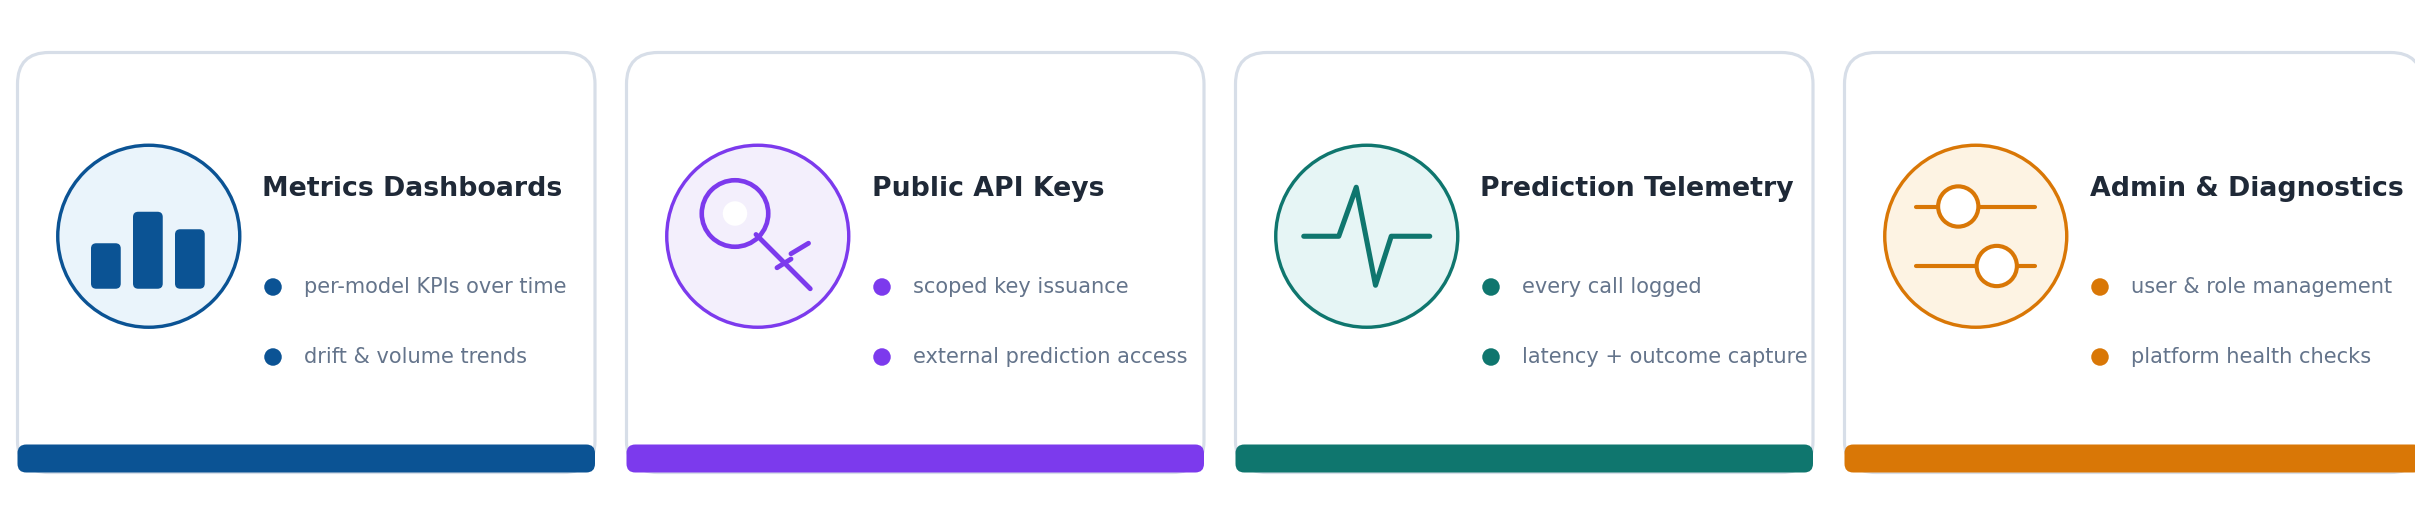
\includegraphics[width=\textwidth,keepaspectratio]{sprint4_features}
  \caption{Sprint 4 at a glance: dashboards, telemetry, API keys, administration}
  \label{fig:sprint4-strip}
\end{figure}

\begin{table}[H]\centering
\renewcommand{\arraystretch}{1.15}
\caption{Sprint~4 backlog}\label{tab:backlog-s4}
\small
\begin{tabularx}{\textwidth}{|c|X|c|}
\hline
\rowcolor{primary!15}
\textbf{\#} & \textbf{Task} & \textbf{Pts}\\
\hline
12 & Collect cluster and per-pod resource metrics & 3\\ \hline
12 & Build the monitoring dashboard & 2\\ \hline
12 & Record per-prediction telemetry and aggregate serving KPIs & 3\\ \hline
13 & Generate and store per-deployment API keys (hashed) & 3\\ \hline
13 & Expose a public, key-authenticated prediction endpoint & 2\\ \hline
14 & Capture and surface user-script errors for failed runs & 3\\ \hline
14 & Add a static pre-flight code analyzer with warnings & 2\\ \hline
15 & Add the administrator role and administration area & 5\\ \hline
\end{tabularx}
\end{table}

\subsection{Cluster Observability}
The backend queries the cluster's metrics service~\cite{metrics_server} for
per-pod \gls{cpu} and memory usage and aggregates cluster-wide figures,
surfaced as live gauges and charts on the dashboard
(Figure~\ref{fig:screen_dashboard}).

\bigshot{screen_dashboard}{The metrics dashboard}{Cluster-wide and per-pod
\gls{cpu} and memory usage are shown as live gauges and charts, so the health
of the cluster and of each deployed model is visible at a glance.}

\subsection{Serving Telemetry and KPIs}
\label{sec:serving-telemetry}
Resource metrics say whether a model server is \emph{running}, not how it is
\emph{behaving}. The platform therefore records one \texttt{PredictionLog} row
for every served prediction --- from the tester or the public \gls{api} ---
with latency, \gls{http} outcome, batch size, and origin. Rows are written
best-effort and contain no payloads.

A per-project endpoint aggregates these rows over a selectable window into the
\glspl{kpi} that matter once a model is live: request volume, error rate,
average and 95\textsuperscript{th}-percentile latency, and a bucketed timeline
rendered as charts in the Monitoring tab.

\subsection{Public Prediction API with API Keys}
Deployment makes a model reachable from inside the platform; this sprint opens
it to the outside world. The owner creates \textbf{per-deployment \gls{api}
keys}: the key (\texttt{mlops\_<random>}) is shown \textbf{once}, only its
\gls{sha}-256 hash and a display prefix are stored, and a key can be revoked
at any time.

External clients call a dedicated public endpoint, outside the
\gls{jwt}-protected \gls{api}, with the key in the \texttt{Authorization}
header; the backend hashes and looks it up, confirms the deployment is ready,
and forwards the request (Figure~\ref{fig:public-api}). Every public call also
lands in the serving telemetry, so external usage is visible in the same
Monitoring tab. A snippet generator produces ready-to-paste cURL, JavaScript,
and Python examples (Figures~\ref{fig:public-api} and~\ref{fig:screen_apikeys}).

\begin{figure}[H]\centering
  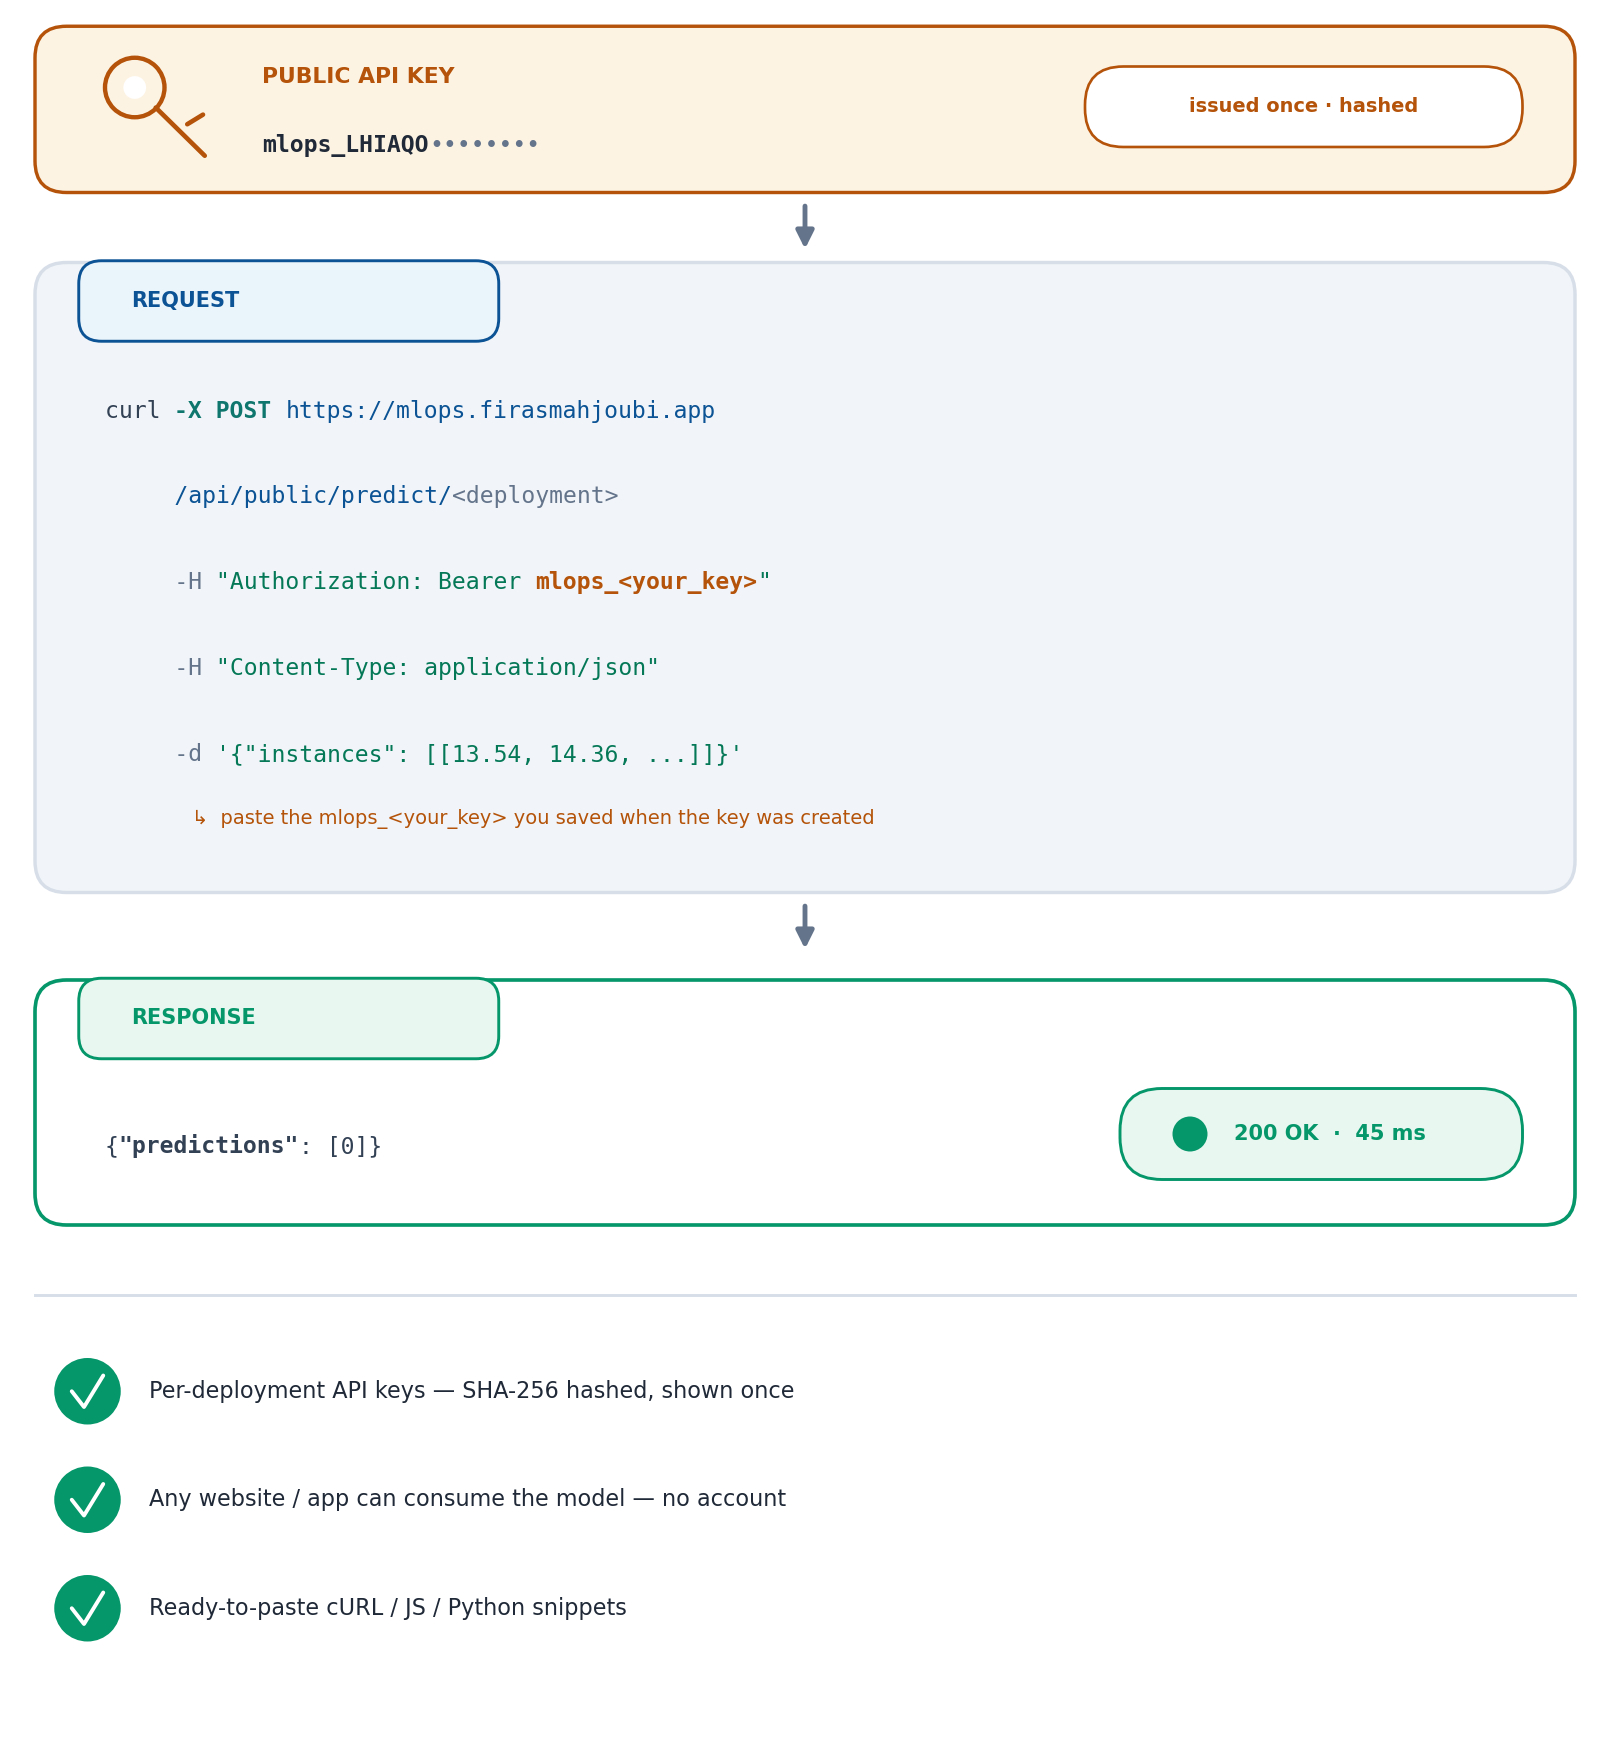
\includegraphics[width=0.9\textwidth,height=0.42\textheight,keepaspectratio]{public_api}
  \caption{Public API flow: key issuance, authenticated request, response}
  \label{fig:public-api}
\end{figure}

\bigshot{screen_apikeys}{The API-keys panel}{Per-deployment keys are created and
revoked here (only their hash is stored), and the code-snippet generator
produces ready-to-paste cURL, JavaScript, and Python calls.}

\subsection{Administration}
A \texttt{role} field distinguishes users from administrators; a backend
dependency guards every administrative endpoint and an Angular guard protects
the routes. The administration area provides user management (activate,
deactivate, promote, demote, purge, delete, with anti-lockout safeguards), a
platform overview, and read-only oversight of all users' resources. Because the
role is read from the database on every request, a demotion takes effect
immediately (Figure~\ref{fig:screen_admin}).

\bigshot{screen_admin}{The administration area}{Every account is listed with its
role and status; an administrator can activate, deactivate, promote, demote,
purge, or delete a user, and oversee all users' resources.}

\subsection{Diagnostics and Robustness}
The platform captures the user-script error of a failed run and stores it
durably, so the interface shows a concise ``why did this fail'' explanation. A
static pre-flight analyzer also inspects uploaded code before launch and warns
about common pitfalls: missing training calls, hard-coded local paths,
notebook-only constructs (Figure~\ref{fig:screen_diagnostics}).

\bigshot{screen_diagnostics}{The failure-explanation panel}{The captured
user-script error is surfaced on the failed run, telling the user \emph{why} it
failed without digging through raw job logs.}

\subsection{Sprint Review}
The final review demonstrated an external client calling a deployed model with
an \gls{api} key and the resulting traffic appearing live in the Monitoring
tab. With administration and diagnostics accepted, the product backlog of
Chapter~\ref{chap:context} was fully delivered.

% ===========================================================================
\section{Continuous Deployment and Environments}
\label{sec:cicd}
The platform itself is delivered like software. Every push to the main branch
triggers a GitHub Actions workflow that builds the backend and frontend
images with registry-backed layer caching, pushes them to \gls{acr}, and
upgrades the Helm release on the \gls{aks} cluster. A concurrency group cancels
any in-progress run when a newer commit arrives, so the cluster always
converges on the latest version of the main branch.

The same Helm chart deploys the full stack to both environments, with only a
values file changing (Table~\ref{tab:environments}).

\begin{table}[H]\centering
\renewcommand{\arraystretch}{1.2}
\caption{Execution environments}\label{tab:environments}
\small
\begin{tabularx}{\textwidth}{|>{\raggedright\arraybackslash}p{3.4cm}|X|X|}
\hline
\rowcolor{primary!15}
\textbf{Aspect} & \textbf{Development (KinD)} & \textbf{Production (AKS)}\\
\hline
Cluster & Kubernetes-in-Docker, local & Azure Kubernetes Service, managed\\ \hline
Purpose & Development and tests & Live, public platform\\ \hline
Images & Loaded locally & Pulled from \gls{acr} by CI/CD\\ \hline
Public access & None (localhost) & Cloudflare Tunnel + managed \gls{tls}\\ \hline
Manifests & \multicolumn{2}{c|}{Same Helm chart, different values file}\\ \hline
\end{tabularx}
\end{table}

% ---------------------------------------------------------------------------
\section{Conclusion}
Four sprints turned the design into a complete platform: identity and
projects, a training-and-tracking engine with notebook conversion, a registry
with one-click multi-framework deployment, and observability with a public
\gls{api} and administration --- all continuously delivered to a production
cluster. The next chapter validates the result, scenario by scenario and on a
real use case.

%==============================================================================
%  CHAPTER 5 — VALIDATION AND RESULTS
%==============================================================================
\chapter{Validation and Results}
\label{chap:validation}

\section{Introduction}
This chapter validates the platform in two complementary ways. First, a
functional validation: every capability delivered by the sprints was exercised
against acceptance scenarios. Second, an end-to-end validation on a
\emph{real} use case: a telecom churn model, trained, tracked, registered,
deployed, and consumed entirely through the platform.

% ---------------------------------------------------------------------------
\section{Functional Validation}
\label{sec:functional-validation}
Each increment was validated manually against its acceptance scenarios before
its sprint closed. Tables~\ref{tab:tests-s1}--\ref{tab:tests-s4} consolidate the
main scenarios, one table per sprint.

\begin{table}[H]\centering
\renewcommand{\arraystretch}{1.15}
\caption{Sprint 1 test scenarios --- Authentication and projects}\label{tab:tests-s1}
\small
\begin{tabularx}{\textwidth}{|X|X|c|}
\hline
\rowcolor{primary!15}
\textbf{Scenario} & \textbf{Expected result} & \textbf{Status}\\
\hline
Sign up, then sign in & Tokens issued; redirect to dashboard & OK\\ \hline
Sign in with wrong password & \texttt{401}, no token issued & OK\\ \hline
Access token expiry & Session silently renewed via refresh token & OK\\ \hline
Create a project & Stored and bound to a new tracking experiment & OK\\ \hline
Open another user's project & \texttt{404}, resource invisible & OK\\ \hline
\end{tabularx}
\end{table}

\begin{table}[H]\centering
\renewcommand{\arraystretch}{1.15}
\caption{Sprint 2 test scenarios --- Training and tracking}\label{tab:tests-s2}
\small
\begin{tabularx}{\textwidth}{|X|X|c|}
\hline
\rowcolor{primary!15}
\textbf{Scenario} & \textbf{Expected result} & \textbf{Status}\\
\hline
Upload a \texttt{.zip} without an entry script & Entry script auto-detected by priority order & OK\\ \hline
Run a scikit-learn script & Metrics, parameters, and model captured automatically & OK\\ \hline
Run a real-world Colab notebook & Converted at upload, shims applied, run succeeds & OK\\ \hline
Run a script with a missing dependency & Dependency installed in the pod before execution & OK\\ \hline
Run a failing script & Run marked failed; readable reason shown on the run & OK\\ \hline
Watch logs during a run & Log lines stream live to the browser & OK\\ \hline
Open a run's artifacts & Folders navigable; images preview; files download & OK\\ \hline
Request another user's artifacts & \texttt{404}, the run is not revealed & OK\\ \hline
\end{tabularx}
\end{table}

\begin{table}[H]\centering
\renewcommand{\arraystretch}{1.15}
\caption{Sprint 3 test scenarios --- Registry and deployment}\label{tab:tests-s3}
\small
\begin{tabularx}{\textwidth}{|X|X|c|}
\hline
\rowcolor{primary!15}
\textbf{Scenario} & \textbf{Expected result} & \textbf{Status}\\
\hline
Register a run, promote to Production & Version and stage updated in registry and interface & OK\\ \hline
Deploy a registered model & InferenceService created; status reaches READY & OK\\ \hline
Deploy an XGBoost model & Framework detected; booster materialized; served natively & OK\\ \hline
Predict with the wrong feature count & Readable \texttt{502} carrying the model server's message & OK\\ \hline
Delete a deployment & Cluster resources removed; record cleaned up & OK\\ \hline
\end{tabularx}
\end{table}

\begin{table}[H]\centering
\renewcommand{\arraystretch}{1.15}
\caption{Sprint 4 test scenarios --- Public API, monitoring, administration}\label{tab:tests-s4}
\small
\begin{tabularx}{\textwidth}{|X|X|c|}
\hline
\rowcolor{primary!15}
\textbf{Scenario} & \textbf{Expected result} & \textbf{Status}\\
\hline
Call the public endpoint with a valid key & Prediction returned without a platform account & OK\\ \hline
Call with a revoked key & \texttt{401} & OK\\ \hline
Send predictions, open the Monitoring tab & Volume, error rate, latency, per-origin and per-deployment breakdown reflect the calls & OK\\ \hline
Call an admin endpoint as a normal user & \texttt{403} & OK\\ \hline
Administrator attempts self-demotion & Refused with an explanatory error & OK\\ \hline
\end{tabularx}
\end{table}

% ---------------------------------------------------------------------------
\section{End-to-End Case Study: Telecom Churn}
\label{sec:case-study}

\subsection{Scenario}
The platform was validated with a real churn-prediction use case built on
operational data from a regional telecom operator: a file of terminated
customers and a file of network incidents, joined and transformed into
customer-level features by a Jupyter notebook. The complete journey runs
through the platform only (Figure~\ref{fig:casestudy-journey}): the notebook
and its two Excel files are uploaded as one zip; the notebook is
\textbf{automatically converted} to a script (Section~\ref{sec:sprint2});
the run executes on the cluster with autolog capturing every metric; the best
model is registered, promoted, deployed, and finally called from outside
through the public \gls{api}.

\begin{figure}[H]\centering
  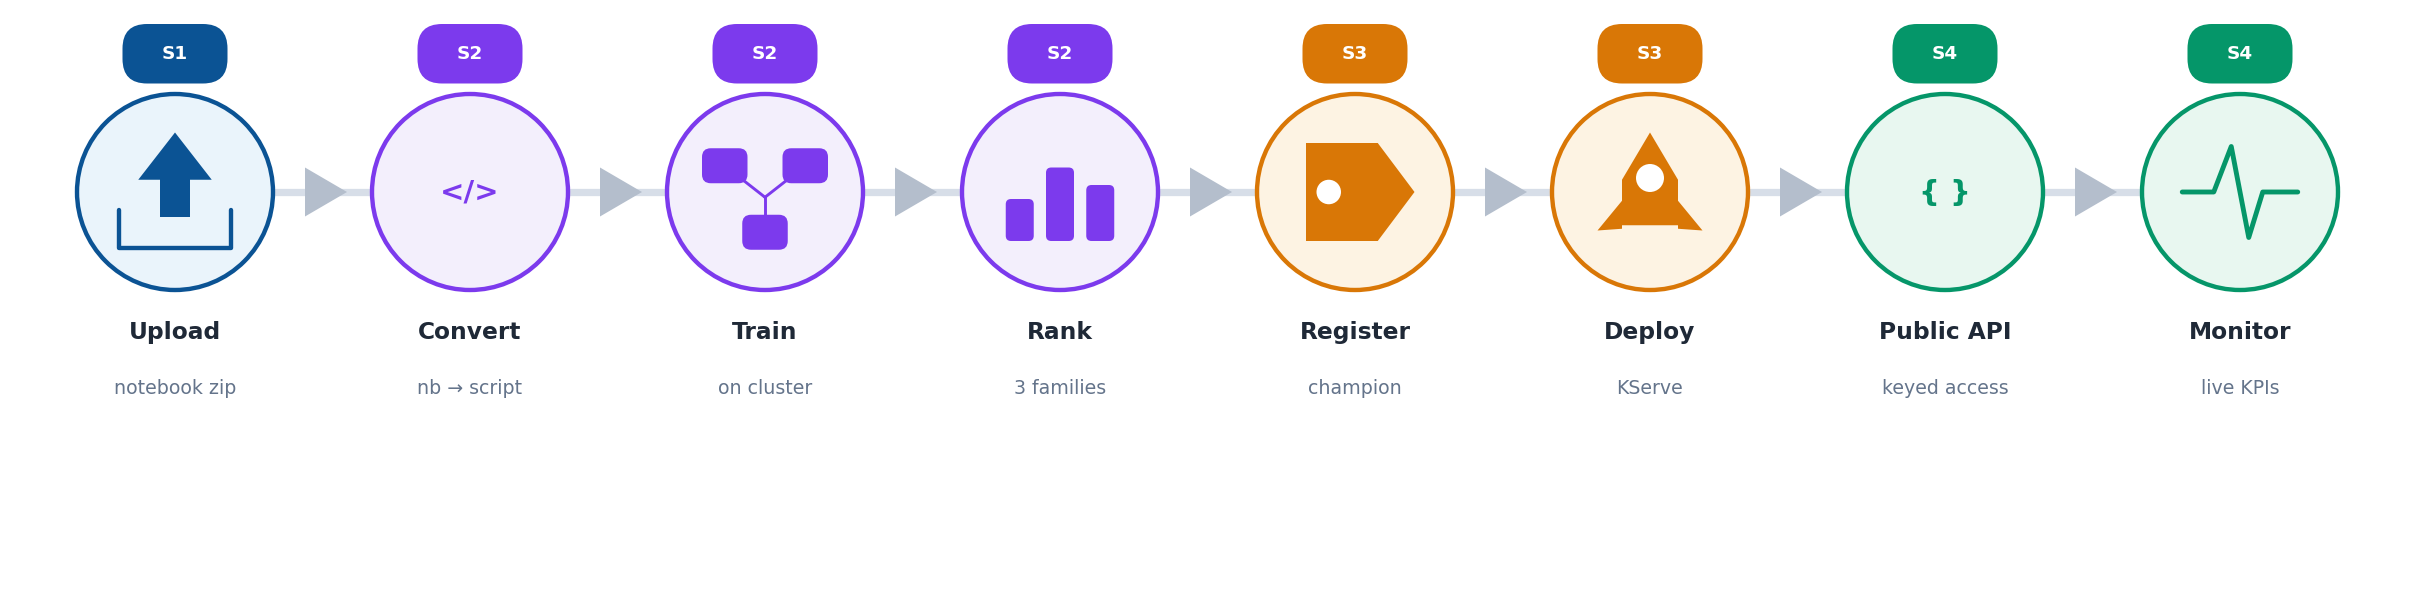
\includegraphics[width=\textwidth,keepaspectratio]{casestudy_journey}
  \caption{Case-study journey: one dataset, the full lifecycle on the platform}
  \label{fig:casestudy-journey}
\end{figure}

\subsection{Evaluation Metrics}
Churn data is imbalanced: most clients stay, few leave. Three complementary
metrics are therefore used. \textbf{Accuracy} measures overall correctness but
can be inflated by the majority class. The \textbf{F1-score} focuses on the
churn class only, combining precision (are the raised alerts correct?) and
recall (how many real churners are caught?), so it cannot be gamed by
predicting ``no churn'' everywhere. The \textbf{\gls{roc}-\gls{auc}} evaluates
the model's \emph{ranking}: the probability that a random churner receives a
higher risk score than a random non-churner, independently of any decision
threshold --- the right measure when the business goal is ``call the most
at-risk clients first''.

\subsection{Model and Results}
The model is an XGBoost classifier trained on an 80/20 split, with SMOTE
applied to the training part to compensate for class imbalance.
Table~\ref{tab:churn-metrics} reports the evaluation results captured by the
platform, and Table~\ref{tab:churn-cm} the confusion matrix on the test set.

\begin{table}[H]\centering
\renewcommand{\arraystretch}{1.2}
\caption{Churn model: evaluation metrics (test set)}\label{tab:churn-metrics}
\small
\begin{tabularx}{\textwidth}{|X|c|X|}
\hline
\rowcolor{primary!15}
\textbf{Metric} & \textbf{Value} & \textbf{Reading}\\
\hline
Accuracy & 0.881 & Overall correctness on all clients\\ \hline
F1-score (churn class) & 0.773 & Balance of precision and recall on churners\\ \hline
ROC-AUC & 0.911 & Excellent ranking of clients by churn risk\\ \hline
ROC-AUC (5-fold CV) & $\approx$ 0.91 & Stable across folds --- no overfitting to one split\\ \hline
\end{tabularx}
\end{table}

\begin{table}[H]\centering
\renewcommand{\arraystretch}{1.2}
\caption{Churn model: confusion matrix (test set)}\label{tab:churn-cm}
\small
\begin{tabular}{|l|c|c|}
\hline
\rowcolor{primary!15}
 & \textbf{Predicted: active} & \textbf{Predicted: churn}\\
\hline
\textbf{Real: active} & 669 & 35\\ \hline
\textbf{Real: churn}  & 87  & 201\\ \hline
\end{tabular}
\end{table}

The business reading confirms the ranking quality measured by the
\gls{roc}-\gls{auc}: when clients are sorted by predicted risk, the low-risk
segment contains about 5\% real churners, the medium segment about 27\%, and
the high-risk segment about \textbf{96\%} --- exactly the list a retention
team should call first (Figure~\ref{fig:casestudy-proof}).

\begin{figure}[H]\centering
  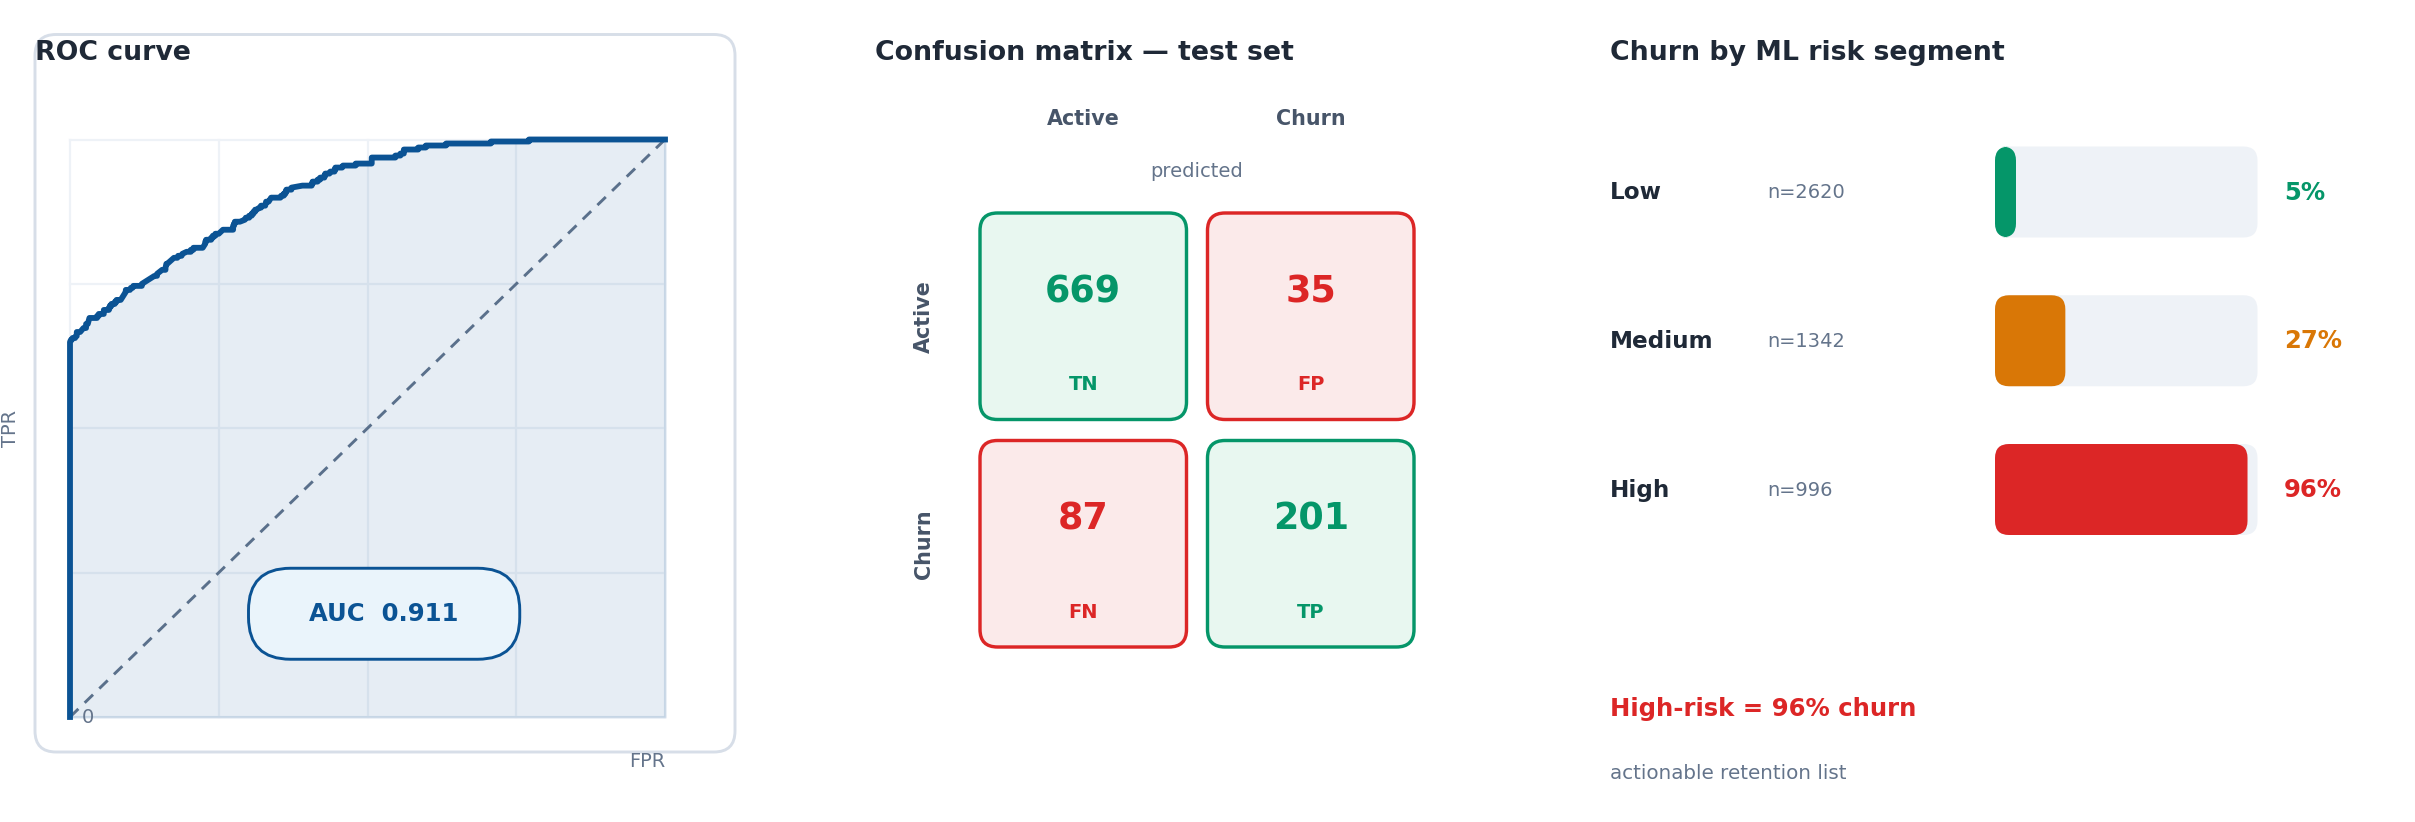
\includegraphics[width=\textwidth,keepaspectratio]{casestudy_proof}
  \caption{Case-study results: real metrics and risk segments}
  \label{fig:casestudy-proof}
\end{figure}

\bigshot{screen_churn_deploy}{The churn model, registered and deployed}{The
champion run for this case study, registered from the leaderboard and deployed
as a live \texttt{InferenceService}: the platform's own registry and
deployment record for the exact model behind the metrics above, status
\texttt{READY}.}

\subsection{Consuming the Model from Outside}
To close the loop, the deployed churn model was called from an external
\gls{http} client using a per-deployment \gls{api} key, exactly as a
third-party retention application would (Listing~\ref{lst:churn-call}). The
15 values are the model's actual training features, in order ---
\texttt{nb\_reclamations}, \texttt{delai\_moy\_resolution},
\texttt{delai\_max\_resolution}, \texttt{delai\_min\_resolution},
\texttt{delai\_std\_resolution}, \texttt{nb\_incidents\_longs},
\texttt{nb\_non\_resolus}, \texttt{nb\_categories\_distinctes},
\texttt{a\_eu\_reclamation}, \texttt{ratio\_non\_resolu},
\texttt{ratio\_incidents\_longs}, \texttt{score\_risque}, \texttt{debit\_num},
\texttt{fsi\_encoded}, \texttt{cat\_encoded} --- and the response below is a
real capture, not an illustration. The call and its latency then appear in the
project's Monitoring tab.

\begin{lstlisting}[language=bash,caption={External prediction call against the deployed churn model (real request/response capture).},label={lst:churn-call}]
curl -X POST "https://mlops.firasmahjoubi.app/api/public/predict/<deployment_id>" \
  -H "Authorization: Bearer mlops_<key>" \
  -H "Content-Type: application/json" \
  -d '{"instances": [[5, 8.5, 15, 2, 4.2, 2, 1, 3, 1, 0.2, 0.4, 18.55, 8, 2, 1]]}'

{"predictions":[0.03778325021266937]}   % churn risk of this client: 3.8%
\end{lstlisting}

This exact call initially failed with a \texttt{502} carrying \emph{``training
data did not have the following fields: nb\_reclamations, \ldots''} ---
XGBoost's booster embeds the training \texttt{DataFrame}'s column names,
and the public/tester endpoints send a plain, unnamed array, so the model
server rejected every request for this deployment. The fix strips
\texttt{feature\_names}/\texttt{feature\_types} from the booster before it is
saved as the servable \texttt{model.bst} (Section~\ref{sec:sprint3}), so an
unnamed array matches what the booster now expects. Applied to this
deployment's artifact and the predictor pod restarted, the same call now
returns \texttt{200} with a real prediction, as captured above.

\bigshot{screen_churn_monitoring}{Live traffic from the external call}{The
churn deployment's Monitoring tab immediately after the Postman call above:
the request is counted, its latency measured, and it is attributed to the
public \gls{api} origin --- closing the loop from an outside \gls{http} client
to the platform's own serving telemetry.}

\subsection{What the Case Study Demonstrates}
This single use case exercises every layer built in the four sprints:
\begin{itemize}[leftmargin=1.4em]
  \item the \textbf{notebook conversion} handled a real, messy notebook
        (Excel dependencies, \texttt{!pip install}, French text) without
        manual editing;
  \item \textbf{autolog} captured all parameters, metrics, and evaluation
        artifacts with zero code changes;
  \item the \textbf{leaderboard} exposed the metrics above and flagged the
        champion run;
  \item \textbf{multi-framework serving} detected the XGBoost booster and
        materialized a servable file automatically;
  \item the deployed model answered predictions from the in-platform tester
        and from an external \gls{http} client through a hashed \gls{api}
        key, with every call visible in the \textbf{serving telemetry}.
\end{itemize}

% ---------------------------------------------------------------------------
\section{Conclusion}
The platform passed its functional scenarios across all four sprints, and a
real churn model traveled the full lifecycle --- upload, automatic conversion,
tracked training (\gls{roc}-\gls{auc} 0.911), registration, deployment, public
consumption, monitoring --- without a single line of infrastructure code
written by the data scientist. This is precisely the objective fixed in
Chapter~\ref{chap:context}.

\input{chapters/06_general_conclusion}

%---------------------------------------------------------------- back matter
\cleardoublepage
\phantomsection
\addcontentsline{toc}{chapter}{Bibliography}
\printbibliography[title={Bibliography}]

\appendix
%==============================================================================
%  APPENDICES
%==============================================================================
\chapter{REST API Reference}
\label{app:api}

This annex lists the platform's main \gls{rest} endpoints. All routes below are
prefixed with \texttt{/api/v1} and require a \gls{jwt} access token, except the
authentication routes and the public prediction endpoint, which is mounted under
\texttt{/api/public} and authenticated by \gls{api} key. Administrative routes
additionally require the administrator role.

\begin{table}[H]\centering
\renewcommand{\arraystretch}{1.2}
\caption{REST endpoints: authentication, projects, pipelines, and experiments}
\label{tab:api-ref}
\footnotesize
\begin{tabularx}{\textwidth}{|p{2.1cm}|p{5.6cm}|X|}
\hline
\textbf{Method} & \textbf{Path} & \textbf{Purpose}\\
\hline
\multicolumn{3}{|l|}{\cellcolor{primary!12}\textbf{Authentication}}\\ \hline
POST & \texttt{/auth/signup} & Create an account; returns a token pair\\ \hline
POST & \texttt{/auth/login} & Authenticate; returns a token pair\\ \hline
POST & \texttt{/auth/refresh} & Renew the access token\\ \hline
GET  & \texttt{/auth/me} & Current user profile (including role)\\ \hline
\multicolumn{3}{|l|}{\cellcolor{primary!12}\textbf{Projects and uploads}}\\ \hline
GET / POST & \texttt{/projects} & List own projects / create a project\\ \hline
GET / PUT / DELETE & \texttt{/projects/\{id\}} & Read, update, or delete a project\\ \hline
POST & \texttt{/uploads/upload} & Upload code or dataset to a project\\ \hline
POST & \texttt{/uploads/files/analyze} & Pre-flight static analysis of uploaded code\\ \hline
\multicolumn{3}{|l|}{\cellcolor{primary!12}\textbf{Pipelines and experiments}}\\ \hline
POST & \texttt{/pipelines/trigger-custom} & Run the uploaded code as a pipeline\\ \hline
GET  & \texttt{/pipelines/\{run\_id\}/logs} & Live logs of a run\\ \hline
GET  & \texttt{/pipelines/\{run\_id\}/error} & Captured failure reason of a run\\ \hline
GET  & \texttt{/experiments/project/\{id\}} & Runs of a project with metrics\\ \hline
GET  & \texttt{/experiments/compare} & Compare metrics across runs\\ \hline
\end{tabularx}
\end{table}

\begin{table}[H]\centering
\renewcommand{\arraystretch}{1.2}
\caption{REST endpoints: models, deployments, public API, and administration}
\label{tab:api-ref2}
\footnotesize
\begin{tabularx}{\textwidth}{|p{2.1cm}|p{5.6cm}|X|}
\hline
\textbf{Method} & \textbf{Path} & \textbf{Purpose}\\
\hline
\multicolumn{3}{|l|}{\cellcolor{primary!12}\textbf{Models and deployments}}\\ \hline
GET  & \texttt{/models/\{name\}/versions} & Versions of a registered model\\ \hline
POST & \texttt{/models/\{name\}/versions/\{v\}/ promote} & Change a version's lifecycle stage\\ \hline
POST & \texttt{/deployments} & Deploy a model as an InferenceService\\ \hline
POST & \texttt{/deployments/\{id\}/predict} & Authenticated in-platform prediction\\ \hline
POST / GET & \texttt{/deployments/\{id\}/api-keys} & Create / list public API keys\\ \hline
DELETE & \texttt{/deployments/\{id\}/api-keys/ \{kid\}} & Revoke a key\\ \hline
\multicolumn{3}{|l|}{\cellcolor{primary!12}\textbf{Public (API-key authenticated)}}\\ \hline
POST & \texttt{/api/public/predict/\{id\}} & Prediction for external clients\\ \hline
\multicolumn{3}{|l|}{\cellcolor{primary!12}\textbf{Monitoring and administration}}\\ \hline
GET  & \texttt{/cluster/metrics} & Cluster and per-pod resource metrics\\ \hline
GET  & \texttt{/admin/users} & List all accounts (admin)\\ \hline
PATCH / DELETE & \texttt{/admin/users/\{id\}} & Update role/status or delete (admin)\\ \hline
POST & \texttt{/admin/users/\{id\}/purge} & Purge a user's resources (admin)\\ \hline
GET  & \texttt{/admin/overview} & Platform-wide statistics (admin)\\ \hline
\end{tabularx}
\end{table}

%==============================================================================
\chapter{Continuous Deployment Pipeline}
\label{app:cicd}

Every push to the main branch triggers a GitHub Actions workflow that builds and
deploys the platform. The workflow authenticates to Azure, builds the backend and
frontend container images with registry-backed layer caching, pushes them to
\gls{acr}, and upgrades the Helm release on the \gls{aks} cluster. A concurrency
group cancels any in-progress run when a newer commit arrives, so the cluster
always converges on the latest version of the main branch.

\begin{lstlisting}[caption={Excerpt of the GitHub Actions deployment workflow.},label={lst:cicd}]
name: Build and deploy to AKS
on:
  push:
    branches: [main]
  workflow_dispatch:

env:
  ACR_LOGIN_SERVER: acrmlopspfedemo.azurecr.io
  AKS_CLUSTER: aks-mlops-pfe
  HELM_RELEASE: mlops

jobs:
  deploy:
    runs-on: ubuntu-latest
    concurrency:
      group: deploy-main
      cancel-in-progress: true
    steps:
      - uses: actions/checkout@v4
      - uses: docker/setup-buildx-action@v3
      # ... az login, ACR auth ...
      # build + push backend and frontend images (cache-from/to ACR)
      # helm upgrade --install with the new image tags
\end{lstlisting}

The deployment itself is described by a Helm chart that templates every
Kubernetes resource of the platform (backend, frontend, database, object store,
tracking server, tunnel agent), so the same chart deploys the full stack to the
local development cluster and to \gls{aks} with only a values file changing.


%==============================================================================
%  BACK COVER  (last page: résumé + abstract + keywords, no page number)
%==============================================================================
\clearpage
\thispagestyle{empty}
\vspace*{0.5cm}

\begin{center}
{\large\bfseries\color{primary} Design and Implementation of an End-to-End MLOps
Platform}\\[0.2cm]
{\normalsize Firas Mahjoubi}
\end{center}

\vspace{0.8cm}
\noindent\rule{\textwidth}{0.8pt}
\begin{otherlanguage}{french}
\subsection*{R\'esum\'e}
Ce projet de fin d'\'etudes, r\'ealis\'e au sein d'INSOMEA, porte sur la conception
et la r\'ealisation d'une plateforme MLOps compl\`ete et auto-h\'eberg\'ee qui
automatise le cycle de vie de l'apprentissage automatique : gestion de projets,
ex\'ecution des entra\^inements sur Kubernetes avec suivi automatique des
exp\'eriences, registre et promotion des mod\`eles, d\'eploiement comme services
de pr\'ediction, exposition s\'ecuris\'ee par cl\'es API publiques, supervision et
administration. Le syst\`eme repose sur FastAPI, Angular, Kubeflow Pipelines,
MLflow, KServe, MinIO et PostgreSQL, et est d\'eploy\'e en continu sur Azure
Kubernetes Service. Le travail a \'et\'e conduit avec la m\'ethode Scrum en quatre
sprints.

\noindent\textbf{Mots cl\'es :} MLOps, Kubernetes, apprentissage automatique,
d\'eploiement de mod\`eles, MLflow, KServe, Scrum.
\end{otherlanguage}

\noindent\rule{\textwidth}{0.8pt}
\subsection*{Abstract}
This end-of-studies project, carried out within INSOMEA, covers the design and
implementation of a complete, self-hosted MLOps platform that automates the
machine-learning lifecycle: project management, training execution on Kubernetes
with automatic experiment tracking, model registry and promotion, deployment as
live prediction services, secure exposure through public API keys, monitoring,
and administration. The system is built with FastAPI, Angular, Kubeflow
Pipelines, MLflow, KServe, MinIO, and PostgreSQL, and is continuously deployed to
Azure Kubernetes Service. The work was managed with the Scrum method over four
sprints.

\noindent\textbf{Keywords:} MLOps, Kubernetes, machine learning, model
deployment, MLflow, KServe, Scrum.

\noindent\rule{\textwidth}{0.8pt}
\begin{center}
{\small Host organization: \textbf{INSOMEA} \quad|\quad
ESPRIT, Software Engineering \quad|\quad Academic year 2025--2026}
\end{center}


\end{document}
